% Gelfand seminar notes, 1966-67: source pages P000140-P000207.
% Russian diplomatic transcription (AI-made, checked against the scans), cut page by page from the cumulative working reader A4-reader-chapters01-20-first1000-separated-diplomatic-r2.
% \SourcePage{GELFAND-Pnnnnnn}{label} starts a scanned page; the second argument is the number written
% on the page, if any. Editorial notes give the page, a label and the transcriber's remark; \Unclear
% marks a doubtful reading.
\SourcePage{GELFAND-P000140}{5}
\underline{Семинар} \underline{Гельфанда.}\quad $5/\overline{\underline{\mathrm{IX}}}$

1. Систематически будет \uwave{статфизика.} (Минлос)

2. Состояние \uwave{псевдодифференциальных} операторов. (Вишик и Агранович)

3. \uwave{Алгебраические группы} (Кириллов)

\begin{flushright}
\begin{tikzpicture}[x=1cm,y=1cm,baseline=(p.base)]
\node (p) at (.35,.35) {$5$};
\draw[line width=.6pt] (0,.8) -- (0,0) -- (.9,0);
\end{tikzpicture}
\end{flushright}

\begin{GelfandAdjacentEvidence}{GELFAND-P000140}{1}
\uwave{Ценная информация:} лекции Atiyah по $K$-функтору не требуют предв. знаний, кроме опред. топологич. пр-ва и $n$-мерного векторного пр-ва
(По степени про-зрачности\,[?] не сравнимо даже с Милнором)
\Unclear{GELFAND-P000140}{Atiyah-prerequisites}{В слове «про-зрачности» короткая черта после «про»: дефис / соединительный штрих письма; чтение слова сохранено с этой оговоркой.}
\end{GelfandAdjacentEvidence}

4. \uwave{Деформации} всякого рода. (условное название: нелинейный анализ), в том числе \dashuline{Kodaira} и \dashuline{Spencer}.

\begin{GelfandAdjacentEvidence}{GELFAND-P000140}{2}
\uuline{Результат Hirzebruch'a.} (Гельфанд)
\begin{gather*}
\left\{\begin{aligned}
z_1^3+z_2^{3k-1\text{[?]}}+z_3^2+z_4^2+z_5^2&=0\\
|z_1|^2+|z_2|^2+|z_3|^{2\text{[?]}}+|z_4|^2\mathbin{+\text{[?]}}|z_5|^2&=\varepsilon
\end{aligned}\right.
\end{gather*}
\hfill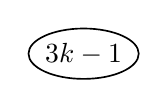
\begin{tikzpicture}[x=1cm,y=1cm,baseline=(e.base)]
\node (e) at (0,0) {$3k-1$};
\draw[line width=.6pt] (0,0) ellipse (.7cm and .32cm);
\end{tikzpicture}\par
\Unclear{GELFAND-P000140}{z2-overwritten-exponent}{Показатель при $z_2$ начинается $3k$; конец густо переписан: $3k-1$ / иной переписанный конец. Справа отдельно обведено овалом $3k-1$. При $z_1$ написан показатель $3$.}
\end{GelfandAdjacentEvidence}


\begin{GelfandAdjacentEvidence}{GELFAND-P000140}{3}
\Unclear{GELFAND-P000140}{modulus-overwrite}{Во второй строке правая черта и показатель при $|z_3|$ густо переписаны; $|z_3|^2$ дано с этой оговоркой. Между $|z_4|^2$ и $|z_5|^2$ знак похож на $+$, но густой.}
\end{GelfandAdjacentEvidence}
\begin{GelfandAdjacentEvidence}{GELFAND-P000140}{4}

10 неизв. и [зачёркнутый неразобранный фрагмент] 3 ур-я
\Unclear{GELFAND-P000140}{cancelled-equation-count}{Зачёркнутый короткий фрагмент после «и»: $7$-подобный знак и дальнейшие густые штрихи; исходное содержание неразборчиво.}
\end{GelfandAdjacentEvidence}

\underline{Милнор:} это гомеоморфно $S^7$

\uwave{Хирцебрух:} при $k=1,2,\ldots,28$ там разные дифф. структуры, а дальше всё повторяется периодически и это все милноровские сферы.

$S^{11}$ есть 992 штуки и они получаются такими уравнениями.



\begin{GelfandAdjacentEvidence}{GELFAND-P000141}{1}
\SourcePage{GELFAND-P000141}{unlabelled}
\uuline{Bass} (Каждан\,[?])\quad \underline{жёсткость арифм. подгрупп.}
\Unclear{GELFAND-P000141}{speaker-name}{Третья буква фамилии между «Ка» и «дан» написана густым соединённым штрихом: «Каждан» / «Каздан».}
\end{GelfandAdjacentEvidence}

\underline{$SL(n,Z)\subset SL(n,R)$ — жёсткая подгруппа,}

\begin{GelfandAdjacentEvidence}{GELFAND-P000141}{2}
[Зачёркнуты короткое начало строки и слово перед «всякая».]
\Unclear{GELFAND-P000141}{cancelled-introduction}{Начальное зачёркнутое обозначение похоже на «II.» / «Те.», следующее густо зачёркнутое слово не читается.}
\end{GelfandAdjacentEvidence}

всякая деформация, (т.е. отобр.)
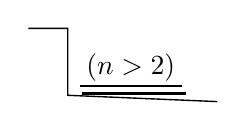
\begin{tikzpicture}[x=1cm,y=1cm,baseline=(d.base)]
\node (d) at (.8,.35) {$(n>2)$};
\draw[line width=.5pt] (-.5,.85) -- (0,.85) -- (0,0) -- (1.9,-.08);
\draw[line width=.5pt] (.15,.12) -- (1.45,.12);
\draw[line width=.9pt] (.18,.025) -- (1.5,.025);
\end{tikzpicture}
\begin{equation*}SL(n,Z)\times[0,1]\longrightarrow SL(n,R)\end{equation*}

к-рое непрерывно и $\forall t\in[0,1]$ гомоморфизм, при $t=0$ это вложение) тривиальна, т.е. она есть внутр. автоморфизм отн. $g(t)$ (кривая в группе)
\begin{equation*}\varphi(h\times t)=g(t)h\cdot g(t)^{-1},\qquad h\in SL(n,Z)\end{equation*}

Теорема Вейля док. лишь для случая, когда факторпр-во компактно.

Зад. свод. к задаче о конгруэнцподгр. над конечным полем.
(Если есть два гомоморф., то неизв., можно ли их соединить)

\begin{GelfandAdjacentEvidence}{GELFAND-P000141}{3}
Существ. деформ. — нетрив.
\begin{center}
\begin{tikzpicture}[x=1cm,y=1cm]
\node at (0,0) {$H^1(\Gamma,\mathfrak g)\mathord{:}\mathord{*}\text{[?]}$};
\node at (3.1,0) {(Borel, Bass)};
\node at (.7,-.75) {конечн. число образ.};
\draw[->,line width=.7pt] (-.7,-.5) -- (-.7,-.24);
\end{tikzpicture}
\end{center}
\Unclear{GELFAND-P000141}{cohomology-terminal}{После $H^1(\Gamma,\mathfrak g)$ стоят небольшие двоеточие- и звёздочка-подобные штрихи; их буквальное чтение не установлено. Под выражением надпись «конечн. число образ.» со стрелкой вверх.}
\end{GelfandAdjacentEvidence}

$\mathfrak g$ — алгебра Ли.

В $\mathfrak g$ есть решётка целочисл. матриц $L$. ($L$ — решётка в алгебре Ли)
\begin{equation*}H^1(\Gamma,\mathfrak g)=H^1(\Gamma,L)\underset Z\otimes R\end{equation*}

Док., что $H^1(\Gamma,L)$ конечна,
Дост. док., что $\exists\underset{\underline{\text{простое}}}{p}$, такое что умн. на $p$ есть эпиморфизм
\begin{gather*}
H^1(\Gamma,L)\overset p\longrightarrow H^1(\Gamma,L)\longrightarrow H^1(\Gamma,L/pL)\\
(\text{из }0\longrightarrow L\overset p\longrightarrow L\longrightarrow L/pL\longrightarrow0)
\end{gather*}

Дост. док., что справа $0$.

Можно свести дело к случаю, когда $\Gamma$ конечна: вместо $\Gamma$ — $\Gamma/[\Gamma_p,\Gamma_p]$, $\Gamma_p$ — гр. элем., сравнимые с $1$ по модулю $p$.



\SourcePage{GELFAND-P000142}{6}
Итак, достат. доказать, что
\begin{equation*}H^1(\Gamma/\Gamma_p,L/pL)=0\end{equation*}
и всё свод. к кон. группам.
То же \uuline{Borel} невероятно трудное док-во.
\underline{Bass} — лишь для расщепимых.

\uuline{Смейл} (Аносов)

\begin{flushright}
\begin{tikzpicture}[x=1cm,y=1cm,baseline=(p.base)]
\node (p) at (.35,.35) {$6$};
\draw[line width=.6pt] (0,.8) -- (0,0) -- (.9,0);
\end{tikzpicture}
\end{flushright}

\begin{GelfandAdjacentEvidence}{GELFAND-P000142}{1}
\uwave{Арнольд.}\quad \uwave{$U$-система} \underline{(по Аносову)}
\begin{equation*}g:H\text{[?]}\underset{\text{дифф.}}{\longrightarrow}H\text{[?]},\end{equation*}
если
\Unclear{GELFAND-P000142}{manifold-letter}{Буквы области и образа написаны $H$-подобно; $H$ / $M$. В точном определении ниже стоит $TM_x$. Под стрелкой «дифф.».}
\end{GelfandAdjacentEvidence}

есть 2 напр.

\begin{GelfandAdjacentEvidence}{GELFAND-P000142}{2}
\SourceFigure{GELFAND-P000142}{directions-diagram}{Два отдельных пересечения горизонтального и почти вертикального отрезков; в верхней части первого вертикального штриха разрыв. Стрелок и буквенных меток нет.\par\smallskip\centering{\color{black}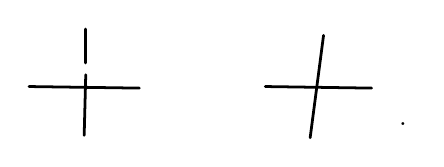
\begin{tikzpicture}[x=1cm,y=1cm,line width=1pt,line cap=round]
\draw (-.7,.02) -- (.7,0);
\draw (0,-.6) -- (.02,.17);
\draw (.02,.32) -- (.02,.75);
\draw (2.3,.02) -- (3.65,0);
\draw (2.87,-.63) -- (3.04,.67);
\node at (4.05,-.45) {.};
\end{tikzpicture}}}
\end{GelfandAdjacentEvidence}
\begin{GelfandAdjacentEvidence}{GELFAND-P000142}{3}

по 1-му растяг.\,[?], по другому сжимает ($\leq$, $\geq$ оценки на сжатие и растяжение)
\Unclear{GELFAND-P000142}{stretch-contraction}{Последняя буква сокращения после «по 1-му» имеет густые соединённые штрихи: «растяг.» / «растяж.». Сокращение не развёрнуто.}
\end{GelfandAdjacentEvidence}

\begin{center}
\begin{tikzpicture}[x=1cm,y=1cm]
\node[anchor=north west,inner sep=0pt,text width=.9\linewidth] (example) at (0,0) {\underline{Пример:} автом. тора, больше было неизвестно.\par Смейл утвержд., что нашёл мн-зия, кроме тора и их $U$-автом. и все такие автом. (гипотеза).};
\draw[line width=.6pt] ([xshift=-2mm]example.north west) -- ([xshift=-2mm]example.south west);
\draw[line width=.6pt] ([xshift=-3.5mm]example.north west) -- ([xshift=-3.5mm]example.south west);
\end{tikzpicture}
\end{center}

\uwave{Точное опр.:}\quad $\exists TM_x=X_x\oplus Y_x$, $\forall\xi\in X_x$, $g^*\xi\in X_{gx}$,
\par\noindent сущ. рим. метрика
\begin{gather*}
|g^*\xi|<\theta|\xi|,\quad 0<\theta<1,\\
\forall\eta\in Y_x,\quad |g^*\eta|>\frac1\theta|\eta|.
\end{gather*}

\begin{GelfandAdjacentEvidence}{GELFAND-P000142}{4}
(это $V$\,[?]-каскад)
\Unclear{GELFAND-P000142}{u-v-designation}{Начальный заголовок имеет $U$, а здесь знак похож на $V$: $V$-каскад / $U$-каскад.}
\end{GelfandAdjacentEvidence}

\uwave{Автом. тора} — соб. направления соотв. матрицы.

\begin{GelfandAdjacentEvidence}{GELFAND-P000142}{5}
Все
\begin{tikzpicture}[x=1cm,y=1cm,baseline=(cancel.base)]
\node (cancel) at (1.9,.55) {[зачёркнутое неразобранное слово]};
\node at (1.9,-.15) {новые примеры};
\draw[line width=.5pt] (-.1,-.35) .. controls (.03,.28) and (.3,.05) .. (.7,.12) -- (3.8,.12) .. controls (4.15,.1) and (4.2,-.1) .. (4.2,-.35);
\end{tikzpicture}
— фактор. ниль. группы по дискр. подгруппе. (ниль-Мн-зия)
\Unclear{GELFAND-P000142}{cancelled-examples-word}{Зачёркнутое слово после «Все» имеет с/ю/д-подобные остатки; исходное слово неразборчиво. Вставка «новые примеры» видима под охватывающей дугой.}
\end{GelfandAdjacentEvidence}
\begin{GelfandAdjacentEvidence}{GELFAND-P000142}{6}

$G/\Gamma$, $G=$
\begin{center}
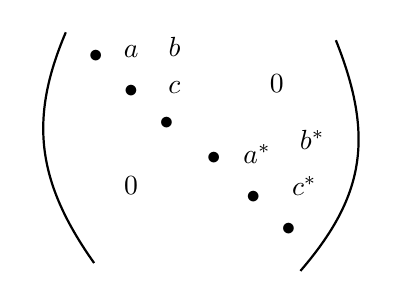
\begin{tikzpicture}[x=1cm,y=1cm]
\draw[line width=.8pt] (.12,2.95) .. controls (-.35,1.85) and (-.25,1.05) .. (.48,.02);
\draw[line width=.8pt] (3.55,2.85) .. controls (4.05,1.6) and (3.9,.85) .. (3.1,-.08);
\node at (.5,2.65) {$\bullet$};
\node at (.95,2.7) {$a$};
\node at (1.5,2.77) {$b$};
\node at (.95,2.2) {$\bullet$};
\node at (1.5,2.25) {$c$};
\node at (1.4,1.8) {$\bullet$};
\node at (2.8,2.3) {$0$};
\node at (.95,1) {$0$};
\node at (2,1.35) {$\bullet$};
\node at (2.55,1.4) {$a^*$};
\node at (3.25,1.58) {$b^*$};
\node at (2.5,.85) {$\bullet$};
\node at (3.15,1) {$c^*$};
\node at (2.95,.45) {$\bullet$};
\end{tikzpicture}
\end{center}
— 6-го порядка
\Unclear{GELFAND-P000142}{nilpotent-matrix}{Матрица в круглых скобках, шесть позиций на диагонали, два верхнетреугольных блока. Сверху $a,b$, ниже $c$; в нижнем блоке $a^*,b^*,c^*$; вне блоков два $0$. Шесть густых диагональных знаков показаны точками: $1$ / чёрные точки; точное буквальное чтение не установлено.}
\end{GelfandAdjacentEvidence}
\begin{GelfandAdjacentEvidence}{GELFAND-P000142}{7}

\begin{gather*}
\Gamma=\left\{\begin{aligned}
a&=m+n\sqrt3,\qquad a^{*\text{[?]}}=m-n\sqrt3\\
b&=m'+n'\sqrt3,\qquad \vcenter{\hbox{\begin{tikzpicture}[x=1cm,y=1cm,baseline=0pt,line width=1pt]
\draw (0,.08) -- (.05,0);
\draw (.45,.08) -- (.47,.01);
\draw (.88,.07) -- (.92,.02);
\draw (1.35,.08) -- (1.39,.01);
\draw (1.82,.1) -- (1.88,.03);
\draw (2.23,.11) -- (2.22,.05) -- (2.27,.02);
\end{tikzpicture}}},\\
c&=m''+n''\sqrt3,
\end{aligned}\right\}
\end{gather*}
\underline{$G/\Gamma$ компактно.}
\par Размерн. $3+3$
\par сжим. и расшир.
\Unclear{GELFAND-P000142}{lower-lattice-and-brace}{Над вторым $a$ короткий густой знак: звёздочка / штрих; $a^*$ дано с этой оговоркой. Справа от строки $b$ шесть повторительных коротких штрихов; их содержание не развёрнуто. Справа охватывающая фигурная скобка. Горизонтальная черта под «$G/\Gamma$ компактно.» проходит над «Размерн. $3+3$».}
\end{GelfandAdjacentEvidence}



\SourcePage{GELFAND-P000143}{unlabelled}
\underline{Собственно Аносов.}

Каскад — итерации дифф. гомеоморфизма
(с непр. временем — поток)
Описать типичные динамич. системы — каскады.
(всюду плотное мн-во, открытое)

\underline{Грубый поток} — перех. в экв. при малом $(C^1)$ возмущ.
(экв. — отлич. диффеом.)

\uwave{2-мерн. случай:} \underline{теор. Андронова-Понтрягина} — описаны грубые системы (конечн. число «устойч.» циклов и особ. точек и сепаратрисы сёдел в общем положении — — не пересек., не сов.) Их мн-во откр., плотное.

\uwave{Система Андронова-Понтрягина.}

1. Кон. число полож. равн. и периодич. траекторий, причём все они локально грубые (усл. на соб. знач. и мультипликаторы)
(многомерный случай это уже нетрив.)

2. Сепаратрисы общего положения

\noindent\begin{tabular}{p{.47\linewidth}p{.47\linewidth}}
(Усл.,\newline Условно устойч. мн-зия,\newline Асимпт. пучки,\newline орисферы,\newline орициклы) & (Мн-зия вход. и выходящих —\newline — см. Коддингтон и Левинсон)
\end{tabular}

3. Все траектории при $t\longrightarrow\pm\infty$ стремятся к полож. равновесия и периодич. решениям.

\begin{GelfandAdjacentEvidence}{GELFAND-P000143}{1}
[Две строки густо зачёркнуты прямыми и волнистыми линиями. Сохранились: $4)$ / $\forall$\,[?], «сепаратр. общего полож.», «(не пересек.», $2$\,[?], «собр.»; снизу «это не очень» [неразобранный конец].]
\Unclear{GELFAND-P000143}{cancelled-fourth-condition}{Начальный перечёркнутый знак $4)$- / $\forall$-подобный; далее сохранились «сепаратр. общего полож.», «(не пересек.», $2$-подобный знак и «собр.»; снизу «это не очень» и густой конец. Полное первоначальное высказывание неразборчиво.}
\end{GelfandAdjacentEvidence}

\underline{4 утверждения.}

\begin{GelfandAdjacentEvidence}{GELFAND-P000143}{2}
1. Все А.-П. — грубые —

\begin{tikzpicture}[x=1cm,y=1cm,baseline=(q.base)]
\node (q) at (0,0) {?};
\draw[line width=.7pt] (0,0) ellipse (.32cm and .4cm);
\end{tikzpicture}
\begin{center}
\begin{tikzpicture}[x=1cm,y=1cm]
\node[anchor=north west,inner sep=0pt,text width=.52\linewidth] (claims) at (0,0) {2. Все грубые — А.-П.\par 3. А.-П. плотны\par \sout{(дру\,[?]}\par 4. Грубые плотны};
\draw[line width=.7pt] ([xshift=3mm]claims.north east) -- ([xshift=3mm]claims.south east);
\draw[line width=.7pt] ([xshift=4.5mm]claims.north east) -- ([xshift=4.5mm]claims.south east);
\node[anchor=west,align=left] at ([xshift=10mm]claims.east) {Опровергнуты\\Смейлом.};
\end{tikzpicture}
\end{center}
\SourceFigure{GELFAND-P000143}{four-assertions}{После пункта 1 обведён крючкообразный вопросительный знак с отдельной точкой. Справа от пунктов 2–4 две вертикальные черты и надпись «Опровергнуты Смейлом».}
\end{GelfandAdjacentEvidence}

\begin{GelfandAdjacentEvidence}{GELFAND-P000143}{3}
\Unclear{GELFAND-P000143}{cancelled-parenthesis}{Короткая зачёркнутая скобка под пунктом 3: «дру» / «друг» / неразборчиво.}
\end{GelfandAdjacentEvidence}



\SourcePage{GELFAND-P000144}{7}
\begin{flushright}
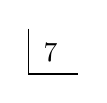
\begin{tikzpicture}[x=1cm,y=1cm,baseline=(p.base)]
\node (p) at (0,0) {$7$};
\draw[line width=.6pt] (-.28,.3) -- (-.28,-.28) -- (.35,-.28);
\end{tikzpicture}
\end{flushright}
\underline{Грубая система:} $\dot w=f(w)$.
\begin{equation*}
\forall\varepsilon\ \exists\delta,\quad \forall g,\quad \|g-f\|_{C^1}<\delta,
\end{equation*}
$\exists\varepsilon$-гомеом., перев. траект. $f$ в траект. $g$.

Для каскада: коммут. диагр

($\exists\varepsilon$-гомеом. $\chi$)

\begin{GelfandAdjacentEvidence}{GELFAND-P000144}{1}
\SourceFigure{GELFAND-P000144}{conjugacy-square}{Четыре $M$; сверху $f$, снизу $g$, обе горизонтальные стрелки вправо, обе вертикальные вниз. Слева $\chi$; справа короткий $x$- / $\chi$-подобный знак.\par\smallskip\centering{\color{black}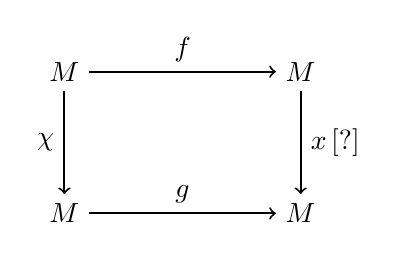
\begin{tikzpicture}[x=1cm,y=1cm]
\node (a) at (0,0) {$M$};
\node (b) at (3,0) {$M$};
\node (c) at (0,-1.8) {$M$};
\node (d) at (3,-1.8) {$M$};
\draw[->,line width=.7pt] (a) -- node[above] {$f$} (b);
\draw[->,line width=.7pt] (c) -- node[above] {$g$} (d);
\draw[->,line width=.7pt] (a) -- node[left] {$\chi$} (c);
\draw[->,line width=.7pt] (b) -- node[right] {$x\,[?]$} (d);
\end{tikzpicture}}}
\end{GelfandAdjacentEvidence}

(Для потоков естеств. считать, что может меняться скорость,
если это запретить, то грубых почти не остаётся)

\uwave{Подмн-во $b\vert$\,[?] мн-зия $M$ с гладк. каскадом наз.}
\uwave{$U$-подмн-вом}
(\underline{гиперболическое} \underline{подмн-во})

компактно,

инвариантно,

\begin{GelfandAdjacentEvidence}{GELFAND-P000144}{2}
$\exists\Theta$ и разб. кас. пучка над $b\vert$\,[?] в прямую сумму,
облад. указ. св-вами. ($U$ $\ldots$)
\Unclear{GELFAND-P000144}{hyperbolic-set-symbol}{Обозначение подмножества: $b\vert$ / $b_1$ / иной знак; петля и отдельная высокая черта. Повторено после «над».}
\end{GelfandAdjacentEvidence}
\begin{GelfandAdjacentEvidence}{GELFAND-P000144}{3}

(кас. пр-во всего [зачёркнут неразборчивый короткий фрагмент] мн-зия разбив.)
\Unclear{GELFAND-P000144}{cancelled-tangent-word}{После «всего» густо зачёркнут короткий фрагмент; буквальное слово не читается.}
\end{GelfandAdjacentEvidence}

\underline{Пример:} 1) гиперболич. полож. равновесия
(напр. устойч. — — расшир. — всё пр-во)

2) любая $U$-система

3) Есть примеры, когда такое мн-во тор, канторово и т.д.

\underline{Системы Смейла.}

\uwave{Неблуждающая точка.}

\begin{GelfandAdjacentEvidence}{GELFAND-P000144}{4}
\uwave{Блужд. область:} $\exists n_0$, что
\begin{equation*}
\forall n\ge n_0,\quad g^n U\cap U=\varphi\,[?]
\end{equation*}
\Unclear{GELFAND-P000144}{wandering-zero-and-headings}{Справа от равенства перечёркнутый овал с длинным нижним штрихом: $\varphi$- / $\varnothing$-подобный знак. «Системы Смейла» подчёркнуто прямой чертой, два следующих заголовка — волнистой.}
\end{GelfandAdjacentEvidence}

Точка наз. блужд., если она имеет блужд. окрестность.

\begin{GelfandAdjacentEvidence}{GELFAND-P000144}{5}
Неблужд. точка — точка, не явл. блужд., т.е.
\begin{equation*}
\forall U_p\ \forall n\quad \exists g\,[?]\in U_p,\quad m>n:\quad g^m q\in U_p.
\end{equation*}
\Unclear{GELFAND-P000144}{nonwandering-point-variable}{После $\exists$ стоит $g$- / $q$-подобная буква; в конце после $g^m$ — $q$-подобная.}
\end{GelfandAdjacentEvidence}

\underline{Мн-во неблужд. точк замкнуто.} (обозн. — $\Omega$)

\uwave{Система} \uwave{Смейла} (def)

1. $\Omega$ — гиперболическое.

\begin{GelfandAdjacentEvidence}{GELFAND-P000144}{6}
2. $\overline{\Gamma}=\Omega$
(периодич. точки плотны в $\Omega$ — неблужд.\,[?])
\Unclear{GELFAND-P000144}{bottom-parenthesis}{Конец пояснения у нижней границы: «— неблужд.» / сходное сокращение; густые штрихи.}
\end{GelfandAdjacentEvidence}
\begin{GelfandAdjacentEvidence}{GELFAND-P000144}{7}

\uwave{$\Gamma_n$ — мн-во точек периода $n$.}
\begin{equation*}
\vcenter{\hbox{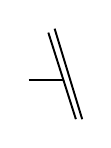
\begin{tikzpicture}[x=1cm,y=1cm]
\draw[line width=.7pt] (0,1.1) -- (.35,0);
\draw[line width=.7pt] (.08,1.15) -- (.43,0);
\draw[line width=.7pt] (-.25,.5) -- (.2,.5);
\end{tikzpicture}}}
\quad\Gamma=\bigcup_{n\ge1}\Gamma_n\,[?]\quad(g^n p=p)\,[?]
\end{equation*}
\Unclear{GELFAND-P000144}{periodic-definition-overwrite}{После знака объединения густо переписаны $\Gamma_n$-подобные знаки, начало скобки и $g$; показатель $n$-подобный. Первоначальные переписанные знаки не установлены. Слева две наклонные черты с короткой поперечной чертой.}
\end{GelfandAdjacentEvidence}



\begin{GelfandAdjacentEvidence}{GELFAND-P000145}{1}
\SourcePage{GELFAND-P000145}{unlabelled}
Бывает, что все точки неблужд., а периодич. нет
(напр. ниль-потоки\,[?])
\Unclear{GELFAND-P000145}{initial-example}{Слабая запись в скобках: «ниль-потоки» / «нуль-потоки»; средняя буква не вполне ясна.}
\end{GelfandAdjacentEvidence}
\begin{GelfandAdjacentEvidence}{GELFAND-P000145}{2}

\underline{Гипотезы.}
\begin{center}
\begin{tikzpicture}[x=1cm,y=1cm]
\node[anchor=north west,inner sep=0pt,text width=.92\linewidth] (hyp) at (0,0) {$\{\overline{\Gamma}=\Omega\}$ — всюду плотны — доказана [Гото / Пью / Гью?]; 1964};
\node[anchor=north west,inner sep=0pt] (c1) at ([xshift=-.32\linewidth,yshift=-3mm]hyp.south east) {(только в $C^1$)\quad!!};
\draw[line width=.6pt] ([xshift=-2mm,yshift=-1mm]hyp.south west) -- ([xshift=-2mm,yshift=2mm]c1.north west) -- ([xshift=-2mm,yshift=-1mm]c1.south west) -- ([yshift=-1mm]c1.south east);
\end{tikzpicture}
\end{center}
\Unclear{GELFAND-P000145}{proof-name}{Фамилия перед «; 1964»: «Гото» / «Пью» / «Гью»; слабое начертание.}
\end{GelfandAdjacentEvidence}

\uwave{Сист. Смейла всюду плотны}

\begin{tikzpicture}[x=1cm,y=1cm,baseline=(q.base)]
\node (q) at (0,0) {?};
\draw[line width=.6pt] (0,0) ellipse (.3cm and .38cm);
\end{tikzpicture}

Великая проблема, которой стоит посвятить жизнь.

Видимо 2 следует из 1 (Вероятн. $70\%$),
так что дост. док., что сист. с гиперб. $\Omega$ плотны.

\begin{GelfandAdjacentEvidence}{GELFAND-P000145}{3}
\underline{Теорема S.D.T.\,[?]} (Смейл) (Spectral Decompositio\,[?] theorem)
\Unclear{GELFAND-P000145}{spectral-initials}{Первая буква $S$-образная, средняя петлеобразная $D$ / «Д», последняя $T$-образная: S.D.T. / S.Д.T.}
\end{GelfandAdjacentEvidence}

\begin{GelfandAdjacentEvidence}{GELFAND-P000145}{4}
\Unclear{GELFAND-P000145}{spectral-title-terminal}{Конец слова перед «theorem»: Decompositio / Decomposition; последний видимый знак $o$- / $a$-подобный. Дополнительная конечная буква $n$ не установлена.}
\end{GelfandAdjacentEvidence}

\underline{о строении сист. Смейла.}
\begin{equation*}
\Omega=\bigcup_{i=1}^{k}\Omega_i
\end{equation*}
$\Omega_i$ — инв., замкнуты и топологически транзитивны.

Все теор. вытекают лишь из 1.



\SourcePage{GELFAND-P000146}{unlabelled}
$12/\underline{\overline{\mathrm{IX}}}$ \underline{Сем. Гельфанда.}

\begin{tikzpicture}[x=1cm,y=1cm,baseline=(sh.base)]
\node[anchor=south west,inner sep=0pt] (sh) at (0,.12) {Г.Е. Шилов.};
\draw[line width=.6pt] (0,0) .. controls (.16,.12) and (.25,-.12) .. (.4,0) .. controls (.56,.12) and (.65,-.12) .. (.8,0) .. controls (.96,.12) and (1.05,-.12) .. (1.2,0) .. controls (1.36,.12) and (1.45,-.12) .. (1.6,0) .. controls (1.76,.12) and (1.85,-.12) .. (2,0) .. controls (2.16,.12) and (2.25,-.12) .. (2.4,0) .. controls (2.56,.12) and (2.65,-.12) .. (2.8,0) .. controls (2.96,.12) and (3.05,-.12) .. (3.2,0);
\draw[line width=.6pt] (0,-.12) .. controls (.16,0) and (.25,-.24) .. (.4,-.12) .. controls (.56,0) and (.65,-.24) .. (.8,-.12) .. controls (.96,0) and (1.05,-.24) .. (1.2,-.12) .. controls (1.36,0) and (1.45,-.24) .. (1.6,-.12) .. controls (1.76,0) and (1.85,-.24) .. (2,-.12) .. controls (2.16,0) and (2.25,-.24) .. (2.4,-.12) .. controls (2.56,0) and (2.65,-.24) .. (2.8,-.12) .. controls (2.96,0) and (3.05,-.24) .. (3.2,-.12);
\end{tikzpicture}
\begin{equation*}
S=\{x\in H,\ |x|\le1\}
\end{equation*}
— ед. шар гильб. пр-ва.

$L(S)$ — кольцо всех слабо непр. функций.
\begin{equation*}
L(S)\subset\overline R\subset C(S)
\end{equation*}
$C(S)$ — сильно непр. ф-и.

\begin{GelfandAdjacentEvidence}{GELFAND-P000146}{1}
\begin{equation*}
R=\{f((e_1,x),\ldots,(e_n,x),|x-a_1|,\ldots,|x-a_m|),
\end{equation*}
$\overline R$ — замыкание
\Unclear{GELFAND-P000146}{ring-closing-brace}{После длинной формулы $R$ видны закрывающая круглая скобка и запятая; закрывающая фигурная скобка для начального $\{$ не видна.}
\end{GelfandAdjacentEvidence}
\begin{GelfandAdjacentEvidence}{GELFAND-P000146}{2}

\begin{center}
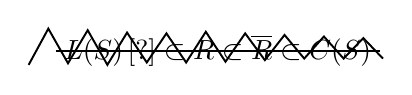
\begin{tikzpicture}[x=1cm,y=1cm]
\node[inner sep=0pt] (chain) at (0,0) {$L(S)\,[?]\subset R\subset\overline R\subset C(S)$};
\draw[line width=.7pt] ([xshift=-1mm]chain.west) -- ([xshift=1mm]chain.east);
\draw[line width=.7pt] (-2.4,-.18) -- (-2.15,.28) -- (-1.9,-.16) -- (-1.65,.26) -- (-1.4,-.18) -- (-1.15,.23) -- (-.9,-.15) -- (-.65,.22) -- (-.4,-.15) -- (-.15,.24) -- (.1,-.14) -- (.35,.22) -- (.6,-.12) -- (.85,.2) -- (1.1,-.1) -- (1.35,.18) -- (1.6,-.1) -- (1.85,.16) -- (2.1,-.1);
\end{tikzpicture}
\end{center}
\Unclear{GELFAND-P000146}{cancelled-inclusions}{Зачёркнута цепочка $L(S)\subset R\subset\overline R\subset C(S)$; первые буквы и первый знак включения переписаны, начало не вполне установлено.}
\end{GelfandAdjacentEvidence}

ПИМ кольца $L(S)$ — гильбертов шар

\begin{GelfandAdjacentEvidence}{GELFAND-P000146}{3}
ПИМ $\overline R$ — бикомп. расширение.
\begin{equation*}
M_\tau(f(x),z)\qquad M_\tau^*(f(x),z)
\end{equation*}
\Unclear{GELFAND-P000146}{mean-radius-symbol}{Индекс среднего $\tau$- / $r$-подобный; такой же петлеобразный знак в последующей формуле предела и в квадрате в знаменателе.}
\end{GelfandAdjacentEvidence}

$e_1,e_2,\ldots,e_n,\ldots$ — ортог. базис, опр. возраст. цепочку подпр-в $E_1\subset E_2\subset\ldots$
\begin{center}
\begin{tikzpicture}[x=1cm,y=1cm]
\node (sphere) at (0,0) {по сфере};
\node (ball) at (5,0) {по шару};
\draw[line width=.6pt] (0,0) ellipse (1.15cm and .34cm);
\draw[line width=.6pt] (5,0) ellipse (1.15cm and .34cm);
\end{tikzpicture}
\end{center}
Средние — предел конечномерных. Если сущ., то равны.

На $\overline R$ средние определены.

(Для $R$ можно просто написать ф-мы).

$M_\tau$ — мульт. функционал. Это max идеал, но он не есть знач. в точке, а знач. в бикомп. расширениях.

\begin{GelfandAdjacentEvidence}{GELFAND-P000146}{4}
Из т. $z$ пров. линии $M_\tau(z)$ в пр-ве max идеалов.
\begin{equation*}
\Delta f(z)=\lim_{\tau\to0}\frac{M_\tau[f(x),z]-f(z)}{\tau^2}.
\end{equation*}
\begin{flushright}
\begin{tikzpicture}[x=1cm,y=1cm]
\node[anchor=west,align=left,inner sep=0pt] (note) at (0,0) {втыкаются\\в точку $z$.};
\draw[line width=.7pt] ([xshift=-3mm,yshift=1mm]note.north west) -- ([xshift=-3mm,yshift=-1mm]note.south west);
\draw[line width=.7pt] ([xshift=-4.5mm,yshift=1mm]note.north west) -- ([xshift=-4.5mm,yshift=-1mm]note.south west);
\end{tikzpicture}
\end{flushright}
\Unclear{GELFAND-P000146}{limit-radius-repeat}{Петлеобразный знак в $M_\tau$, под пределом и в $\tau^2$ — $\tau$ / $r$ / неустановленная буква. Справа от формулы две вертикальные черты и «втыкаются в точку $z$».}
\end{GelfandAdjacentEvidence}

\underline{Это опер. 1-го порядка!!}
\begin{equation*}
\Delta(fg)=f\cdot\Delta g+(\Delta f)g
\end{equation*}

\underline{Зад. Дирихле.}

$\Sigma$ — $\underset{\text{(слаб)}}{\text{замкн. пов.}}$ (звёздная)

\begin{GelfandAdjacentEvidence}{GELFAND-P000146}{5}
\SourceFigure{GELFAND-P000146}{dirichlet-surface}{Неровный замкнутый округлый контур с $\Sigma$ справа сверху; семь расходящихся штрихов, с небольшими просветами у центра. Несколько проходят за контур, нижний левый заканчивается внутри; левый штрих изгибается перед центром. Нижний правый утолщён у контура; самостоятельная стрелка / точка не установлена.\par\smallskip\centering{\color{black}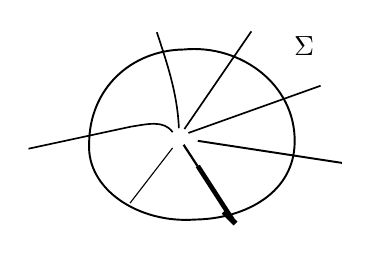
\begin{tikzpicture}[x=1cm,y=1cm]
\draw[line width=.7pt] (-1.18,-.12) .. controls (-1.18,.58) and (-.65,1.07) .. (.02,1.08) .. controls (.75,1.15) and (1.44,.63) .. (1.43,-.09) .. controls (1.43,-.72) and (.83,-1.07) .. (.16,-1.08) .. controls (-.56,-1.13) and (-1.21,-.69) .. (-1.18,-.12) -- cycle;
\draw[line width=.6pt] (-.04,.08) .. controls (-.06,.54) and (-.2,.93) .. (-.32,1.3);
\draw[line width=.6pt] (.03,.07) -- (.88,1.31);
\draw[line width=.6pt] (.08,.02) -- (1.76,.62);
\draw[line width=.7pt] (.2,-.08) -- (2.03,-.36);
\draw[line width=.8pt] (.02,-.13) -- (.64,-1.08);
\draw[line width=1.7pt] (.2,-.4) -- (.64,-1.08);
\draw[line width=2pt] (.53,-.98) -- (.68,-1.13);
\draw[line width=.4pt] (-.12,-.17) -- (-.66,-.87);
\draw[line width=.6pt] (-.12,.03) .. controls (-.23,.19) and (-.45,.13) .. (-.65,.1) -- (-1.95,-.18);
\node at (1.55,1.12) {$\Sigma$};
\end{tikzpicture}}}
\end{GelfandAdjacentEvidence}

\begin{gather*}
\Delta u(x)=0,\\
u(x)|_{x=\sigma}=f(\sigma)
\end{gather*}



\SourcePage{GELFAND-P000147}{10}
\begin{flushright}
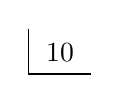
\begin{tikzpicture}[x=1cm,y=1cm,baseline=(p.base)]
\node (p) at (0,0) {$10$};
\draw[line width=.6pt] (-.4,.3) -- (-.4,-.28) -- (.4,-.28);
\end{tikzpicture}
\end{flushright}
Есть единств. и непр. зависимость для $f\in\overline R$ и поверхн. вида
\begin{equation*}
\sum_{k=m+1}^{\infty}\xi_k^2=\varphi(\xi_1,\ldots,\xi_m)
\end{equation*}

\begin{GelfandAdjacentEvidence}{GELFAND-P000147}{1}
(пов. вращ.) вокруг подпр-ва [зачёркнут короткий неразборчивый фрагмент] кон. коразмерн.
\Unclear{GELFAND-P000147}{cancelled-margin}{Перед «кон. коразмерн.» густо зачёркнут короткий фрагмент; буквальное слово не установлено.}
\end{GelfandAdjacentEvidence}

и огранич. кривизна.

Ф-ла решения — угловое среднее от гран. функционала.

$\Delta u=g\in\overline R$ — тоже явная

Далее $\Delta u=\varphi(x,u(x))$ решается методом неподв. точки.

\begin{tikzpicture}[x=1cm,y=1cm,baseline=(gh.base)]
\node[anchor=south west,inner sep=0pt] (gh) at (0,.15) {И.М. Гельфанд.};
\draw[line width=.6pt,domain=0:4,samples=65] plot (\x,{.05*sin(720*\x)});
\draw[line width=.6pt,domain=0:4,samples=65] plot (\x,{-.12+.05*sin(720*\x)});
\end{tikzpicture}

\begin{GelfandAdjacentEvidence}{GELFAND-P000147}{2}
$u=(u_1,\ldots,u_m\,[?])$
\Unclear{GELFAND-P000147}{component-count-index}{Последний индекс компоненты имеет $m$- / $n$-подобное густое начертание; ниже отдельно написано $n=1$ и $n=2$.}
\end{GelfandAdjacentEvidence}

\begin{equation*}
\frac{\partial u}{\partial t}=A(u)\frac{\partial u}{\partial x}
\end{equation*}
Гиперболична ($\forall$ точке $A(u)$ имеет веществ. собств. знач.)

Есть ли единств.? Ударные волны — реш. может быть неод.

$n=1$ — всегда единств., если $f(u)$ — выпукла

\begin{GelfandAdjacentEvidence}{GELFAND-P000147}{3}
Ур-я гидродинамики — [зачёркнуто: «неод.» / «может» / неразборчиво] тоже единств. ($n=2$)
\Unclear{GELFAND-P000147}{hydro-cancelled-word}{Перед «тоже единств.» зачёркнуто слово: «может» / «неод.» / иной короткий фрагмент; перечёркивание проходит через буквы.}
\end{GelfandAdjacentEvidence}

В общем случае неясно, \dashuline{где есть единств. и где нет}.

\begin{GelfandAdjacentEvidence}{GELFAND-P000147}{4}
Магн.\,[?] гидродин. — тоже единств.
\Unclear{GELFAND-P000147}{hydro-prefix}{Первое сокращение перед «гидродин.»: «Магн.» / «Мал.»; штрихи после «Ма» соединены.}
\end{GelfandAdjacentEvidence}

\uwave{Чисто матем. вопрос:} $\forall$ точке $u$ нарисуем собств. вектора — 3 сем-ва линий — — характеристики.

Выпуклость: возможно, рост $\lambda$ по характеристикам

Лучше:
\begin{equation*}
\frac{\partial u}{\partial t}=\frac{\partial f(u)}{\partial x}
\end{equation*}
(дивергентный вид)

Есть раб. Годунова, но там узкий класс систем.

Когда есть единств. при доб. вязкости:
\begin{equation*}
\frac{\partial u}{\partial t}=A\frac{\partial u}{\partial x}+\varepsilon\frac{\partial^2u}{\partial x^2}\quad?
\end{equation*}

\begin{GelfandAdjacentEvidence}{GELFAND-P000147}{5}
Это сводится к [зачёркнуто неразборчивое слово] вопросу обыкн. дифф. уравнений.
\Unclear{GELFAND-P000147}{cancelled-final-word}{Между «к» и «вопросу» густое зачёркнутое слово с нижним петлеобразным штрихом; буквальное чтение не установлено.}
\end{GelfandAdjacentEvidence}



\SourcePage{GELFAND-P000148}{unlabelled}
\begin{tikzpicture}[x=1cm,y=1cm,baseline=(bh.base)]
\node[anchor=south west,inner sep=0pt] (bh) at (0,.15) {И. Бернштейн.};
\draw[line width=.6pt,domain=0:4,samples=65] plot (\x,{.05*sin(720*\x)});
\draw[line width=.6pt,domain=0:4,samples=65] plot (\x,{-.12+.05*sin(720*\x)});
\end{tikzpicture}

Часть того, что рассказывал \underline{Атийя}.

$g$ — комп. группа Ли. $R_g$ — кольцо конечномерных предст.
(прям. сумма, тенз. произв. и формальные разности), коммутативное.

Вложение
\begin{equation*}
R_g\longrightarrow K(B_g)
\end{equation*}
$B_g$ — классиф. пр-во,
$K$ — $K$-функтор.

Представлению соотв. векторное расслоение на $B_g$ (ассоциированное).


\begin{tikzpicture}[x=1cm,y=1cm,baseline=(ci.base)]
\node (ci) at (0,0) {$\mathrm{I.}$};
\draw[line width=.7pt] (0,0) ellipse (.33cm and .36cm);
\end{tikzpicture}
Если пополнить кольцо $R_g$ по идеалу представлений нулевой размерности, то будет изоморфизм
\begin{equation*}
\widehat R_g\longrightarrow k(B_g)
\end{equation*}
(Разм. элемента вида разности двух предст. — разность размерностей)

\underline{Пример.}
\begin{equation*}
g=S^1,\qquad R_{S^1}=\sum_{i=-\infty}^{+\infty}n_i x^i,
\end{equation*}
$n_i$ — целые, конечн. число ненулевых.

Идеал порожд. элементом $x-1=y$.

\begin{equation*}
\widehat R_{S^1}=Z[[y]]
\end{equation*}
(форм. степ. ряды)

Степени только положительные
\begin{equation*}
\left(\frac1{1-y}=1+y+y^2+\ldots\right)
\end{equation*}
\begin{gather*}
B_g=CP^\infty,\\
k(CP^\infty)=\lim K(CP^n).
\end{gather*}

На $CP^n$ канонич. расслоение (слой $CP^1$), пр-во $CP^{n+1}$.

Всякий элем. $K(CP^n)$ есть $\underline{P}(x-1)$.

\begin{GelfandAdjacentEvidence}{GELFAND-P000148}{1}
Точно
\begin{equation*}
K(CP^n)\cong\,[?]\ P(x)/(x-1)^{n+1}.
\end{equation*}
\Unclear{GELFAND-P000148}{quotient-relation}{Знак отношения с волнистым верхом и нижними горизонтальными штрихами: $\cong$ / $\simeq$ / переписанный знак. В числителе $P$-образная буква.}
\end{GelfandAdjacentEvidence}

В следующий раз лекция Минлоса по стат. физике.



\SourcePage{GELFAND-P000149}{unlabelled}
19/$\overline{\underline{\mathrm{IX}}}$. \uwave{Сем. Гельфанда.}

\uwave{И. Бернштейн} (продолжение).

$K(B_g)$ определяется так:

Пусть
\begin{gather*}
(B_g)_1\longrightarrow(B_g)_2\longrightarrow\ldots
\end{gather*}
остовы соотв. размерности
\begin{gather*}
K_1\longleftarrow K_2\longleftarrow\ldots
\end{gather*}
Надо взять проект. предел.

\begin{GelfandAdjacentEvidence}{GELFAND-P000149}{1}
$K$-функтор конечного полиэдра опред. обычным образом
(кольцо [переписано: $K$-подобный знак, ?] рассл.[?])
\sout{[неразобранная длинная запись]}) .
\begin{center}
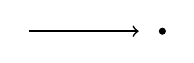
\begin{tikzpicture}[x=1cm,y=1cm]
\draw[->,line width=.6pt] (0,0)--(1.4,0);
\fill (1.7,0) circle (.045cm);
\end{tikzpicture}
\end{center}
\Unclear{GELFAND-P000149}{cancelled-definition}{После «кольцо» переписанный $K$-подобный знак и «рассл.»-подобное сокращение. Далее густое зачёркивание с нижними штрихами и ещё одной закрывающей скобкой; под началом зачёркивания стрелка вправо и точка. Буквальное чтение зачёркнутого окончания не установлено.}
\end{GelfandAdjacentEvidence}
\begin{GelfandAdjacentEvidence}{GELFAND-P000149}{2}

\uwave{Вопрос И.М. Гельфанда.} обобщить понятие $K$-функтора
и классиф. пр-ва, чтобы сохр. теорема и для лок.
компактных групп Ли. (лев. часть имеет смысл) —
— надо исп. и бесконечномерные предст.
\SourceFigure{GELFAND-P000149}{question-parenthesis}{Под заголовком волнистая линия. Слабая запись в скобках: «лев. часть имеет смысл»; справа предыдущей строки «лок.».}
\end{GelfandAdjacentEvidence}
\begin{GelfandAdjacentEvidence}{GELFAND-P000149}{3}

Размерность — множитель[?] в ф-ле Планшереля.
\begin{center}
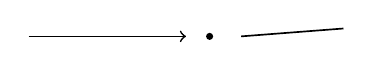
\begin{tikzpicture}[x=1cm,y=1cm]
\draw[->,line width=.6pt] (0,0)--(2,0);
\fill (2.3,0) circle (.045cm);
\draw[line width=.6pt] (2.7,0)--(4,.1);
\end{tikzpicture}
\end{center}
\Unclear{GELFAND-P000149}{plancherel-comparison}{Связанное слово после тире: «множитель» / «показатель» / неясная запись. Под ним длинная стрелка вправо, точка и короткий слегка восходящий штрих.}
\end{GelfandAdjacentEvidence}

Пусть $X$ — $g$-пространство
(т.е. есть отображение $g\times X\longrightarrow X$,
непр. по обоим аргументам и есть
действие $g$ на $X$)

\begin{GelfandAdjacentEvidence}{GELFAND-P000149}{4}
$K_g(X\,[?])$ — $K_g$[?]-функтор.
\Unclear{GELFAND-P000149}{functor-index-placement}{У второго $K$ малые петлеобразные штрихи справа выше и ниже: $K_g$ / $K^g$ / $K_g^0$-подобная запись; отдельный $0$ не установлен. В скобках первого $K_g$ густо переписана $X$-подобная буква.}
\end{GelfandAdjacentEvidence}

$g$-пучок $E\overset p\longrightarrow X$ — вект. пучок, то $E$ ...
— $g$-пр-во, $g$ действует согласованно с $p$.
В слоях $g$ должно сохранять линейную структуру.

Обычн. образом опр. сумма, тенз. произв. и ввод.
формальные разности.

\underline{Пример.} $K_g$ — функтор точки —
— лин. пр-ва с предст. $g$,
это будет в точности $R_g$.

\begin{GelfandAdjacentEvidence}{GELFAND-P000149}{5}
\sout{Н[?]...}
\Unclear{GELFAND-P000149}{cancelled-generalization}{Перед «Обобщение» короткий зачёркнутый фрагмент с Н-образным началом; остальные буквы не установлены.}
\end{GelfandAdjacentEvidence}

\underline{Обобщение.} Вместо точки — $g$-пр-во $X$.

Левая часть $K_g(X)$ — уже обобщена.

\begin{GelfandAdjacentEvidence}{GELFAND-P000149}{6}
\begin{center}
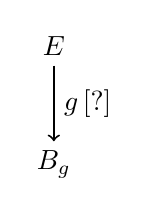
\begin{tikzpicture}[x=1cm,y=1cm]
\node (be) at (0,1.5) {$E$};
\node (bb) at (0,0) {$B_g$};
\draw[->,line width=.7pt] (be.south)--node[right] {$g\,[?]$} (bb.north);
\end{tikzpicture}
\end{center}
$E$ — $g$-пр-во ($g$ действ. справа).
\Unclear{GELFAND-P000149}{bottom-bundle}{Внизу $E$ над $B_g$, стрелка вниз, справа малый $g$-подобный петлеобразный знак; точное чтение метки не установлено.}
\end{GelfandAdjacentEvidence}



\clearpage

\begin{GelfandAdjacentEvidence}{GELFAND-P000150}{1}
\SourcePage{GELFAND-P000150}{14}
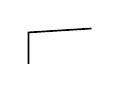
\begin{tikzpicture}[x=1cm,y=1cm,baseline=0pt]
\draw[line width=.6pt] (0,0)--(0,.4)--(.8,.45);
\end{tikzpicture}
\hfill\begin{tikzpicture}[x=1cm,y=1cm,baseline=(pn.base)]
\node (pn) at (.35,.35) {$14$};
\draw[line width=.6pt] (0,.85)--(0,0)--(1.05,0);
\end{tikzpicture}

Пусть $X$ — $G\,[?]$-пр-во. Введём пр-во $X_G=E\times_G X$
(в $E\times X$ склеены орбиты группы $G$).
Если $X$ — точка, то $X_G\cong B_G$ — Грассман.

\Unclear{GELFAND-P000150}{group-glyph}{Петлеобразный знак группы и повторяющиеся индексы: $G$ / $g$ / $\mathcal G$; начертание передано как $G$ с этой оговоркой.}
\end{GelfandAdjacentEvidence}

\uuline{Теорема.} (обобщение вначале формулированной)
\begin{equation*}
\widehat K_G(X)\overset{\sim}{\longrightarrow}K(X_G).
\end{equation*}
Есть отобр. $K_G(*)\longrightarrow K_G(X)$, поэтому $K_G(X)$ —
— модуль над $R_G$. Пополнение берётся по идеалу $J$
кольца $R_G$.

Точное опр. можно дать и так:
\begin{equation*}
\widehat K_G(X)=K_G(X)\underset{R_G}{\otimes}\widehat R_G.
\end{equation*}
\begin{center}
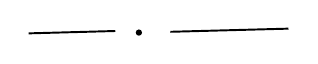
\begin{tikzpicture}[x=1cm,y=1cm]
\draw[line width=.7pt] (0,0)--(1.1,.03);
\fill (1.4,.01) circle (.04cm);
\draw[line width=.7pt] (1.8,.02)--(3.3,.06);
\end{tikzpicture}
\end{center}
1. \dashuline{Редукция к унитарной группе $U$.}

Пусть $G\subset U$.
Тогда $K_G(X)=K_U(U\times_G X)$.

Действие $G$ на $U$: $g:u\longrightarrow ug^{-1}$.
На $U\times_G X$ действует $U$ слева.
Кроме того, $X_G=(U\times_G X)_U$.
\begin{flushright}
\begin{tikzpicture}[x=1cm,y=1cm]
\node[anchor=north west,inner sep=0pt,text width=.30\linewidth] (sidebar) at (0,0) {Видно, почему\par нельзя\par ограничиться\par такой};
\draw[line width=.7pt] ([xshift=-2mm]sidebar.north west)--([xshift=-2mm]sidebar.south west);
\draw[line width=.7pt] ([xshift=-3.5mm]sidebar.north west)--([xshift=-3.5mm]sidebar.south west);
\end{tikzpicture}
\end{flushright}

2. \dashuline{Сведение к случаю тора.}

\begin{GelfandAdjacentEvidence}{GELFAND-P000150}{2}
(Для тора верна, т.к. для окр. пров.\,[?] непосредств.)
\Unclear{GELFAND-P000150}{torus-parenthesis}{После «окр.» сокращение, похожее на «пров.» / «пр-в.»; соединённые средние штрихи. В скобке слово «непосредств.». }
\end{GelfandAdjacentEvidence}
\begin{GelfandAdjacentEvidence}{GELFAND-P000150}{3}

\sout{[неразобранный зачёркнутый знак]}.
\Unclear{GELFAND-P000150}{cancelled-torus-number}{Перед $T\subset U$ густо зачёркнут короткий номероподобный знак; первоначальное чтение не установлено. Справа отдельная точка.}
\end{GelfandAdjacentEvidence}
\begin{GelfandAdjacentEvidence}{GELFAND-P000150}{4}

$T\subset U$, $T$ — максимальный тор в $U$.
\begin{center}
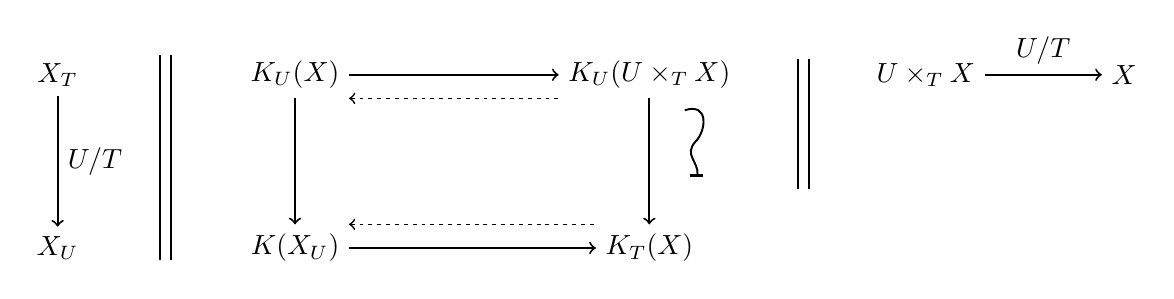
\begin{tikzpicture}[x=.9cm,y=1cm]
\node (fibreT) at (.35,0) {$X_T$};
\node (fibreU) at (.35,-2.2) {$X_U$};
\draw[->,line width=.7pt] (fibreT.south)--node[right] {$U/T$} (fibreU.north);
\draw[line width=.7pt] (1.8,.25)--(1.8,-2.35);
\draw[line width=.7pt] (1.95,.25)--(1.95,-2.35);
\node (topA) at (3.7,0) {$K_U(X)$};
\node (topB) at (8.7,0) {$K_U(U\times_T X)$};
\node (bottomA) at (3.7,-2.2) {$K(X_U)$};
\node (bottomB) at (8.7,-2.2) {$K_T(X)$};
\draw[->,line width=.7pt] (topA.east)--(topB.west);
\draw[<-,dash pattern=on 1.4pt off 1.8pt,line width=.6pt] ([yshift=-3mm]topA.east)--([yshift=-3mm]topB.west);
\draw[->,line width=.7pt] (bottomA.east)--(bottomB.west);
\draw[<-,dash pattern=on 1.4pt off 1.8pt,line width=.6pt] ([yshift=3mm]bottomA.east)--([yshift=3mm]bottomB.west);
\draw[->,line width=.7pt] (topA.south)--(bottomA.north);
\draw[->,line width=.7pt] (topB.south)--(bottomB.north);
\draw[line width=.7pt] (9.2,-.45) .. controls (9.55,-.35) and (9.5,-.72) .. (9.35,-.85) .. controls (9.18,-1.02) and (9.4,-1.1) .. (9.38,-1.28);
\draw[line width=1.3pt] (9.28,-1.28)--(9.45,-1.28);
\draw[line width=.7pt] (10.8,.2)--(10.8,-1.45);
\draw[line width=.7pt] (10.95,.2)--(10.95,-1.45);
\node (projectionA) at (12.6,0) {$U\times_T X$};
\node (projectionB) at (15.4,0) {$X$};
\draw[->,line width=.7pt] (projectionA.east)--node[above] {$U/T$} (projectionB.west);
\end{tikzpicture}
\end{center}
\SourceFigure{GELFAND-P000150}{torus-diagrams}{Слева $X_T\longrightarrow X_U$ вниз с $U/T$. Две двойные вертикальные черты разделяют три части. В квадрате сверху $K_U(X)$ и $K_U(U\times_T X)$, снизу $K(X_U)$ и $K_T(X)$; сплошные горизонтальные стрелки вправо, пунктирные обратно, обе вертикальные вниз. Справа от правой вертикали вопросоподобный крючок с утолщённым низом; отдельная точка не выделяется. Справа отдельно $U\times_T X\longrightarrow X$ с $U/T$ над стрелкой.}
\end{GelfandAdjacentEvidence}

Верхняя стрелка — отобр. в прямое \underline{слагаемое} (т.е. сущ.
\begin{tikzpicture}[x=1cm,y=1cm,baseline=(inverse.base)]
\node[anchor=base west,inner sep=0pt] (inverse) at (0,0) {„обратное};
\node[anchor=south west,inner sep=0pt,font=\small] at (0,.34) {(и нечётное\,[?])};
\end{tikzpicture}
строится сверху и снизу функториально. \underline{„обратное“})

\begin{GelfandAdjacentEvidence}{GELFAND-P000150}{5}
Отсюда левая стрелка тоже изоморфизм.
\Unclear{GELFAND-P000150}{inverse-insert}{Над первым «обратное» вставка в скобках: «и нечётное» / «и нечётн.» / «и нечёткое» / «и нечётная» / густое сокращение после «и». Средние и конечные штрихи не разделяются уверенно. Подчёркнуты «слагаемое» и последнее «обратное».}
\end{GelfandAdjacentEvidence}



\begin{GelfandAdjacentEvidence}{GELFAND-P000151}{1}
\SourcePage{GELFAND-P000151}{unlabelled}
\begin{tikzpicture}[x=1cm,y=1cm,baseline=(minlos.base)]
\node[inner sep=0pt,outer sep=0pt] (minlos) {Р.А. Минлос};
\begin{scope}
\clip ([yshift=-2pt]minlos.south west) rectangle ([yshift=-5pt]minlos.south east);
\foreach \hatch in {-3,-2.92,...,6} {
\draw[line width=.35pt] (\hatch,-.35)--++(.45,.45);
}
\end{scope}
\draw[line width=.5pt] ([yshift=-2pt]minlos.south west) rectangle ([yshift=-5pt]minlos.south east);
\end{tikzpicture}.


\uwave{Физич. система} опис. мн-вом состояний $\mathcal L_\sigma\,[?]$ и
функцией $H(a)$ на \sout{[неразобранный знак]}, к-рая наз. ф-ей Гамильтона
(веществ. ф-я). — пара $(\mathcal L\,[?];H(a),a\in\mathcal L_\sigma\,[?])$.
\Unclear{GELFAND-P000151}{cancelled-state-glyph}{После «на» густо зачёркнута буква с верхней петлёй и нижним штрихом; первоначальное чтение не установлено.}
\end{GelfandAdjacentEvidence}

\begin{GelfandAdjacentEvidence}{GELFAND-P000151}{2}
\Unclear{GELFAND-P000151}{state-glyph}{Пространство состояний: $\mathcal L_\sigma$ / единая рукописная $\mathcal G$-подобная буква; правая петля может быть частью буквы или отдельным $\sigma$. В начале пары отдельный индекс не установлен.}
\end{GelfandAdjacentEvidence}


\underline{3 типа.}

1. \uwave{Классич. система} — наборы
\begin{equation*}
(p_1,\ldots,p_N,x_1,\ldots,x_N)
\end{equation*}
Все $p_i$ пробегают независимо $\mathbb R^\nu$ (в физике $\mathbb R^3$) —
— набор импульсов.

\begin{GelfandAdjacentEvidence}{GELFAND-P000151}{3}
Все $x_i$ пробегают область \sout{[неразобранный знак]}
$\Omega\subset\mathbb R^\nu$, называемую \uwave{сосудом} (обл. ограничена).
\Unclear{GELFAND-P000151}{cancelled-vessel-glyph}{Перед $\Omega$ короткий густой зачёркнутый знак; первоначальное чтение не установлено.}
\end{GelfandAdjacentEvidence}

Набор $x_i$ — конфигурации частиц
\begin{equation*}
(\underbrace{p_1,\ldots,p_N}_{\mathbb R^{N\nu}},\underbrace{x_1,\ldots,x_N}_{\Omega^N})
\end{equation*}


Обозначение (иногда будет рассм.)
\begin{equation*}
(\Omega_\delta)^N:\quad |x_i-x_j|>\delta
\end{equation*}
(частицы — „твёрдые“ шарики)

Это мн-во состояний.


\uwave{Ф-я Гамильтона}:
\begin{equation*}
H(a)=\frac1{2m}\sum|p_i|^2+V(x_1,\ldots,x_N),\qquad m>0
\end{equation*}
$V$ наз. потенц. энергией.

В дальнейшем рассм. лишь ф-и $V$ вида

\begin{equation*}
V(x_1,\ldots,x_N)=\sum_{i\ne j}U(|x_i-x_j|)
\end{equation*}
(система с попарным взаимодействием)

\begin{GelfandAdjacentEvidence}{GELFAND-P000151}{4}

$U(r)\,[?]$ — потенциал — опред. либо для $r>0$, либо
для $r>\delta$.
\begin{equation*}
\{\mathcal L_\sigma{}_{\Omega,N}\,[?],H_{m,U(r)}\}
\end{equation*}
\Unclear{GELFAND-P000151}{state-parameter-glyph}{В фигурной скобке повторён петлеобразный знак пространства с правой петлёй; ниже уверенно видны $\Omega,N$. Передача основного знака как $\mathcal L_\sigma$ остаётся условной.}
\end{GelfandAdjacentEvidence}
\begin{GelfandAdjacentEvidence}{GELFAND-P000151}{5}

$\Omega$ — сосуд, $N$ — число частиц, $m$ — масса, $U(r)\,[?]$ —
$\longrightarrow$ потенц. энергии.
\Unclear{GELFAND-P000151}{potential-argument-glyph}{Буква в $U(r)$ и перед $>0$, $>\delta$ имеет короткий петлеобразный верх и нижний штрих вправо: $r$ / $\tau$-подобный рукописный знак. Передача как $r$ условна; повторения показаны в оригинальных фрагментах.}
\end{GelfandAdjacentEvidence}



\begin{GelfandAdjacentEvidence}{GELFAND-P000152}{1}
\SourcePage{GELFAND-P000152}{15}
\hfill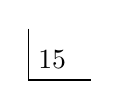
\begin{tikzpicture}[x=1cm,y=1cm,baseline=(pn.base)]
\node (pn) at (.3,.25) {$15$};
\draw[line width=.6pt] (0,.65)--(0,0)--(.8,0);
\end{tikzpicture}

\uwave{Одинаковые сист.} — отлич. либо числом частиц, либо сосудом.
(один. — масса и потенциал)

$\delta$ — содержится в $U(r)\,[?]$.


2. \uwave{Конфигурационная система}.

Получ. из предыдущ.
Состояние — $(x_1,\ldots,x_N)$ — область $\Omega^N$ либо её
подобласть $(\Omega_\delta)^N$.
\begin{equation*}
H(a)=\sum_{i\ne j}U(|x_i-x_j|)
\end{equation*}
— без кинетич. энергии.
\begin{equation*}
(\mathcal L_\sigma{}_{\Omega,N}\,[?],H^N_{U(r)})
\end{equation*}
\Unclear{GELFAND-P000152}{state-glyph}{Буква пространства состояний повторяет петлеобразный знак: $\mathcal L_\sigma$ / единая $\mathcal G$-подобная буква; правая петля может быть частью буквы или отдельным $\sigma$. Ниже $\Omega,N$.}
\end{GelfandAdjacentEvidence}

Система 1 сводится к системе 2. (см. ниже).


\par\noindent\begin{minipage}[t]{\linewidth}
3. \uwave{Модельная дискретная система}.

В $R^\nu$ кубич. решётка, $\Omega$ — её подмн-во.
Состояние — набор $N$ узлов решётки $(x_1,\ldots,x_N)$,
в котором нет двух равных.
\end{minipage}\par

$U(x)$ — чётная функция на решётке.
\begin{equation*}
H(a)=\sum_{i\ne j}U(x_i-x_j)
\end{equation*}
(Изотропность напр. — сферич. симм. — здесь не оправдана)


Результаты стат. физики зависят лишь от качеств.
свойств $U(r)\,[?]$, но физики используют лишь потенциал
\begin{equation*}
U(r)=\frac a{r^{12}}-\frac b{r^6},\qquad
\begin{gathered}a>0\mathstrut\\ b>0\end{gathered}
\end{equation*}
Нам важен рост в $0$ и убыв. на $\infty$.

\begin{GelfandAdjacentEvidence}{GELFAND-P000152}{2}
\SourceFigure{GELFAND-P000152}{potential-graph}{Вертикальная ось со стрелкой вверх; горизонтальная без установленной стрелки. Обе без букв. Ветвь идёт сверху справа от вертикальной оси, пересекает горизонталь, образует отрицательную впадину и приближается к горизонтали снизу. Верхний конец ветви густой, с короткими боковыми штрихами; его отдельное стрелочное значение не установлено. Точный масштаб не задан.\par\smallskip\centering{\color{black}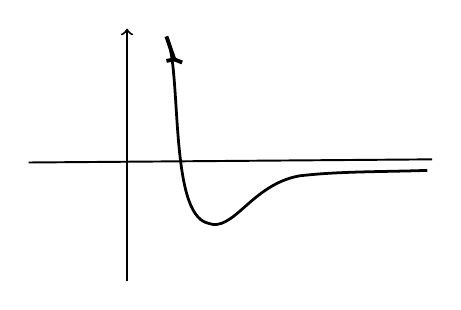
\begin{tikzpicture}[x=1.25cm,y=1cm]
\draw[->,line width=.7pt] (0,-1.5)--(0,1.7);
\draw[line width=.7pt] (-1,0)--(3.1,.04);
\draw[line width=1pt] (.4,1.6)..controls (.56,1.2) and (.42,-.65)..(.82,-.77)..controls (1.08,-.9) and (1.26,-.28)..(1.75,-.17)..controls (2.15,-.11) and (2.6,-.12)..(3.05,-.1);
\draw[line width=1.4pt] (.4,1.6)--(.48,1.31)--(.4,1.29);
\draw[line width=1.4pt] (.48,1.31)--(.56,1.27);
\end{tikzpicture}}}
\end{GelfandAdjacentEvidence}




\begin{GelfandAdjacentEvidence}{GELFAND-P000152}{3}
При наличии $\delta$:
\SourceFigure{GELFAND-P000152}{hard-core-graph}{Две оси со стрелками. Справа пунктирная вертикаль; над ней $+\infty$, у пересечения с горизонталью густой знак, справа $\delta$. Ветвь уходит от густого знака во впадину и поднимается ниже горизонтальной оси. Густота чернил в пересечении передана без установленного значения функции в $\delta$ или утверждения о замкнутости.\par\smallskip\centering{\color{black}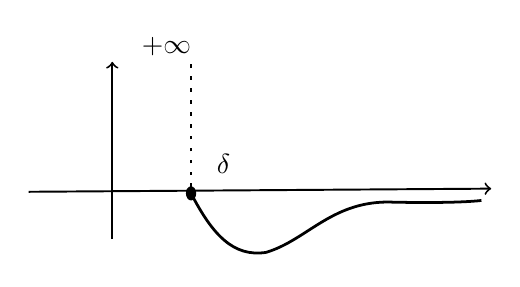
\begin{tikzpicture}[x=1.25cm,y=1cm]
\draw[->,line width=.7pt] (0,-.6)--(0,1.65);
\draw[->,line width=.7pt] (-.85,0)--(3.85,.04);
\draw[dash pattern=on 1.3pt off 3pt,line width=.8pt] (.8,.06)--(.8,1.65);
\node at (.55,1.85) {$+\infty$};
\node at (1.13,.35) {$\delta$};
\fill (.8,-.02) ellipse (.065cm and .09cm);
\draw[line width=1pt] (.8,-.02)..controls (1.02,-.55) and (1.23,-.83)..(1.56,-.77)..controls (1.97,-.62) and (2.22,-.13)..(2.8,-.13)..controls (3.12,-.14) and (3.55,-.14)..(3.75,-.11);
\end{tikzpicture}}}
\end{GelfandAdjacentEvidence}




\begin{GelfandAdjacentEvidence}{GELFAND-P000152}{4}
Иногда рассм. лишь финитный потенциал.
\Unclear{GELFAND-P000152}{potential-argument-glyph}{Повторяющаяся буква в $U(r)$ и знаменателях имеет петлеобразный верх с нижним штрихом вправо: $r$ / $\tau$-подобный знак. Передача как $r$ условна; исходные повторения видны во фрагментах.}
\end{GelfandAdjacentEvidence}




\begin{GelfandAdjacentEvidence}{GELFAND-P000153}{1}
\SourcePage{GELFAND-P000153}{unlabelled}
\uwave{Частицы малы ($\delta\,[?]$) по сравн. с областью.}
\Unclear{GELFAND-P000153}{top-smallness-glyph}{Знак в скобках: $\delta$- / $r$-подобный; верхняя часть касается верхней границы кадра и обрезана.}
\end{GelfandAdjacentEvidence}


Рассм. послед. сосудов $\Omega_N$, к-рая расширяется
и заполняет всё пр-во
(напр. подобные кубы)

\begin{GelfandAdjacentEvidence}{GELFAND-P000153}{2}
Рассмотрим
\begin{equation*}
\{\mathcal L_\sigma{}_{\Omega_N,N}\,[?],H^N_{m,U(r)}\}
\end{equation*}
\Unclear{GELFAND-P000153}{thermodynamic-state-glyph}{В первой фигурной скобке петлеобразная буква с правой петлёй: $\mathcal L_\sigma$ / единый $\mathcal G$-подобный знак; ниже $\Omega_N,N$. Передача основного знака условна.}
\end{GelfandAdjacentEvidence}

\begin{GelfandAdjacentEvidence}{GELFAND-P000153}{3}
\Unclear{GELFAND-P000153}{potential-argument-glyph}{Буква в $U(r)$ имеет короткий петлеобразный верх и нижний штрих вправо: $r$ / $\tau$-подобный знак. Передача как $r$ условна; исходная запись показана во фрагменте.}
\end{GelfandAdjacentEvidence}

\begin{equation*}
\frac{|\Omega_N|}{N}\longrightarrow v\quad\text{(предельный удельный объём)}
\end{equation*}
\begin{flushright}
$|\Omega_N|$ — объём области $\Omega_N$
\end{flushright}
(Термодинамич. пред. переход)

В большинстве случаев всё зависит только от $v$,
а форма сосуда несущественна.


\par\noindent\begin{minipage}[t]{\linewidth}
\uwave{Распределение Гиббса.}

\begin{GelfandAdjacentEvidence}{GELFAND-P000153}{4}
Считается, что на $\mathcal L_\sigma\,[?]$ задано распред. вероятностей
В равновесном случае оно постулируется
(если всё не зависит от времени)
\begin{equation*}
p(a)=\frac1Qe^{-\beta H(a)},\qquad\beta>0
\end{equation*}
\begin{equation*}
Q=\int_{\mathcal L_\sigma\,[?]}e^{-\beta H(a)}\,da.
\end{equation*}
\Unclear{GELFAND-P000153}{state-glyph}{Петлеобразная буква пространства состояний: $\mathcal L_\sigma$ / единый $\mathcal G$-подобный знак; правая петля может быть частью буквы или отдельным $\sigma$. Начертание повторено под интегралом.}
\end{GelfandAdjacentEvidence}
\end{minipage}\par



Для решётч. систем та же ф-ла, но $p$ — уже
сами вероятности, а не плотности.

Физич. сист. с зад. распред. Гиббса называется
\uwave{малым каноническим ансамблем}

\begin{GelfandAdjacentEvidence}{GELFAND-P000153}{5}
\begin{equation*}
\left(\begin{gathered}\text{в класс. случае}\\
\mathcal L_\sigma{}_{\Omega,N}\,[?],H^N_{m,U(r),\beta}\end{gathered}\right)
\end{equation*}
\Unclear{GELFAND-P000153}{ensemble-state-glyph}{В скобке о класс. случае снова петлеобразный знак пространства: $\mathcal L_\sigma$ / единая $\mathcal G$-подобная буква. Ниже $\Omega,N$; у $H$ сверху $N$, снизу $m,U(r),\beta$.}
\end{GelfandAdjacentEvidence}


При термодин. пред. перех. всегда рассм. одинаковые
системы ($\beta$ тоже фиксировано)
\begin{equation*}
p(a)=\frac1Qe^{-\beta\frac1{2m}\sum p_i^2}e^{-\beta\sum U(|x_i-x_j|)}
\end{equation*}

\begin{GelfandAdjacentEvidence}{GELFAND-P000153}{6}
\begin{equation*}
\mathcal L_\sigma\,[?]=R^{\nu N}\times\Omega^N
\end{equation*}
\Unclear{GELFAND-P000153}{product-state-glyph}{В последней строке тот же петлеобразный знак пространства; передача как $\mathcal L_\sigma$ условна. Справа $R^{\nu N}\times\Omega^N$.}
\end{GelfandAdjacentEvidence}



\begin{GelfandAdjacentEvidence}{GELFAND-P000154}{1}
\SourcePage{GELFAND-P000154}{16}
\hfill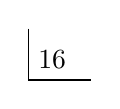
\begin{tikzpicture}[x=1cm,y=1cm,baseline=(pn.base)]
\node (pn) at (.3,.25) {$16$};
\draw[line width=.6pt] (0,.65)--(0,0)--(.8,0);
\end{tikzpicture}

Наше распред. есть произвед. более простых распределений
и интересно лишь распред. Гиббса в пр-ве конфигураций.
Там, где $U(r)\,[?]=+\infty$, плотность будет $0$.
Есть ф-и распред. для подсистемы ($\int$ по остальным)

\Unclear{GELFAND-P000154}{potential-argument-glyph}{Аргумент в $U(r)$: $r$ / $\tau$-подобный рукописный знак с короткой верхней петлёй и нижним изгибом. Передача как $r$ условна.}
\end{GelfandAdjacentEvidence}


Удобны \uwave{корреляционные функции}.
\begin{center}
\begin{tikzpicture}[x=1cm,y=1cm]
\node[anchor=north west,inner sep=0pt,text width=.58\linewidth,font=\small] (marginal) at (0,0) {
\begin{gather*}
p(x_1)=\frac1Q\int e^{-\beta\sum U(x_i-x_j)}\,dx_2\ldots dx_N\\
p(x_1,\ldots,x_k)=\ldots\int\ldots dx_{k+1}\ldots dx_N
\end{gather*}
};
\draw[line width=.6pt] ([xshift=-50mm,yshift=1mm]marginal.north west)--([xshift=-2mm,yshift=1mm]marginal.north west);
\draw[line width=.6pt] ([xshift=-2mm,yshift=1mm]marginal.north west)--([xshift=-2mm,yshift=-1mm]marginal.south west);
\draw[line width=.6pt] ([xshift=-3.5mm]marginal.north west)--([xshift=-3.5mm,yshift=-1mm]marginal.south west);
\draw[line width=.6pt] ([xshift=-3.5mm]marginal.south west)--(marginal.south east);
\end{tikzpicture}
\end{center}

\begin{GelfandAdjacentEvidence}{GELFAND-P000154}{2}

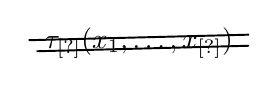
\begin{tikzpicture}[baseline=(cancelled.base)]
\node[inner sep=0pt] (cancelled) {$\tau_{[?]}(x_1,\ldots,x_{[?]})$};
\draw[line width=.7pt] ([xshift=-2mm,yshift=1pt]cancelled.west)--([xshift=2mm,yshift=3pt]cancelled.east);
\draw[line width=.7pt] ([xshift=-1mm,yshift=-3pt]cancelled.west)--([xshift=2mm,yshift=-1pt]cancelled.east);
\end{tikzpicture}
\Unclear{GELFAND-P000154}{cancelled-correlation}{Зачёркнуто выражение, похожее на $\tau_k(x_1,\ldots,x_N)$ / $\tau_2(x_1,\ldots,x_2)$; нижние индексы и средние штрихи перекрыты двумя линиями. Первоначальные индексы не установлены.}
\end{GelfandAdjacentEvidence}
\begin{GelfandAdjacentEvidence}{GELFAND-P000154}{3}

\begin{equation*}
\tau_k(x_1,\ldots,x_k\mid N,\Omega,\beta)\,[?]=\frac{N!}{(N-k)!}p(x_1,\ldots,x_k)
\end{equation*}
\Unclear{GELFAND-P000154}{correlation-glyph}{Корреляционный знак с короткой верхней волной и нисходящим изгибом: $\tau$ / $r$-подобный. Здесь и в повторениях $\tau$ — условная передача.}
\end{GelfandAdjacentEvidence}


\uwave{Сумматорная ф-я} $F(a)$, $a\,(x_1,\ldots,x_N)$

1-го порядка $F(a)=f(x_1)+f(x_2)+\ldots+f(x_N)$

2-го порядка $F(a)=\sum_{i\ne j}f(x_i,x_j)$, $f$ — симметрич.

и так далее.

\begin{GelfandAdjacentEvidence}{GELFAND-P000154}{4}

\uwave{Среднее для сумматорных ф-й $F$}:
\begin{align*}
\langle F\rangle&=N\langle f(x_1)\rangle=N\int_\Omega f(x)p(x)\,dx\\
&=\int_\Omega f(x)\tau_1(x)\,[?]\,dx
\end{align*}
(достат. знать 1-ю корреляц. функцию)
\Unclear{GELFAND-P000154}{first-moment}{В первой формуле среднего знак перед индексом $1$ повторяет $\tau$ / $r$-подобное начертание; $\tau_1$ — условная передача. Обе области интегрирования явно $\Omega$.}
\end{GelfandAdjacentEvidence}


\begin{GelfandAdjacentEvidence}{GELFAND-P000154}{5}
Аналогично для 2-го порядка:
\begin{equation*}
\langle F\rangle=\iint_{\Omega\,\Omega}f(x_1,x_2)\tau_2(x_1,x_2)\,[?]\,dx_1dx_2
\end{equation*}
\Unclear{GELFAND-P000154}{second-moment}{Во второй формуле среднего тот же $\tau$ / $r$-подобный знак, здесь с индексом $2$. Под двойным интегралом написаны два $\Omega$.}
\end{GelfandAdjacentEvidence}


\uwave{Вероятностный (физич.) смысл.}

$C\subset\Omega$, $C$ — подобласть, $n_C(a)$ — число частиц,
попавших в подобласть, $a=(x_1,\ldots,x_N)$.
Это сумматорная велич. 1-го порядка, причём
\begin{equation*}
f(x)=\begin{cases}1,&x\in C,\\0,&x\notin C\end{cases}
\end{equation*}

\begin{GelfandAdjacentEvidence}{GELFAND-P000154}{6}
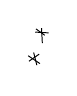
\begin{tikzpicture}[x=1mm,y=1mm,baseline=0pt]
\draw[line width=.35pt] (1,3.2)--(.9,5.1);
\draw[line width=.35pt] (.1,4.6)--(1.8,4.5);
\draw[line width=.35pt] (.2,5)--(1.3,4.2);
\draw[line width=.35pt] (-.8,1.6)--(.7,.6);
\draw[line width=.35pt] (-.7,.9)--(.6,1.8);
\draw[line width=.35pt] (-.1,2)--(.3,.4);
\end{tikzpicture}
\Unclear{GELFAND-P000154}{left-margin-marks}{В левом поле два мелких угловатых перекрещённых знака; их буквенное чтение и значение не установлены.}
\end{GelfandAdjacentEvidence}


\begin{GelfandAdjacentEvidence}{GELFAND-P000154}{7}
Поэтому
\begin{equation*}
\langle n_C(a)\rangle=\int_C\tau_1(x)\,[?]\,dx
\end{equation*}
\begin{equation*}
\frac{\langle n_C(a)\rangle}{|C|}=\frac1{|C|}\int\tau_1(x)\,[?]\,dx
\end{equation*}
\Unclear{GELFAND-P000154}{last-integral-domain}{У последнего интеграла нижний предел не виден; в предшествующей формуле явно $C$. Повторяющийся корреляционный знак передан условно как $\tau_1$.}
\end{GelfandAdjacentEvidence}



\begin{GelfandAdjacentEvidence}{GELFAND-P000155}{1}
\SourcePage{GELFAND-P000155}{unlabelled}
Для малой области получим, что
$\tau_1(x)\,[?]$ — „локальная средняя плотность“
в точке $x$.
\Unclear{GELFAND-P000155}{local-density-glyph}{В начале знак перед индексом $1$: $\tau$ / $r$-подобный рукописный знак; передача как $\tau_1$ условна.}
\end{GelfandAdjacentEvidence}


\begin{GelfandAdjacentEvidence}{GELFAND-P000155}{2}
\uwave{Ещё вероятн. смысл}:
\SourceFigure{GELFAND-P000155}{small-neighbourhood}{Отдельный приблизительный кружок с точкой внутри; у верхнего правого края $\Delta C$, снизу $x_0$.\par\smallskip\centering{\color{black}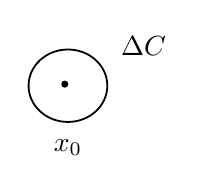
\begin{tikzpicture}[x=1cm,y=1cm]
\draw[line width=.65pt] (0,0) ellipse (.5cm and .46cm);
\fill (-.04,.02) circle (.045cm);
\node at (.96,.5) {$\Delta C$};
\node at (0,-.78) {$x_0$};
\end{tikzpicture}}}
\end{GelfandAdjacentEvidence}


$\Delta C$ — малая окр. $x_0$.

\begin{GelfandAdjacentEvidence}{GELFAND-P000155}{3}
Вероятность того, что $n_{\Delta C}=1$
есть $\tau_1(x_0)\,[?]\Delta C$.
\begin{equation*}
p(n_{\Delta C}=1)=\tau_1(x_0)\,[?]\Delta C+o(\Delta C)
\end{equation*}
\Unclear{GELFAND-P000155}{probability-expansion}{В словесной строке и в равенстве повторён условно переданный знак $\tau_1$. Последний член записан $o(\Delta C)$.}
\end{GelfandAdjacentEvidence}
\begin{GelfandAdjacentEvidence}{GELFAND-P000155}{4}


\begin{tikzpicture}[x=1cm,y=1cm,baseline=0pt]
\fill (0,0)--(-.07,.05)--(-.08,.15)--(-.03,.12)--(.02,.15)--(.06,.13)--(.1,.18)--(.15,.16)--(.15,.07)--(.1,.03)--(.06,-.02)--cycle;
\end{tikzpicture}
\Unclear{GELFAND-P000155}{isolated-ink-mark}{Между строками первого вероятностного пояснения отдельное густое пятно с неровным контуром; буквенное чтение и значение не установлены.}
\end{GelfandAdjacentEvidence}


26/$\overline{\underline{\mathrm{IX}}}$. \uwave{Сем. Гельфанда}.

\uwave{Р.А. Минлос}. \underline{Лекция 2}.

$\tau(x_1,x_2)\,[?]\Delta x_1\Delta x_2$ — вероятн. попад.
$\overset{\underbrace{\text{(одной)}}}{\text{частицы}}$ в $\Delta x_1$
и второй в $\Delta x_2$.

\begin{GelfandAdjacentEvidence}{GELFAND-P000155}{5}
\Unclear{GELFAND-P000155}{two-particle-correlation-glyph}{Перед $(x_1,x_2)$ тот же $\tau$ / $r$-подобный знак; отдельный индекс $2$ у него не виден. Передача как $\tau$ условна.}
\end{GelfandAdjacentEvidence}

\begin{GelfandAdjacentEvidence}{GELFAND-P000155}{6}
\SourceFigure{GELFAND-P000155}{two-neighbourhoods}{Два отдельных приблизительных контура, снизу $x_1,x_2$; внутри густые перекрещённые штрихи, их отдельное буквенное чтение не установлено. Над правым контуром короткий штрих. Размеры и расстояние не заданы.\par\smallskip\centering{\color{black}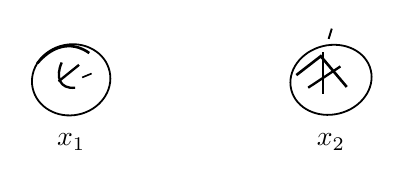
\begin{tikzpicture}[x=1cm,y=1cm]
\draw[line width=.65pt,rotate=12] (0,0) ellipse (.5cm and .45cm);
\draw[line width=.95pt] (-.43,.21)..controls (-.2,.48) and (.05,.47)..(.23,.34);
\draw[line width=.85pt] (-.12,.22)..controls (-.2,.04) and (-.15,-.12)..(.05,-.1);
\draw[line width=.85pt] (-.16,-.02)--(.1,.19);
\draw[line width=.6pt] (.14,.03)--(.26,.08);
\node at (0,-.79) {$x_1$};
\draw[line width=.65pt,rotate around={14:(3.3,0)}] (3.3,0) ellipse (.52cm and .44cm);
\draw[line width=.95pt] (2.86,.06)--(3.17,.3)--(3.5,-.09);
\draw[line width=.85pt] (3.2,.35)--(3.2,-.18);
\draw[line width=.85pt] (3.01,-.1)--(3.42,.17);
\draw[line width=.7pt] (3.27,.52)--(3.31,.65);
\node at (3.3,-.79) {$x_2$};
\end{tikzpicture}}}
\end{GelfandAdjacentEvidence}




$\Omega_N\longrightarrow\infty$ — термодин. пред. переход.
\begin{equation*}
\frac{|\Omega_N|}{N}\longrightarrow v=\frac1\rho,\qquad\rho\text{ — плотность}.
\end{equation*}


\underline{Гипотеза}: 1)
\begin{equation*}
\tau_k(x_1,\ldots,x_k\mid N,\Omega,\beta)\,[?]\longrightarrow\vec\tau_k(x_1,\ldots,x_k\mid v,\beta)\,[?]
\end{equation*}
Это предполагается (предельная корреляц. функция)

\begin{GelfandAdjacentEvidence}{GELFAND-P000155}{7}
Более того, предполагается, что $\forall\tau_k\ \exists v_N$, такое что
\begin{equation*}
\bigl(v_N\ \underset{\longrightarrow}{\text{зависит}}\text{ лишь от сосуда и от}\,[?]\ k\bigr)
\end{equation*}
\Unclear{GELFAND-P000155}{volume-parenthesis}{Короткая запись перед $k$: «от» / «о.»-подобное сокращение; чтение не установлено. Под словом «зависит» отдельная стрелка вправо.}
\end{GelfandAdjacentEvidence}
\begin{GelfandAdjacentEvidence}{GELFAND-P000155}{8}

\begin{align*}
2)\quad &\left|\begin{aligned}
\tau_k(x_1,\ldots,x_k\mid N,\Omega,\beta)\,[?]\\[-.3ex]
-\vec\tau_k(x_1,\ldots,x_k\mid v_N,\beta)\,[?]
\end{aligned}\right|<\\
&<C_k\gamma\bigl(\min\underset{\text{расст.}}{|x_i,\partial\Omega|}\bigr),\\
&\text{где }\gamma(r)\longrightarrow0\text{ при }r\longrightarrow\infty.
\end{align*}
\Unclear{GELFAND-P000155}{correlation-glyph}{Основная буква: $\tau$ / $r$-подобный знак. Над предельной функцией горизонтальный штрих с наконечником вправо. В оценке $\gamma$ с длинным нижним ходом; под $|x_i,\partial\Omega|$ приписано «расст.».}
\end{GelfandAdjacentEvidence}
\begin{GelfandAdjacentEvidence}{GELFAND-P000155}{9}

\begin{flushright}
\begin{tikzpicture}[x=1cm,y=1cm]
\node[anchor=north west,inner sep=0pt,text width=.32\linewidth] (margin) at (0,0) {Объём\,[?]\par и $v$\,[?]\par обсуждаем\,[?]\par Идеальный\par газ — всё\,[?]\par [густой неразобранный знак]\par $\operatorname{const}$ и\par надо получ. $0$};
\draw[line width=.65pt] ([xshift=-2mm]margin.north west)--([xshift=-2mm]margin.south west);
\draw[line width=.65pt] ([xshift=-3.5mm]margin.north west)--([xshift=-3.5mm]margin.south west);
\end{tikzpicture}
\end{flushright}
\Unclear{GELFAND-P000155}{right-margin}{За двумя вертикальными чертами слова, похожие на «Объём и $v$ обсуждаем», затем «Идеальный газ — всё» / «… без …», $\operatorname{const}$, «и надо получ. $0$». Первая связка и окончания бледны; после строки о газе густой неразобранный знак. Приведённые чтения условны.}
\end{GelfandAdjacentEvidence}


\begin{GelfandAdjacentEvidence}{GELFAND-P000155}{10}
$\gamma$ зависит от потенциала.
Для финитного потенциала $\gamma(r)\longrightarrow e^{-\lambda r}$.
\Unclear{GELFAND-P000155}{exponential-arrow}{Между $\gamma(r)$ и $e^{-\lambda r}$ стрелка вправо; отдельные условия предела в этой строке не повторены.}
\end{GelfandAdjacentEvidence}
\begin{GelfandAdjacentEvidence}{GELFAND-P000155}{11}

\sout{[неразобранный знак]}
\Unclear{GELFAND-P000155}{cancelled-before-volume}{Перед «Имеем» густо зачёркнут короткий знак или номер; первоначальное чтение не установлено.}
\end{GelfandAdjacentEvidence}

Имеем тогда $v_N\longrightarrow v$ при $N\longrightarrow\infty$.

\begin{GelfandAdjacentEvidence}{GELFAND-P000155}{12}
3) Предполож., что пред. корреляц. ф-и инвар. отн. сдвигов.
Отсюда $\vec\tau_1\,[?]=\operatorname{const}=\rho$.
\Unclear{GELFAND-P000155}{final-invariance-glyph}{В последней строке повторён условно переданный знак $\tau_1$ с горизонтальной стрелкой вправо над ним; далее $\operatorname{const}=\rho$.}
\end{GelfandAdjacentEvidence}



\begin{GelfandAdjacentEvidence}{GELFAND-P000156}{1}
\SourcePage{GELFAND-P000156}{17}
\hfill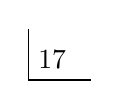
\begin{tikzpicture}[x=1cm,y=1cm,baseline=(pn.base)]
\node (pn) at (.3,.25) {$17$};
\draw[line width=.6pt] (0,.65)--(0,0)--(.8,0);
\end{tikzpicture}

4) Непрерывность относительно $v$ и $\beta$.

Эта теорема должна быть верна кроме исключит.
значений $v$ и $\beta$. (предполагается)

Доказана лишь для малых $v$ и $\beta$ (при нек-рых предполож.).
(это будет сделано в дальнейшем —
— Ruelle)


5) Все $\vec\tau_k\,[?]$ ограничены.
\hfill
\begin{tikzpicture}[x=1cm,y=1cm,baseline=0pt]
\fill (0,.04)--(.16,.07)--(.16,-.05)--(.08,-.02)--(.02,-.04)--cycle;
\end{tikzpicture}
\Unclear{GELFAND-P000156}{limiting-correlation-glyph}{Основная буква $\tau$ / $r$-подобна; передача как $\tau$ условна. Над ней горизонтальный штрих с наконечником вправо; в обеих строках пункта $5$ индекс $k$.}
\end{GelfandAdjacentEvidence}
\begin{GelfandAdjacentEvidence}{GELFAND-P000156}{2}

$\vec\tau_k\,[?]$ существ. при всех $v$, не\,[?] при всех $v$ такая\,[?]
скорость сходимости.
\Unclear{GELFAND-P000156}{fifth-hypothesis-correction}{Короткое слово после запятой: «не» / «но». Начало слова, переданного как «такая», густо переправлено; первоначальное чтение под штрихами не установлено.}
\end{GelfandAdjacentEvidence}
\begin{GelfandAdjacentEvidence}{GELFAND-P000156}{3}

\begin{center}
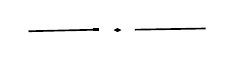
\begin{tikzpicture}[x=1cm,y=1cm]
\draw[line width=.6pt] (0,0)--(.87,.02);
\draw[line width=1.2pt] (.82,.02)--(.9,.02);
\fill (1.08,.015)--(1.13,.04)--(1.18,.015)--(1.13,-.01)--cycle;
\draw[line width=.6pt] (1.35,.02)--(2.25,.035);
\end{tikzpicture}
\end{center}
\Unclear{GELFAND-P000156}{separators-and-ink}{Справа возле пункта $5$ отдельный небольшой густой знак с неровным контуром; буквенное чтение не установлено. Ниже две горизонтальные черты и отдельная средняя точка ромбовидной формы; правый конец левой черты утолщён.}
\end{GelfandAdjacentEvidence}


\begin{GelfandAdjacentEvidence}{GELFAND-P000156}{4}
\uwave{О распределении Гиббса.} (по просьбе Гельфанда)
\begin{equation*}
a(p_1,\ldots,p_N,x_1,\ldots,x_N)
\end{equation*}
\SourceFigure{GELFAND-P000156}{energy-circle}{Один незаполненный приблизительный круг без подписей и стрелок слева от абзаца о движении; размеры не заданы.\par\smallskip\centering{\color{black}\begin{tikzpicture}[x=1cm,y=1cm]
\draw[line width=.65pt,rotate=-4] (0,0) ellipse (.62cm and .55cm);
\end{tikzpicture}}}
\end{GelfandAdjacentEvidence}



Движ. по поверхн. пост. энергии $H(a)=\operatorname{const}$.
Предполож., что она эргодична и есть инвар. мера.

Может быть, любое распред. при увелич. числа частиц
приводит к распр. Гиббса. (Гельфанд)

Не любое: если нет эргодич. гипотезы (Арнольд)
\begin{center}
\begin{tikzpicture}[x=1cm,y=1cm]
\draw[line width=.6pt] (0,0)--(.9,.04);
\draw[line width=1.15pt] (.83,.035)--(.91,.04);
\fill (1.09,.02) circle (.035cm);
\draw[line width=.6pt] (1.3,.025)--(2.28,.09);
\end{tikzpicture}
\end{center}


\uwave{Репрезентативность средних значений.}
\begin{equation*}
P_\sigma\,[?]\bigl(|F-\langle F\rangle|>\varepsilon\bigr)\longrightarrow0
\quad\text{при увелич. числа частиц.}
\end{equation*}
Тогда случ. велич. (ф-я; физич. величина) называется
репрезентативной.

\begin{GelfandAdjacentEvidence}{GELFAND-P000156}{5}
Это неточно, т.к. нет единой ф-и $F$.
\Unclear{GELFAND-P000156}{probability-subscript}{Индекс у $P$ короткий, с верхним загибом и нижней петлёй: $\sigma$ / $\tau$ / $r$-подобный знак. Передача как $\sigma$ условна. Заголовок волнисто подчёркнут; ниже замечание об отсутствии единой функции $F$.}
\end{GelfandAdjacentEvidence}


\uwave{Нужный пример.} (сумматорная функция)
\begin{equation*}
F_N(x_1,\ldots,x_N)=\sum_{i\ne j}f(x_i-x_j),
\end{equation*}
$f$ одна и та же, $\displaystyle\int|f(\xi)|\,d\xi<\infty$.

\begin{GelfandAdjacentEvidence}{GELFAND-P000156}{6}
\begin{align*}
\langle F_N\rangle
&=\iint\tau_2\,[?](x_1,x_2\mid N,\Omega,\beta)f(x_1-x_2)\,dx_1\,dx_2=\\
&=\iint\vec\tau_2\,[?](x_1-x_2\mid v,\beta)f(x_1-x_2)\,dx_1\,dx_2+o(|\Omega|)=\\
&=|\Omega|\int\vec\tau_2\,[?](\xi\mid v,\beta)f(\xi)\,d\xi+o(|\Omega|).
\end{align*}
\Unclear{GELFAND-P000156}{mean-correlation-glyph}{В первой строке основной $\tau$ / $r$-подобный знак без верхнего штриха, в следующих двух над ним штрих с наконечником вправо; в трёх строках индекс $2$. Буква передана условно. Области интегрирования отдельно не подписаны; знаки равенства повторены на концах и началах строк.}
\end{GelfandAdjacentEvidence}
\begin{GelfandAdjacentEvidence}{GELFAND-P000156}{7}

\begin{flushright}
\begin{tikzpicture}[x=1cm,y=1cm,baseline=0pt]
\draw[line width=.7pt] (0,.02)..controls (-.18,.1) and (-.05,.25)..(.1,.18)..controls (.22,.12) and (.06,-.09)..(-.09,-.04);
\draw[line width=.55pt] (-.14,-.06)--(.58,.22);
\draw[line width=.55pt] (-.1,-.1)--(.62,.18);
\node at (1,.27) {$+$};
\node at (2.55,.27) {$F\,[?]$};
\draw[line width=.6pt] (1.55,-.08)--(2.91,.63);
\draw[line width=.6pt] (1.6,-.16)--(2.98,.57);
\draw[line width=.45pt] (1.62,-.22)--(2.85,.48);
\end{tikzpicture}
\end{flushright}
\Unclear{GELFAND-P000156}{cancelled-final-equation}{Справа от последнего равенства перечёркнуты петлеобразный знак, плюс и $F$-подобное начертание. Первое чтение не установлено; $F$ условно. Зачёркивающие штрихи наклонные.}
\end{GelfandAdjacentEvidence}


\begin{GelfandAdjacentEvidence}{GELFAND-P000156}{8}
Итак,
\begin{equation*}
\left\langle\frac{F_N}{N}\right\rangle\sim v\int\vec\tau_k\,[?](\xi\mid v,\beta)f(\xi)\,d\xi
\quad\text{— уже }\operatorname{const}.
\end{equation*}
\Unclear{GELFAND-P000156}{final-index}{Последний индекс $k$- / $2$-подобен; передан как $k$ условно. Над основной буквой горизонтальный штрих с наконечником вправо; сама буква $\tau$ / $r$-подобна. Перед интегралом написано $v$.}
\end{GelfandAdjacentEvidence}



\begin{GelfandAdjacentEvidence}{GELFAND-P000157}{1}
\SourcePage{GELFAND-P000157}{unlabelled}
\begin{tikzpicture}[x=1cm,y=1cm,baseline=(cancel.base)]
\node (cancel) at (0,0) {$6\,[?]$};
\draw[line width=1.15pt] (-.22,-.02)--(.22,.06);
\draw[line width=.9pt] (-.2,.04)--(.2,.12);
\fill (.35,.02) circle (.035cm);
\end{tikzpicture}
\Unclear{GELFAND-P000157}{cancelled-top-number}{В верхнем левом поле густо зачёркнутый петлеобразный знак, похожий на $6$; первоначальное чтение не установлено. Справа отдельная точка.}
\end{GelfandAdjacentEvidence}
\begin{GelfandAdjacentEvidence}{GELFAND-P000157}{2}

Ещё одна гипотеза (но она уже выводится из этих,
хотя и сложно):
\begin{align*}
6)\quad&\left|\begin{aligned}
\bar\tau_{k+s}(x_1,\ldots,x_k,y_1,\ldots,y_s\mid v,\beta)\\[-.3ex]
-\bar\tau_k(x_1,\ldots,x_k\mid v,\beta)\bar\tau_s(y_1,\ldots,y_s\mid v,\beta)
\end{aligned}\right|\,[?]\le\\
&\le C_{k,s}\gamma\bigl(\min_{i,j}|x_i-y_j|\bigr)\,[?].
\end{align*}
(мультиплик. свойство; для идеального газа $0$).
\Unclear{GELFAND-P000157}{hypothesis-correlation-glyph}{Основная буква во всех трёх функциях $\tau$ / $r$-подобна; передача как $\tau$ условна. Над каждой плоский горизонтальный штрих. У минимума $i,j$; между $x_i$ и $y_j$ густой горизонтальный знак, переданный как минус. Знаки $\le$ повторены на конце и начале строк.}
\end{GelfandAdjacentEvidence}


Докажем, что
\begin{equation*}
\underset{\text{дисперсия}}{DF_N}\sim dN,\qquad d\text{ — }\operatorname{const}.
\end{equation*}
Отсюда $D\frac{F_N}{N}\sim\frac dN$ и по нер-ву Чебышева уже

\begin{GelfandAdjacentEvidence}{GELFAND-P000157}{3}
получается
\begin{tikzpicture}[x=1cm,y=1cm,baseline=(word.base)]
\node[inner sep=1pt] (word) at (0,0) {[неразобранное слово]};
\draw[line width=.9pt] (word.west)--(word.east);
\draw[line width=.8pt] ([yshift=-1mm]word.west)--([yshift=1mm]word.east);
\draw[line width=.6pt] (-.65,-.05)..controls (-.95,-.5) and (-.65,-.5)..(-.48,-.18);
\end{tikzpicture}
репрезент. среднего.
\Unclear{GELFAND-P000157}{cancelled-representative-word}{После «получается» густо зачёркнуто слово с нижним петлеобразным штрихом. Первоначальное чтение, в том числе возможное повторение «репрезент.», не установлено. Далее написано «репрезент. среднего».}
\end{GelfandAdjacentEvidence}

Это док. непосредств. подсчётом:
\begin{equation*}
DF_N=\langle F_N^2\rangle-\langle F_N\rangle^2.
\end{equation*}

\begin{GelfandAdjacentEvidence}{GELFAND-P000157}{4}
\begin{align*}
\begin{tikzpicture}[x=1cm,y=1cm,baseline=(square.base)]
\node (square) at (0,0) {$F_N^2$};
\node[anchor=north east,align=left,inner sep=1pt] (ann) at (.25,-.56) {$\substack{\text{суммат.}\,[?]\\\text{велич. 4-го пор.}}$};
\draw[line width=.65pt] (-.42,-.18)..controls (-.28,-.45) and (.28,-.45)..(.42,-.18);
\draw[line width=.55pt] ([xshift=-1mm,yshift=-2mm]ann.south west)..controls ([yshift=-2mm]ann.south) and ([xshift=3mm,yshift=-2mm]ann.south east)..([xshift=4mm,yshift=-1mm]ann.south east)..controls ([xshift=6mm]ann.east) and ([xshift=5mm,yshift=-1mm]ann.north east)..([xshift=3mm,yshift=-1mm]ann.north east);
\end{tikzpicture}
&=2\sum_{i\ne j}f^2(x_i-x_j)\\
&\quad+4\sum_{\substack{i,j,k\,[?]\\\text{несовп.}\,[?]}}f(x_i-x_j)f(x_k-x_j)+\\
&\quad+\sum_{\substack{i,j,k,s\\\text{неравны}}}f(x_i-x_j)f(x_k-x_s).
\end{align*}
\Unclear{GELFAND-P000157}{sum-labels}{Под $F_N^2$ короткая дуга; слева приписано «суммат.» / сходное сокращение, затем «велич. 4-го пор.», охваченные снизу длинной изогнутой чертой. Под тройной суммой $i,j,k$-подобный густой третий знак и «несовп.»-подобное сокращение; эти чтения условны. Под четвёрной — $i,j,k,s$ и «неравны».}
\end{GelfandAdjacentEvidence}


\begin{GelfandAdjacentEvidence}{GELFAND-P000157}{5}

Вычисляем
\begin{equation*}
\langle F_N^2\rangle=2\iint f^2(x_1-x_2)\tau_2\,[?](x_1,x_2)\,dx_1\,dx_2+4\ldots
\end{equation*}
и пользуемся оценками убывания.
\Unclear{GELFAND-P000157}{terminal-correlation-glyph}{У функции в последнем интеграле основной $\tau$ / $r$-подобный знак без верхнего штриха и индекс $2$; передача буквы как $\tau$ условна. Далее $+4\ldots$ и полная строка об оценках убывания.}
\end{GelfandAdjacentEvidence}



\begin{GelfandAdjacentEvidence}{GELFAND-P000158}{1}
\SourcePage{GELFAND-P000158}{18}
\hfill\begin{tikzpicture}[x=1cm,y=1cm,baseline=(pn.base)]
\node (pn) at (.3,.25) {$18$};
\draw[line width=.6pt] (0,.65)--(0,0)--(.8,0);
\end{tikzpicture}

\underline{Д. Каждан.} \uwave{Его результаты.}

1) $G$ — простая, вещ. или $p$-адич. группа Ли, содержащая
в кач. подгр. $SL(3,P)\,[?]$, $P\,[?]$ — соотв. поле.
$\Gamma$ — дискр. подгруппа с конечным объёмом факторпр-ва.
\Unclear{GELFAND-P000158}{field-and-group-glyphs}{В аргументе $SL(3,P)$ и перед словами «соотв. поле» знак с верхней петлёй и нижним ходом: $P$ / $\rho$-подобное начертание. Передача как $P$ условна.}
\end{GelfandAdjacentEvidence}

Тогда а)
\begin{equation*}
\Gamma/\underset{\substack{\vert\\\text{коммутант}}}{[\Gamma,\Gamma]}\quad\text{конечна}.
\end{equation*}
б) $\Gamma$ имеет конечное число образующих.
(даже из любого набора образ. выд. конечное)


2) $G$ — алгебр. группа над рац. числами $Q$, содерж.
$SL(3,Q)$.
Что-то о представлениях.

\uwave{Док-во} использует изолированность единичного представления.

\begin{GelfandAdjacentEvidence}{GELFAND-P000158}{2}

\underline{\uwave{Проф. Лоджс.\,[?] (Канада)}} совм. с \uwave{P. Szego}.
\Unclear{GELFAND-P000158}{lecturer-name}{Имя: «Лоджс.» / «Ходжс.» / «Лорчс.» / «Лорче.»; первая буква густая, в середине заметная верхняя петля, в конце $c$-подобный знак. Чтение условно. Под строкой о профессоре и Канаде волнистая и прямая линии; под P. Szego — волнистая.}
\end{GelfandAdjacentEvidence}
\begin{GelfandAdjacentEvidence}{GELFAND-P000158}{3}

\begin{equation*}
y''+f(x)y=0,\qquad0<x<\infty.
\end{equation*}
\SourceFigure{GELFAND-P000158}{oscillating-solution}{Горизонтальная линия, короткая вертикаль слева, четыре густых первых пересечения и точка внизу вертикали. Три верхние волны чередуются с нижними, справа короткий загнутый вниз конец. Подписей, размеров и точных координат нет; контур приблизителен.\par\smallskip\centering{\color{black}\begin{tikzpicture}[x=1cm,y=1cm]
\draw[line width=.65pt] (-.85,-.02)--(4.35,.02);
\draw[line width=.65pt] (0,.72)--(0,-.58);
\draw[line width=.85pt] (0,0)..controls (.13,.6) and (.5,.65)..(.82,.62)..controls (1.02,.61) and (1.08,.27)..(1.18,0)..controls (1.32,-.58) and (1.73,-.7)..(2.04,0)..controls (2.2,.4) and (2.48,.58)..(2.65,0)..controls (2.78,-.44) and (3.01,-.48)..(3.13,0)..controls (3.25,.31) and (3.5,.43)..(3.47,0)..controls (3.53,-.18) and (3.65,-.17)..(3.74,-.13);
\fill (0,0) circle (.065cm);
\fill (1.18,0) circle (.065cm);
\fill (2.04,0) circle (.065cm);
\fill (2.65,0) circle (.065cm);
\fill (0,-.58) circle (.035cm);
\end{tikzpicture}}}
\end{GelfandAdjacentEvidence}




\uwave{Штурм:} (1836)
если $f(x)$ возраст., то нули сближаются
и наоборот.

\par\noindent\begin{minipage}[t]{\linewidth}
\uwave{Теорема,} если $f$ облад. более высокой степ. монотонности.

Пусть
\begin{equation*}
(-1)^j f^{(j+1)}(x)\ge0,\qquad0<x<\infty,\quad j=1,\ldots,N
\end{equation*}
\end{minipage}\par
и $f(\infty)>0$. Тогда
\begin{equation*}
(-1)^n\Delta^{n+1}x_k>0,\qquad n=1,\ldots,N+1;\quad k=1,2,\ldots
\end{equation*}

\begin{GelfandAdjacentEvidence}{GELFAND-P000158}{4}
Это вып. для ф-й Bessel
\raisebox{.65ex}{\begin{tikzpicture}[baseline=(order.base)]
\node[draw,ellipse,inner sep=2pt,line width=.6pt] (order) {$\nu>\frac12\,[?]$};
\end{tikzpicture}}, \textbf{A}iry\,[?] и др.
\Unclear{GELFAND-P000158}{bessel-insertion}{В овальном контуре над строкой после Bessel: $\nu>1/2$ / $v>1/2$; знак и густая дробь переданы условно. Следующее имя Airy / Аiry: начальный $A$-подобный знак густо переправлен, затем точка над $i$, $r$-подобное соединение и нижняя петля $y$.}
\end{GelfandAdjacentEvidence}


Площади волн обладают тем же свойством.
\begin{equation*}
M_k=\int_{x_k}^{x_{k+1}}|y(x)|^\lambda\,dx,\qquad\lambda>-1.
\end{equation*}
$\lambda=0$ — разности нулей, $\lambda=1$ — площади волн,

\begin{GelfandAdjacentEvidence}{GELFAND-P000158}{5}
$\lambda=-1$ —
$\underset{\text{([неразобранное сокращение] части)}}{\text{разн. произв.}}$
(замеч. Гельфанда) $\dfrac1{y'(x_k)}$.
\Unclear{GELFAND-P000158}{last-parenthesis}{Под «разн. произв.» скобка: «ин. части» / «м. части» / «… части»; первое сокращение не установлено. В основной строке $\lambda=-1$; справа $1/y'(x_k)$.}
\end{GelfandAdjacentEvidence}



\begin{GelfandAdjacentEvidence}{GELFAND-P000159}{1}
\SourcePage{GELFAND-P000159}{unlabelled}
\underline{\underline{И.М. Гельфанд.}}

Повторение И. Бернштейна. (он же Atiya)

$G$ — компактная группа.
$K_G$ — функтор, $K_G(X)$.

\SourceFigure{GELFAND-P000159}{bundle-map}{$E$ над $X$, между ними стрелка вниз, без дополнительных подписей.\par\smallskip\centering{\color{black}\begin{tikzpicture}[x=1cm,y=1cm]
\node at (0,.7) {$E$};
\draw[->,line width=.7pt] (0,.4)--(0,-.4);
\node at (0,-.7) {$X$};
\end{tikzpicture}}}
\end{GelfandAdjacentEvidence}



$E,X$ — $G$-пр-ва; вект. расслоение.
Слой в слой — линейно.
Формальные разности.

Это контравариантный функтор.


\uwave{Обобщение понятия классифицир. пр-ва.}
Рассм.
\begin{equation*}
E\times_G X=X_G.
\end{equation*}
траект. $G$ стяг. в точку; $E$ — универс. пр-во.

\begin{GelfandAdjacentEvidence}{GELFAND-P000159}{2}
Если $\boldsymbol X$ — точка, то $X_G=B_G$, т.е. $*_G=B_G$.
\Unclear{GELFAND-P000159}{cancelled-point-x}{После «Если» густой $X$ поверх прежних штрихов. Первоначальное чтение под ними не установлено.}
\end{GelfandAdjacentEvidence}


\underline{Теорема.} $K_G(X)$ приблизительно совпад. с $K(X_G)$
(уже обычный $K$-функтор)

$K_G(X)$ — кольцо, $X\longrightarrow\bullet$, отсюда $R_G\longrightarrow K_G(X)$

\begin{GelfandAdjacentEvidence}{GELFAND-P000159}{3}
и потому
\begin{tikzpicture}[x=1cm,y=1cm,baseline=(word.base)]
\node[inner sep=1pt] (word) at (0,0) {[неразобранное слово]};
\draw[line width=.85pt] (word.west)--(word.east);
\draw[line width=.7pt] ([yshift=-1mm]word.west)--([yshift=2mm]word.east);
\draw[line width=.6pt] ([yshift=1mm]word.west)--([yshift=3mm]word.east);
\draw[line width=.55pt] (-.8,.1)..controls (-1.1,-.5) and (-.85,-.45)..(-.55,-.2);
\end{tikzpicture}
это $R_G$-модуль (кольцо над подкольцом)
\Unclear{GELFAND-P000159}{cancelled-module-word}{Между «потому» и «это» густо зачёркнуто слово или группа букв, с нижним петлеобразным штрихом; первоначальное чтение не установлено.}
\end{GelfandAdjacentEvidence}


\underline{И. Бернштейн.} Самое главное место док-ва: конструкция с
эллипт. операторами.

\begin{GelfandAdjacentEvidence}{GELFAND-P000159}{4}
\SourceFigure{GELFAND-P000159}{fibration-map}{$Y$ над $X$, стрелка вниз, справа от неё $M_x$. Рядом определение $M$ как слоя и стрелка $K(X)\longrightarrow K(Y)$.\par\smallskip\centering{\color{black}\begin{tikzpicture}[x=1cm,y=1cm]
\node at (0,.7) {$Y$};
\draw[->,line width=.7pt] (0,.4)--(0,-.4);
\node at (0,-.7) {$X$};
\node at (.65,-.05) {$M_x$};
\end{tikzpicture}}}
\end{GelfandAdjacentEvidence}


$M$ — мн-зие, слой; $K(X)\longrightarrow K(Y)$.
Иногда можно построить обратное отображение.

Пусть на $X$ есть сем-во дифф. опер. $D_x$:
действ. в пучке над $M_x$ (слои над $x$).
Пусть над $Y$ есть $2$ пучка $N_1,N_2$.
\begin{equation*}
D_x:\Gamma(N_1|_{M_x})\longrightarrow\Gamma(N_2|_{M_x})
\end{equation*}
— эллиптич. оператор (или комплекс)

Например, комплекс де Рама.

$K(Y)$ это $K(X)$-модуль. Устр. такое отобр. $K(X)$-модулей.
$V$ — пучок на $Y$.
\begin{equation*}
M_x:\quad D_x\otimes1:\Gamma(N_1\otimes V)_{M_x}\longrightarrow\Gamma(N_2\otimes V)_{M_x}.
\end{equation*}

Эллиптич. опер.; $\operatorname{Ker},\operatorname{Coker}<\infty$.
Разность элем. в $K$-функторе даёт нужный элемент.



\clearpage

\begin{GelfandAdjacentEvidence}{GELFAND-P000160}{1}
\SourcePage{GELFAND-P000160}{19}
\hfill\begin{tikzpicture}[x=1cm,y=1cm,baseline=(pn.base)]
\node (pn) at (.3,.25) {$19$};
\draw[line width=.6pt] (0,.65)--(0,0)--(.8,0);
\end{tikzpicture}


Если есть отобр.
\begin{equation*}
X\longrightarrow\underset{\text{фредм. опер.}}{F(H,H\, [?])}
\end{equation*}
\Unclear{GELFAND-P000160}{second-h}{Вторая буква внутри $F(H,H)$ густо переписана; $H$-подобный знак с нижними штрихами. Первоначальное начертание под ними не установлено.}
\end{GelfandAdjacentEvidence}
\begin{GelfandAdjacentEvidence}{GELFAND-P000160}{2}

то можно опред. $\mathrm{Ker}-\mathrm{Coker}$ как рассл. на $X$
\begin{gather*}
x\longrightarrow A_x\\
x\longrightarrow A_x(1-t)+t\cdot A_xP_v
\end{gather*}
\begin{flushright}
$P_v$ — проэктор. на дп.\, [?] подпр-во\\
к $V$.
\end{flushright}
\Unclear{GELFAND-P000160}{projector-subscript}{Малый индекс при $P$ в формуле и в пояснении $v$- / $V$-подобен; ниже подпространство обозначено большим $V$.}
\end{GelfandAdjacentEvidence}

\begin{GelfandAdjacentEvidence}{GELFAND-P000160}{3}
\Unclear{GELFAND-P000160}{projector-definition-abbreviation}{Перед «подпр-во» сокращение, похожее на «дп.» / «дн.»; вторая буква соединена нижним ходом. Передано условно как «дп.», без раскрытия. Под концом строки отдельно написано «к $V$».}
\end{GelfandAdjacentEvidence}


Уже пост. разм. ядра (локально)

Расслоение \uwave{$ind\ V$}.


След. раз докл. Nirenberg'a и Минлос.



\begin{GelfandAdjacentEvidence}{GELFAND-P000161}{1}
\SourcePage{GELFAND-P000161}{unlabelled}
$3/\overline{\underline{\mathrm{X}}}$.\quad \uwave{Сем. Гельфанда.}

\uwave{Nirenberg.}


Неформальное излож. \uwave{ф-лы индекса Сили и Хёрмандера.}
Ф-ла аналитич. без всякой топологии, никаких связей с топологией и как в ней пропадают главные члены.
Впрочем, ф-лу Атья-Зингера, по сл. Гельфанда можно записать аналит. [как степень отобр. и т.п.]
Та же ситуация для классов Понтрягина.


$L$ — эллипт. оператор на комп. мн-зии. Рассм.\, [?] соб. ф-и
\Unclear{GELFAND-P000161}{eigenfunction-description}{Перед «соб. ф-и» сокращение «Рассм.» / «Расм.»: средние соединённые штрихи не вполне разделимы. Передано условно как «Рассм.», без раскрытия.}
\end{GelfandAdjacentEvidence}
\begin{GelfandAdjacentEvidence}{GELFAND-P000161}{2}

\begin{gather*}
L^*L\Psi=\lambda\Psi,\qquad \lambda>0,\\
LL^*(L\Psi)=\lambda L\Psi.
\end{gather*}
\begin{center}
\begin{tikzpicture}[x=1cm,y=1cm]
\draw[dashed,line width=.45pt] (0,0)--(6.2,0);
\end{tikzpicture}
\end{center}
\begin{equation*}
\Big\Vert\qquad \text{\uwave{$LL^*\varphi=\lambda\varphi\ \Rightarrow\ \varphi=L\Psi$}}
\end{equation*}
\SourceFigure{GELFAND-P000161}{positive-eigenspaces}{Под второй формулой — пунктирная черта. Правая формула отделена двойной вертикальной чертой и подчёркнута волнистой чертой.}
\end{GelfandAdjacentEvidence}
\begin{GelfandAdjacentEvidence}{GELFAND-P000161}{3}

\begin{equation*}
E_\lambda(L^*L)\overset{L\, [?]}{\longleftrightarrow}E_\lambda(LL^*),\qquad
\text{их }\mathrm{dim}=d_\lambda\quad
\substack{\text{при }\lambda>0!\\(\text{но не при }\lambda=0)}
\end{equation*}
\Unclear{GELFAND-P000161}{eigen-arrow-label}{Над двусторонней стрелкой — малый знак с вертикальным штрихом и нижним правым ходом, похожий на $L$ / $l$; верхняя точка соприкасается с уровнем пунктирной черты. Передан условно как $L$.}
\end{GelfandAdjacentEvidence}


Можно рассмотреть
\begin{equation*}
(I+L^*L)^s,\qquad \mathrm{Re}\,s\ll0
\end{equation*}

\begin{GelfandAdjacentEvidence}{GELFAND-P000161}{4}

Тогда это интегр. оператор с хорошим ядром и действие его выраж. через соб. ф-и
[Зачёркнуто: неразобранное слово.]
\Unclear{GELFAND-P000161}{cancelled-action-word}{Под «соб. ф-и» густо зачёркнуто слово, похожее на «исходного»; внутренние соединённые штрихи не дают уверенного полного чтения.}
\end{GelfandAdjacentEvidence}

\begin{gather*}
\int K_s(x,y)u(y)\,dy=\\
=\int\sum_j\Psi_j(x)\overline{\Psi}_j(y)(1+\lambda_j)^s u(y)\,dy
\end{gather*}

$\Psi_j$ — числ. ф-и или сечения расслоения.

\begin{GelfandAdjacentEvidence}{GELFAND-P000161}{5}

\begin{gather*}
\mathrm{Tr}\,(I+L^*L)^s=\int\mathrm{Tr}\,K_s(x,x)\,dx\\
=\int\sum\Psi_j(x)\overline{\Psi}_j(x\, [?])(1+\lambda_j\, [?])^s\,dx=\\
=\sum d_{\lambda_j}(1+\lambda_j)^s
\end{gather*}
\Unclear{GELFAND-P000161}{trace-faded-argument}{Во втором интеграле аргумент после $\overline{\Psi_j}$ и начало скобки $(1+\lambda_j)$ очень слабые: $x$ / иной слабый аргумент; $1+$ / слабые штрихи.}
\end{GelfandAdjacentEvidence}



Рассмотрим
\begin{equation*}
\mathrm{Tr}\,(I+L^*L)^s-\mathrm{Tr}\,(I+LL^*)^s=
\end{equation*}
Всё сокр., кроме членов с $\lambda=0$

\begin{GelfandAdjacentEvidence}{GELFAND-P000161}{6}
\begin{equation*}
=\mathrm{dim}\,\mathrm{ker}\,L-\mathrm{dim}\,\mathrm{ker}\,L^*=\text{\ae}\, [?](L)\qquad\text{— индекс!}
\end{equation*}
\Unclear{GELFAND-P000161}{index-glyph}{Знак перед $(L)$ имеет две соединённые петли: $\chi$ / $x$ / «æ»-подобный знак. Передан условно как «æ».}
\end{GelfandAdjacentEvidence}


$(L^*L\varphi=0\ \Rightarrow\ L\varphi=0\ \text{и т.д.})$

Не зависит от $s$!


Дальнейшее — изучение следа интегр. операторов.



\begin{GelfandAdjacentEvidence}{GELFAND-P000162}{1}
\SourcePage{GELFAND-P000162}{25}
\hfill\begin{tikzpicture}[x=1cm,y=1cm,baseline=(pn.base)]
\node (pn) at (.4,.3) {$25$};
\draw[line width=.55pt] (.9,.72)--(0,.72)--(0,0)--(.9,0);
\end{tikzpicture}


$A$ — $\underset{\text{порядка }m>0.}{\text{эллиптич.}}$ — $(I+L^*L)$ —
\begin{equation*}
|\arg a(x,\xi)-\pi|\geq\delta>0,\qquad |\xi|=1
\end{equation*}
\begin{center}
$\vert$\\[-.3ex]
это предполагается
\end{center}
(более общ. ситуация, чем $I+L^*L$)
\begin{equation*}
\sigma(A)=a_m(x,\xi)+a_{m-1}(x,\xi)+\ldots
\end{equation*}
\SourceFigure{GELFAND-P000162}{elliptic-assumption}{Под «эллиптич.» — «порядка $m>0$.». Под угловым условием — короткий вертикальный штрих и «это предполагается».}
\end{GelfandAdjacentEvidence}


Считаем $m=1$ (умнож. на обратимый)

\begin{GelfandAdjacentEvidence}{GELFAND-P000162}{2}
обычное опред.:
\begin{gather*}
A^s=\frac{1}{2\pi i}\int\lambda^s(\lambda-A)^{-1}\,d\lambda,\qquad
\|(\lambda-A)^{-1}\|\leq\frac{C}{1+|\lambda|}
\end{gather*}
\begin{center}
\begin{tikzpicture}[x=1cm,y=1cm]
\draw[line width=.65pt] (0,.25)--(4.25,.25)..controls (4.8,.25) and (4.8,-.25)..(4.25,-.25)--(0,-.25);
\draw[dashed,line width=.55pt] (0,0)--(3.05,0);
\draw[->,line width=.65pt] (3.05,0)--(4.3,.08);
\draw[line width=1.15pt] (4.38,-.20)..controls (4.68,-.40) and (4.38,-.47)..(4.32,-.34)..controls (4.32,-.26) and (4.48,-.23)..(4.48,-.25);
\node[anchor=west] at (5,0) {контур, охват. спектр.};
\end{tikzpicture}
\end{center}
\Unclear{GELFAND-P000162}{contour-direction}{Две длинные линии, слева открытые, справа соединены округлым поворотом; внутри пунктир со стрелкой вправо. Утолщение внизу правого поворота: направление обхода не установлено.}
\end{GelfandAdjacentEvidence}


Так для отрицат. степеней. Для полож. степеней умн. на целую полож. степень.


Надо вычислить $\int\mathrm{Tr}\,K_s(x,x)\,dx$

$K_s(x,x)$ — ядро оператора $A^s$, $\mathrm{Re}\,s\ll0$.


(i) $s\longrightarrow K_s$ — голом. отобр. области $\mathrm{Re}(ms)<-n-k$ в ядра класса $C^k$ на $M\times M$

(гладкая завис. ядра от $s$)

\begin{GelfandAdjacentEvidence}{GELFAND-P000162}{3}

(ii) $C$ — комп. в $M\times M$, не [Зачёркнуто: неразобранное слово.] [Вставлено сверху скобкой: пересек. с] диагональю, то
\Unclear{GELFAND-P000162}{cancelled-intersection}{Между «не» и «диагональю» густо зачёркнуто слово; выше скобкой вставлено «пересек. с». Под зачёркиванием отдельные петли без уверенного буквального чтения.}
\end{GelfandAdjacentEvidence}
\begin{GelfandAdjacentEvidence}{GELFAND-P000162}{4}

$s\longrightarrow K_s|_C$ продолжается [Зачёркнуто: неразобранное короткое слово.] в голом. отобр.
\Unclear{GELFAND-P000162}{cancelled-continuation}{После «продолжается» зачёркнуто короткое слово, похожее на «все» / «всё».}
\end{GelfandAdjacentEvidence}

всей плоскости в $C^\infty(C)$

(по $x$ не аналит., т.к. коэфф. бескон. диффер.)


(iii) для любого $x$ $K_s(x,x)$ — мероморфная ф-я на всей плоск. с полюсами (простыми) возможно лишь
\begin{gather*}
-\frac{n}{m},\quad\frac{1-n}{m},\quad\frac{2-n}{m},\ldots,
-\frac{1}{m},\quad\frac{1}{m},\quad\frac{2}{m},\ldots
\end{gather*}
$(0\text{ — регул. точка})$

\begin{GelfandAdjacentEvidence}{GELFAND-P000162}{5}

При $s=0$ это не единичн. оператор! ([Зачёркнуто: неразобранное короткое слово.] ядро не $\delta$-ф-я)
\Unclear{GELFAND-P000162}{kernel-cancelled-word}{Перед «ядро не» густо зачёркнуты короткие соединённые штрихи, возможно «это»; буквальное чтение не установлено.}
\end{GelfandAdjacentEvidence}


\begin{gather*}
\text{(iv)}\quad (2\pi)^nK_0(x,x)=\frac{1}{m}
\int_{|\xi'|=1}d\xi'\int_{-\infty}^{0}b_{-m-n}(x,\xi;\lambda)\,d\lambda
\end{gather*}


$K_0$ не имеет особенностей. в вычисл. через коэфф. [Под «коэфф.»: опер. $A$.]


$A^s$ — псевдодифф. опер. и символ его получается естеств. образом подстан. символа вместо $A$ в ф-лу для $A^s$.

Индекс — разность двух выраж. типа (iv).



\begin{GelfandAdjacentEvidence}{GELFAND-P000163}{1}
\SourcePage{GELFAND-P000163}{unlabelled}
\underline{Минлос.}\qquad \underline{Лекция 3.}


$(\mathcal{Y}_{\Omega,N}\, [?],H(\alpha),\beta)$

\Unclear{GELFAND-P000163}{configuration-letter}{Первый знак перед $\Omega,N$ каллиграфический: высокий петлевой ствол, левая дуга и правая петля; $\mathcal{Y}$ / $\mathcal{G}$ / иной рукописный знак. Тот же знак далее перед отображением и в распределении. Передан условно как $\mathcal{Y}$.}
\end{GelfandAdjacentEvidence}


Можно ли указать «предельное пр-во», облад. асимпт. св-вами?
Вероятно, да, но док. опять для малой плотности.


Перейдём к неразличимым частицам
\begin{equation*}
\underset{x_i\ne x_j}{\mathcal{Y}'_{\Omega,N}}\longrightarrow C_{\Omega,N}
\end{equation*}
$C_{\Omega,N}$ — $N$-точечные подмн-ва сосуда.

$H$ можно рассм. на $C$, т.к. она симметрична


Распр. Гиббса переносится
\begin{equation*}
P_{C_{\Omega,N}}(c)=P_{\mathcal{Y}_{\Omega,N}}\bigl(\underset{\substack{\vert\\\text{прообраз.}}}{\widetilde c}\bigr)
\end{equation*}


* доп. к $\mathcal{Y}'$ имеет меру $0$.


$C_\infty$ — конечные или счётные подмн-ва $R^\nu$ (не имеющие пред. точек), $d\in C_\infty$.

На нём можно задать распред. Гиббса.


\uwave{Сначала выделим $\sigma$-алгебру.}

Цилиндрич. мн-во. $U\subset R^\nu$
\begin{equation*}
S_{U,k}\quad(d:n(d,U)=k)
\end{equation*}
число точек, попавших в $U$ равно $k$.

\begin{GelfandAdjacentEvidence}{GELFAND-P000163}{2}

Конечн. набор непересек. мн-в\, [?]
\Unclear{GELFAND-P000163}{finite-set-overwriting}{Конец сокращения после «непересек.» густо переписан, с верхней петлёй и нижним округлым узлом; передан условно как «мн-в». Первоначальные штрихи под переписыванием не установлены.}
\end{GelfandAdjacentEvidence}

\begin{equation*}
S_{U_1,U_2,\ldots,U_s;k_1,k_2,\ldots,k_s}=\{d:n(d,U_1)=k_1,\ldots\}
\end{equation*}


$\sigma$-алг., порожд. этими цилиндрич. множествами.
Обычное распред. Гиббса порожд. меру на этой $\sigma$-алгебре.
Получ. меры удовл. условию равномерного сильного перемешивания. это предельная мера. Её существование док. для малых плотностей.


\begin{gather*}
\mu(S_{U_1U_2,k_1k_2})-\mu(S_{U_1,k_1})\mu(S_{U_2,k_2})\longrightarrow0,\\
d(U_1,U_2)\longrightarrow\infty
\end{gather*}
(равном. сильное перемешивание)

равномерно по всем парам $U$

\begin{GelfandAdjacentEvidence}{GELFAND-P000163}{3}

Трудность — [Неразобранное короткое слово.] сущ. на
\Unclear{GELFAND-P000163}{difficulty-word}{После тире перед «сущ.» короткое слово: «есть» / «её» / иное чтение; соединённые средние штрихи не дают уверенного полного чтения.}
\end{GelfandAdjacentEvidence}
\begin{GelfandAdjacentEvidence}{GELFAND-P000163}{4}

[Зачёркнуто: неразобранное длинное слово.] цилиндр. мн-вах*
\Unclear{GELFAND-P000163}{cancelled-bottom}{После «на» густо зачёркнуто длинное слово с двумя нижними штрихами: «корреляц.» / иное слово; читаемые части не дают уверенного восстановления.}
\end{GelfandAdjacentEvidence}

Это $\longrightarrow$ переформулир. свойств корреляц. ф-й.



\begin{GelfandAdjacentEvidence}{GELFAND-P000164}{1}
\SourcePage{GELFAND-P000164}{26}
\hfill\begin{tikzpicture}[x=1cm,y=1cm,baseline=(pn.base)]
\node (pn) at (.4,.3) {$26$};
\draw[line width=.55pt] (0,.85)--(0,0)--(.95,.12);
\end{tikzpicture}


\underline{Св-ва, вытек. из этого.}

$1^\circ$. Для почти всех $d$ сущ. средняя плотность —

— следствие теор. Биркгофа и эргодичести меры.


\uwave{Предл. Гельфанда}: начать с аксиом о корреляц. функциях.
Как их выделить?


\underline{Термодин. величины.}
\begin{equation*}
\begin{array}{cccc}
E&P&S&F\\
\text{энергия}&\text{давление}&\text{энтропия}&\text{своб. энергия}
\end{array}
\end{equation*}


\begin{equation*}
Z=\frac{1}{N!}\int_{\mathcal{Y}_{\Omega N}\, [?]}e^{-\beta H(a)}\,da
\end{equation*}
\Unclear{GELFAND-P000164}{partition-domain-letter}{Знак области интегрирования совпадает с каллиграфическим петлевым знаком предыдущего кадра: $\mathcal{Y}$ / $\mathcal{G}$ / иной знак; индексы здесь $\Omega N$ без ясно видимой запятой. Передан условно как $\mathcal{Y}$.}
\end{GelfandAdjacentEvidence}

— нормир. множитель.


Все они выраж. через $\ln Z$

Будем док., что сущ. $\lim\dfrac{\ln Z}{N}$



\begin{GelfandAdjacentEvidence}{GELFAND-P000165}{1}
\SourcePage{GELFAND-P000165}{27}
\hfill\begin{tikzpicture}[x=1cm,y=1cm,baseline=(pn.base)]
\node (pn) at (.4,.3) {$27$};
\draw[line width=.55pt] (0,.85)--(0,0)--(.95,.08);
\end{tikzpicture}


$10/\overline{\underline{\mathrm{X}}}$\quad \uwave{Сем. Гельфанда}


\underline{Минлос}\qquad \underline{Лекция 4.}
\begin{equation*}
\begin{array}{ccc}
E&P&S\\
\text{энергия}&\text{давление}&\text{энтропия}
\end{array}
\end{equation*}


$(\mathcal{Y}\, [?],H(a),\beta)$
\Unclear{GELFAND-P000165}{configuration-letter}{В тройке первый знак тот же петлевой каллиграфический знак: $\mathcal{Y}$ / $\mathcal{G}$ / иной знак. Передан условно как $\mathcal{Y}$.}
\end{GelfandAdjacentEvidence}


$1^\circ$. $E=\langle H(a)\rangle$. Для $H(a)=\sum U(|x_i-x_j|)$ была док. репрезентативность, т.е.
\begin{equation*}
\langle H(a)\rangle\approx\underset{N,\Omega\longrightarrow\infty}{Ne},\qquad e=e(v\, [?],\beta)
\end{equation*}

\begin{GelfandAdjacentEvidence}{GELFAND-P000165}{2}
\Unclear{GELFAND-P000165}{density-variable}{Аргумент в $e(v,\beta)$ написан $v$- / $\nu$-подобно; латинский / греческий знак не различён.}
\end{GelfandAdjacentEvidence}

\begin{equation*}
\langle H(a)\rangle=\frac{\int H(a)e^{-\beta H(a)}\,da}{Z}=-\frac{\partial}{\partial\beta}\ln Z
\end{equation*}


$2^\circ$. $p(x)=\tau_1(x)\, [?]$.\quad $P=\dfrac{1}{S}\int p(x)\,d\sigma$

\begin{GelfandAdjacentEvidence}{GELFAND-P000165}{3}
(До пред. перехода)
\Unclear{GELFAND-P000165}{pressure-correlation-letter}{Знак с индексом $1$ после $p(x)=$ имеет верхнюю дугу и нижний крючок: $\tau_1$ / $r_1$; он повторяется в скобке ниже.}
\end{GelfandAdjacentEvidence}

Сущ. гипотеза, что $p(x)\longrightarrow const$ в термодин. пред. переходе.
это не следует из ранних гипотез (что $\tau_1\longrightarrow const$, т.к. это $\forall$ конечн. участке)
\begin{equation*}
p=\frac{\partial\ln Z}{\partial V};
\end{equation*}


$3^\circ$. Энтропия распр. Гиббса:

$\forall$ распр. $\pi(x)$
\begin{gather*}
S=\int\pi(x)\ln\pi(x)\,dx;\qquad
\frac{S}{N}=\frac{1}{N}\ln Z-\frac{1}{\beta}\frac{\partial}{\partial\beta}\frac{\ln Z}{N}
\end{gather*}
Сущ. пред. энтропии на $1$ частицу.


\begin{center}
\begin{tikzpicture}[x=1cm,y=1cm]
\draw[line width=.65pt] (0,0)--(1.3,0);
\fill (1.62,0) circle (.025);
\draw[line width=.65pt] (1.95,0)--(3.3,0);
\end{tikzpicture}
\end{center}


\underline{В. И. Арнольд.}\quad О работах Маслова.

$R^{2n}$ — фазовое пр-во $p_1,\ldots,p_n,q_1,\ldots,q_n$, если введ. $3$ структуры


1) метрика $p^2+q^2$ и скал. произв. (евкл. структура) $(x,y)$

\begin{GelfandAdjacentEvidence}{GELFAND-P000165}{4}
2) компл. структура $z=p+iq$, $R^{2n}=C^n$,
\begin{center}
\begin{tikzpicture}[x=1cm,y=1cm]
\node (isym) at (5.2,1.2) {$I$ — опер. умн. на $i$.};
\node[anchor=east] at (1.15,.85) {3) симплектич. структура};
\node[anchor=east] at (1.15,.2) {$[x,y]=$ [Зачёркнуто: неразобранный знак.]};
\node (value) at (2.5,.2) {$(Ix,y)$};
\node[anchor=west,align=left,text width=3.2cm] (orth) at (4.1,-.55) {ортог.\\{}[неразобранное\\сокр.]};
\node[anchor=east] at (3.5,-.6) {вещ. скал. произв.};
\draw[line width=.55pt] (0,.65)--(3.8,.65)--(3.8,-1.75)--(7.0,-1.75);
\draw[line width=.55pt] (1.3,-.18)--(3.7,-.18);
\draw[->,line width=.55pt] (isym.south)--(orth.north);
\end{tikzpicture}
\end{center}
\SourceFigure{GELFAND-P000165}{three-structures}{Структуры пронумерованы 1), 2), 3). У $(Ix,y)$ ступенчатый контур, нижняя подпись «вещ. скал. произв.»; справа сокращение после «ортог.» и указатель от $I$.}
\end{GelfandAdjacentEvidence}

\begin{GelfandAdjacentEvidence}{GELFAND-P000165}{5}
\Unclear{GELFAND-P000165}{cancelled-symplectic-term}{Перед $(Ix,y)$ густо зачёркнут короткий математический знак / термин; отдельные штрихи не дают уверенного чтения.}
\end{GelfandAdjacentEvidence}

\begin{GelfandAdjacentEvidence}{GELFAND-P000165}{6}
\Unclear{GELFAND-P000165}{orthogonal-abbreviation}{После «ортог.» сокращение густо переписано: «преобр.» / «произв.» / иное; начало «пр» и нижний штрих видимы.}
\end{GelfandAdjacentEvidence}


это кососим. форма

\begin{GelfandAdjacentEvidence}{GELFAND-P000165}{7}
В механике есть только $3$-я структура в [неразобранное сокр.] пр-ве.
\Unclear{GELFAND-P000165}{mechanics-space-word}{Перед «пр-ве» сокращение выглядит «кас.» / «касс.» / иной термин; точное чтение не установлено.}
\end{GelfandAdjacentEvidence}

Сохр. этих структур: $O(2n)$, $GL(C,n)$, $Sp(n)$

Легко док., что попарные пересеч. равны тройному (из [3])

\uwave{это $U(n)$.}


\uwave{Подпр-во $R^n$ наз. лагранжевым}, если на нём $3$-я форма $0$ $(IR^n\perp R^n)$.\quad \uwave{Напр.}, вещ. и чисто мнимые.
\begin{equation*}
[R^n,R^n]=0
\end{equation*}



\begin{GelfandAdjacentEvidence}{GELFAND-P000166}{1}
\SourcePage{GELFAND-P000166}{unlabelled}
\underline{Пример.}\quad $p=p(q)$ — лагранжево мн-зие $\Longleftrightarrow\ \exists S(q),\text{ что }p=\dfrac{\partial S(q)}{\partial q}$

$n=1$ — любая кривая — лагр. мн-зие

$n=2$ — не любая.


Лагр. плоск. — вещ. подобные, $U(n)$ действ. транзитивно

$O(n)$ оставл. на месте вещ. плоск.

Лагр. плоскости $\Lambda(n)=U(n)/O(n)$ — лагр. мн-зие Грассмана

(Лагр. плоск. разм. $\leq n$, но здесь только тех разм. $n$)


$M$ — лагранжево мн-зие (кас. пр-во $\forall$ точке лагранжево)


Постр. отобр.
\begin{equation*}
\left.\begin{array}{c}\Lambda(n)\\\downarrow\\S^1\end{array}\right\}
\quad(\mathrm{det}\text{ унит. преобр. }U(n))^2
\end{equation*}
\SourceFigure{GELFAND-P000166}{determinant-map}{Вертикальное отображение $\Lambda(n)\to S^1$ объединено правой фигурной скобкой с квадратом определителя.}
\end{GelfandAdjacentEvidence}


с точн. до\, [?] $O(n)$

\begin{GelfandAdjacentEvidence}{GELFAND-P000166}{2}
$\mathrm{det}=\pm1$
\Unclear{GELFAND-P000166}{orthogonal-ambiguity-mark}{После «с точн.» два соединённых петлевых штриха, похожих на «до» / знак $\approx$; передано условно как «до».}
\end{GelfandAdjacentEvidence}
\begin{GelfandAdjacentEvidence}{GELFAND-P000166}{3}

$U(n)$ перев. вещ. плоск. в нашу лагранжеву.
\SourceFigure{GELFAND-P000166}{quotient-diagram}{Три строки $SO,O,S^0$; $SU,U,S^1$; $S\Lambda,\Lambda,S^1$. Подписи стрелок $\mathrm{det}$, $\mathrm{det}^2$, $z^2$.\par\smallskip\centering{\color{black}\begin{tikzpicture}[x=1cm,y=1cm]
\node (so) at (0,3.6) {$SO$};\node (o) at (2,3.6) {$O$};\node (s0) at (4,3.6) {$S^0$};
\node (su) at (0,1.8) {$SU$};\node (u) at (2,1.8) {$U$};\node (s1) at (4,1.8) {$S^1$};
\node (sla) at (0,0) {$S\Lambda$};\node (la) at (2,0) {$\Lambda$};\node (s1b) at (4,0) {$S^1$};
\draw[->] (so)--(o);\draw[->] (o)--(s0);
\draw[->] (su)--(u);\draw[->] (u)--node[above] {$\mathrm{det}$}(s1);
\draw[->] (sla)--(la);\draw[->] (la)--node[above] {$\mathrm{det}^2$}(s1b);
\draw[->] (so)--(su);\draw[->] (su)--(sla);
\draw[->] (o)--(u);\draw[->] (u)--(la);
\draw[->] (s0)--(s1);\draw[->] (s1)--node[right] {$z^2$}(s1b);
\end{tikzpicture}}}
\end{GelfandAdjacentEvidence}




$S\Lambda$ — слой соотв. расслоения.

Это диагр. расслоений.


\par\noindent\begin{minipage}[t]{\linewidth}
$M^n$ — лагр. мн-зие. Есть тангенц. отображение

\begin{GelfandAdjacentEvidence}{GELFAND-P000166}{4}
[Переписанный неразобранный знак.]
\Unclear{GELFAND-P000166}{curve-quantifier}{Перед цепочкой $S^1\longrightarrow M^n$ густо переписанный знак: $\forall$ / зачёркнутая запись; исходный знак не установлен.}
\end{GelfandAdjacentEvidence}
\end{minipage}\par

\begin{GelfandAdjacentEvidence}{GELFAND-P000166}{5}
\SourceFigure{GELFAND-P000166}{tangent-chain}{Под цепочкой от $M^n$ до последнего $S^1$ длинная черта; на первой стрелке $\gamma$, на последней $\mathrm{det}^2$.\par\smallskip\centering{\color{black}\begin{tikzpicture}[x=1cm,y=1cm]
\node (circ) at (0,0) {$S^1$};\node (man) at (2,0) {$M^n$};\node (lag) at (4,0) {$\Lambda(n)$};\node (last) at (6.6,0) {$S^1$};
\draw[->] (circ)--node[above] {$\gamma$}(man);
\draw[->] (man)--(lag);
\draw[->] (lag)--node[above] {$\mathrm{det}^2$}(last);
\draw[line width=.55pt] (1.7,-.45)..controls (3.2,-.7) and (5.6,-.7)..(6.8,-.45);
\end{tikzpicture}}}
\end{GelfandAdjacentEvidence}




\begin{GelfandAdjacentEvidence}{GELFAND-P000166}{6}
$M^n\longrightarrow S^1$ определяет кацикл\, [?] (в обр. сторону)
\Unclear{GELFAND-P000166}{cocycle-word}{Слово после «определяет» выглядит «кацикл» / «коцикл» / «нацикл»; начальная буква и первая гласная не различены уверенно. Передано условно как «кацикл».}
\end{GelfandAdjacentEvidence}
\begin{GelfandAdjacentEvidence}{GELFAND-P000166}{7}

$\gamma$ — кривая в $M^n$
\begin{gather*}
\ell\, [?](\gamma)=\operatorname{deg}(\mathrm{Det}^2\circ\tau\circ\gamma),\\
\ell\, [?]\in H^1(M,Z)
\end{gather*}
\Unclear{GELFAND-P000166}{maslov-class-letter}{Знак перед $(\gamma)$ и перед $\in H^1$ имеет высокий ствол и нижнюю петлю: $l$ / $\ell$ / $\mu$-подобный знак. Передан условно как $\ell$.}
\end{GelfandAdjacentEvidence}


Это индекс Маслова, участв. в ф-лах асимптотики,
в частности, получ. индекс Морса (число сопр. точек на геод.)

Есть другое геометрич. опред. Маслова.



\begin{GelfandAdjacentEvidence}{GELFAND-P000167}{1}
\SourcePage{GELFAND-P000167}{29}
$17/\overline{\underline{X}}$ \uwave{Сем. Гельфанда.}\quad \uwave{Минлос.}\quad \uwave{Лекция 5.}

Фазовые переходы.

\hfill\begin{tikzpicture}[x=1mm,y=1mm,baseline=0]\node at(6,4){29};\draw(0,8)--(0,0)--(12,0);\end{tikzpicture}


\uwave{И. М. Гельфанд.}\quad \uwave{Теор. двойств. Танака — Крейна}

$G$ — кон. группа или компактная.


Даны предст., неприв., конечномерные в пр-вах $A_1,\ldots,A_n$
\begin{gather*}
A_i\otimes A_k\cong\sum A_j
\end{gather*}
(Тенз. произв. разлож. на непривод. представления)


Рассм. $\sum A_j$ (каждое по $1500$ раз)
\begin{gather*}
A_i\otimes A_j\longrightarrow\sum A_j;
\end{gather*}
т.е. есть набор отображений $d_{ij}$ в абстр. модуль.


Если [зачёркнутая неразобранная запись; сверху вписано: свойства этих кратностей], то группа в конечн. случае восстан., а в комп. нет.
\Unclear{GELFAND-P000167}{cancelled-multiplicities}{После «Если» зачёркнута длинная запись; поверх / сверху вписаны «свойства этих кратностей». Нижние две черты и отдельные нижние штрихи не дают полного чтения отменённой записи.}
\end{GelfandAdjacentEvidence}


Но пусть даны отобр. в прям. сумму $d_{ij}$, тогда группа уже восстанавливается.

\begin{GelfandAdjacentEvidence}{GELFAND-P000167}{2}
Пусть $\xi_i\in A_i$.
\begin{gather*}
T_i(g)\xi_i\otimes T_k(g)\xi_k
=\sum T_{ij}\,[?](g)d^j_{ik}(\xi_i,\xi_k)
\end{gather*}
\Unclear{GELFAND-P000167}{intertwining-identity}{Нижний индекс у $T$ справа имеет слитые или переписанные штрихи: $ij$ / $j$; передан условно как $ij$. Верхний индекс у $d$ имеет петлю и верхнюю точку, передан как $j$.}
\end{GelfandAdjacentEvidence}


Напишем вместо $T_i(g)$ любые $C_i$ — лин. преобр.

\begin{GelfandAdjacentEvidence}{GELFAND-P000167}{3}
Пусть\, [?] верна ф-ла:
\Unclear{GELFAND-P000167}{overwritten-formula-opening}{Слово перед «верна ф-ла» густо переписано; условное чтение «Пусть», внутренние отменённые штрихи не разобраны.}
\end{GelfandAdjacentEvidence}

\begin{gather*}
C_i\xi_i\otimes C_k\xi_k=\sum C_jd^j_{ik}(\xi_i,\xi_k).
\end{gather*}


У этого ур-я есть решения $C_i=T_i(g)$.

Тогда $C_i=T_i(g)$. Итак, все решения этих ур-й будут $T_i(g)$ и всё восстанавл. по $d^j_{ik}$.

Есть обобщение на $SL(2,R)$.


\uwave{Nirenberg.}

\dashuline{Varadhan.}

\begin{gather*}
\frac{\partial u}{\partial t}=\sum a^{ij}(x)u_{x^ix^j},\qquad
u(x,0)=\delta(x-y)
\end{gather*}

\begin{GelfandAdjacentEvidence}{GELFAND-P000167}{4}

Изуч. поведение фунд. решения.
\SourceFigure{GELFAND-P000167}{heat-axes}{Три стрелки из общей точки; вертикальная пунктирная с $t$, правая с $x$, нижняя левая без подписи.\par\smallskip\centering{\color{black}\begin{tikzpicture}[x=1cm,y=1cm]
\draw[->,dashed] (0,0)--(0,1.0) node[above]{$t$};
\draw[->] (0,0)--(1.15,0) node[below]{$x$};
\draw[->] (0,0)--(-0.7,-0.7);
\end{tikzpicture}}}
\end{GelfandAdjacentEvidence}




Тогда
\begin{gather*}
u(x)=e^{-\left(\frac{g(x,y)}{t}+o(\frac{1}{t})\right)},\quad t\longrightarrow0
\end{gather*}


первый член раз. по $x$.


Для теплопр.
\begin{gather*}
u=C\dfrac{e^{-\frac{(x-y)^2}{4t}}}{t^{n/2}}
\end{gather*}

\begin{gather*}
g(x,y)=d^2(x,y)
\end{gather*}

\begin{GelfandAdjacentEvidence}{GELFAND-P000167}{5}

$d(x,y)$ [зачёркнутый неразобранный термин] — расст. по геодезическим
\Unclear{GELFAND-P000167}{cancelled-distance}{После $d(x,y)$ густо зачёркнут термин; буквальные внутренние штрихи перекрыты.}
\end{GelfandAdjacentEvidence}

$(t^{n/2}\text{ вход. в }o(\frac{1}{t}))$

в метрике, порожд. $a^{ij}$.


Ещё эллипт. соб. знач. опер. Лапласа в области в том же духе.



\begin{GelfandAdjacentEvidence}{GELFAND-P000168}{1}
\SourcePage{GELFAND-P000168}{unlabelled}
$24/\overline{\underline{X}}$. \underline{Сем.} \underline{Гельфанда}

\underline{Вишик}. \uwave{Лекция 1.}


\underline{I.} Опр-ё.\, [?] Кона-Ниренберга.

\underline{II.} Теор. об ограниченности.
\Unclear{GELFAND-P000168}{lecture1-outline}{Сокращение после I выглядит «Опр-ё.» / «Опр-е.»; верхний штрих последней буквы не установлен, передано условно «Опр-ё.».}
\end{GelfandAdjacentEvidence}


\begin{GelfandAdjacentEvidence}{GELFAND-P000168}{2}
\underline{Проф.} \underline{Лоджс.}\, [?] Об ур-и Штурма-Лиувилля.
\Unclear{GELFAND-P000168}{professor-name}{Фамилия после «Проф.» имеет слитые средние и конечные штрихи: «Лоджс.» / «Лосж.» / «Лосх.» / «Лорч.»; передана условно «Лоджс.».}
\end{GelfandAdjacentEvidence}


$31/\overline{\underline{X}}$ \underline{Сем. Гельфанда.}

\uwave{Вишик}. \uwave{Лекция 2.}

\begin{gather*}
\sigma(A)=a(x,\xi)\longleftrightarrow A
\end{gather*}

\begin{gather*}
A.Bu=C_0u+\ldots+C_{s-1}u+T_su,
\end{gather*}

где
\begin{gather*}
\sigma(C_k)=\sum_{|\alpha|=k}\frac{1}{\alpha!}
\partial^\alpha a(x,\xi)D^\alpha b(x,\xi)
\end{gather*}

\begin{gather*}
\partial^\alpha=\frac{\partial^{|\alpha|}}{\partial\xi^\alpha},\qquad
D^\alpha=\left(\frac{1}{i}\frac{\partial}{\partial x}\right)^\alpha
\end{gather*}

\begin{GelfandAdjacentEvidence}{GELFAND-P000168}{3}
\SourceFigure{GELFAND-P000168}{principal-product}{Под произведением $a(x,\xi)b(x,\xi)$ прямая скобка с короткими поднятыми концами; подпись $\sigma+\lambda$.\par\smallskip\centering{\color{black}\begin{tikzpicture}[baseline=(prod.base)]
\node[anchor=east,inner sep=0]at(-.1,0){$\sigma(C_0)=$};
\node[anchor=west,inner sep=0](prod)at(0,0){$a(x,\xi)b(x,\xi)$};
\draw([yshift=-2pt]prod.south west)--([yshift=-6pt]prod.south west)--([yshift=-6pt]prod.south east)--([yshift=-2pt]prod.south east);
\node[anchor=north]at([yshift=-7pt]prod.south){$\sigma+\lambda$};
\end{tikzpicture}}}
\end{GelfandAdjacentEvidence}




$T_s$ — опер. порядка $\sigma+\lambda-s$.

\begin{gather*}
\zeta(\xi)a(x,\xi)=h(x,\xi),\qquad
\zeta(\xi)b(x,\xi)=g(x,\xi)
\end{gather*}

\begin{gather*}
\widetilde{Au}(\xi)=(2\pi)^{-n/2}
\int\widetilde h(\xi-\eta,\eta)\widetilde u(\eta)d\eta\\
\widetilde{Bu}(\eta)=(2\pi)^{-n/2}
\int\widetilde g(\eta-\tau,\tau)\widetilde u(\tau)d\tau
\end{gather*}

\begin{gather*}
\widetilde{A.Bu}(\xi)=(2\pi)^{-n/2}
\int\widetilde h(\xi-\eta,\eta)\widetilde{Bu}(\eta)d\eta=
\end{gather*}

\begin{gather*}
=\ldots\int\widetilde h(\xi-\eta,\eta)d\eta
\int\widetilde g(\eta-\tau,\tau)\widetilde u(\tau)d\tau=\\
=\ldots\int\left(\int\widetilde h(\xi-\eta,\eta)
\widetilde g(\eta-\tau,\tau)d\eta\right)\widetilde u(\tau)d\tau
\end{gather*}


Разложим $\widetilde h$ по ф-ле Тейлора при $\eta=\tau$
\begin{equation*}
\begin{aligned}
\widetilde h(\xi-\eta,\eta)&=
\sum_{|\alpha|\leq s-1}\frac{1}{\alpha!}
\partial^\alpha\widetilde h(\xi-\eta,\tau)(\eta-\tau)^\alpha\\
&\quad+h_s(\xi-\eta,\eta,\tau)
\end{aligned}
\end{equation*}



\begin{GelfandAdjacentEvidence}{GELFAND-P000169}{1}
\SourcePage{GELFAND-P000169}{30}
\begin{gather*}
\int\widetilde h(\xi-\eta,\eta)\widetilde g(\eta-\tau,\tau)d\eta\\
=\int\widetilde h(\xi-\eta,\tau)\widetilde g(\eta-\tau,\,[?]\,\tau)d\eta+\\
+\sum\frac{1}{\alpha!}\int\partial^\alpha\widetilde h(\xi-\eta,\tau)
(\eta-\tau)^\alpha\widetilde g(\eta-\tau,\tau)d\eta
\end{gather*}

\Unclear{GELFAND-P000169}{overwritten-g-argument}{В первом правом интеграле между $\eta-\tau,$ и последним $\tau$ небольшой густой переписанный знак; возможная отменённая $\xi$ / иной знак не установлен.}
\end{GelfandAdjacentEvidence}

\hfill\begin{tikzpicture}[x=1mm,y=1mm,baseline=0]\node at(5,4){30};\draw(-1,9)..controls(-2,1)and(-1,0)..(2,0)--(12,0);\end{tikzpicture}


1-я свёртка соотв. произведению $h(x,\tau)g(x,\tau)$

Отсюда всё получается.


\underline{Опред.}
\begin{gather*}
\tau_0,\tau_1,\ldots,\tau_k,\ldots\searrow-\infty\\
A_0,A_1,\ldots,A_k,\ldots
\end{gather*}
$A_i$ однор. пор. $\tau_i$ с символами $a_i(x,\xi)$
\begin{gather*}
A\sim\sum_{k=0}^{\infty}A_k
\end{gather*}
(Заранее $A_i:S\longrightarrow S$)

\begin{gather*}
A-\sum_{k=0}^{N}A_k=T_{N+1}\quad\text{— опер. порядка }<\tau_N.
\end{gather*}

\begin{GelfandAdjacentEvidence}{GELFAND-P000169}{2}

Символ [зачёркнутая формула, похожая на $\sigma(A)$, чтение не установлено]
\Unclear{GELFAND-P000169}{cancelled-symbol}{После «Символ» зачёркнута формула, похожая на $\sigma(A)$; густые штрихи внутри скобок оставляют чтение неоднозначным.}
\end{GelfandAdjacentEvidence}

форм. сумма
\begin{gather*}
\sum_{k=0}^{\infty}a_k(x,\xi)=\sigma(A)
\end{gather*}

\begin{GelfandAdjacentEvidence}{GELFAND-P000169}{3}

Символ $0$ — $A\in\mathcal{L}_{-\infty}\,[?]$ (порядок $-\infty$)
\Unclear{GELFAND-P000169}{operator-class-letter}{Каллиграфическая буква перед $-\infty$ имеет высокий ствол с верхней и нижней петлями: $\mathcal{L}$ / $\mathcal{Y}$ / иной рукописный знак. Передана условно как $\mathcal{L}$.}
\end{GelfandAdjacentEvidence}


\underline{Теорема}: символ опер. опред. однозначно.

\begin{GelfandAdjacentEvidence}{GELFAND-P000169}{4}
$\forall$ [зачёркнутые неразобранные сокращения] символу сущ. оператор.
\Unclear{GELFAND-P000169}{cancelled-operator}{После $\forall$ зачёркнуты два сокращения: «опер. сущ.» / иная запись; видны нижние штрихи и соединяющая длинная черта.}
\end{GelfandAdjacentEvidence}


Псевдодифф. опер. образуют алгебру.
\begin{gather*}
\sigma(A.B)=\sum\frac{1}{\alpha!}
\partial^\alpha\sigma(A)D^\alpha\sigma(B)
\end{gather*}


\uwave{О. А. Олейник.}

\underline{Одна} \dashuline{частная} зад. механики.

Вязкие жидк. $u,v$ — скор. (плоская). Ур-я Навье-Стокса.

\begin{gather*}
\left\{\begin{aligned}
\frac{\partial u}{\partial t}+u\frac{\partial u}{\partial x}
+v\frac{\partial u}{\partial y}
&=-\frac{1}{\rho}\frac{\partial p}{\partial x}+\nu\Delta u\\
\frac{\partial v}{\partial t}+u\frac{\partial v}{\partial x}
+v\frac{\partial v}{\partial y}
&=-\frac{1}{\rho}\frac{\partial p}{\partial y}+\nu\Delta v\\
\frac{\partial u}{\partial x}+\frac{\partial v}{\partial y}&=0
\end{aligned}\right.
\end{gather*}


$\nu$ — вязкость (малая)

$\nu=0$ — ур-я Эйлера (идеальная жидкость).

Даже для малого $\nu$ нельзя зачёркивать эти члены (Прандтль)


Идеальн. жидк.: гран. усл. — норм. компон. скор. $=0$

вязк. — обе комп. $=0$ (прилипание)

\begin{GelfandAdjacentEvidence}{GELFAND-P000169}{5}
\Unclear{GELFAND-P000169}{flow-sketch}{Слева у граничных условий открытая слева дуга, выпуклая вправо. Над и под дугой короткие штрихи и стрелки, направленные вправо; справа несколько отдельных штрихов. Подписей нет; точные направления всех коротких штрихов не установлены.\par\smallskip\centering{\color{black}\begin{tikzpicture}[x=.18mm,y=-.18mm]
\draw[line width=.65pt](16,26)..controls(60,28)and(128,34)..(140,62)..controls(150,88)and(68,107)..(10,119);
\draw[->,line width=.4pt](44,14)--(86,18);
\draw[line width=.45pt](121,25)--(145,29);
\draw[line width=.55pt](164,48)..controls(169,54)and(169,64)..(164,71);
\draw[line width=.6pt](149,98)--(159,92);
\draw[->,line width=.3pt](50,144)--(122,123);
\end{tikzpicture}}}
\end{GelfandAdjacentEvidence}




\begin{GelfandAdjacentEvidence}{GELFAND-P000169}{6}
Всегда есть узкие окр., где сильно отлип.\, [?]
\Unclear{GELFAND-P000169}{last-word}{Последнее сокращение читается «отлип.» / «отлич.» / иной конец; видимые начальные буквы «от», далее соединённые штрихи. Передано условно как «отлип.».}
\end{GelfandAdjacentEvidence}



\clearpage
\let\GelfandPriorSourcePage\SourcePage
\renewcommand{\SourcePage}[2]{\GelfandPriorSourcePage{#1}{#2}\def\GelfandNumber{#2}\def\GelfandUnlabelled{unlabelled}\ifx\GelfandNumber\GelfandUnlabelled\else{\small\rmfamily[номер в источнике: #2]}\par\smallskip\fi}

\begin{GelfandAdjacentEvidence}{GELFAND-P000170}{1}
\SourcePage{GELFAND-P000170}{unlabelled}
\GelfandDiagramComparison{GELFAND-P000170}{diagram-boundary-geometry}{\begin{tikzpicture}[x=.14mm,y=-.14mm]
\draw[line width=.4pt] (28,83)..controls(94,77)and(199,103)..(198,139)..controls(198,171)and(125,197)..(60,202);
\draw[->,line width=.45pt] (100,83)--(100,32);
\draw[->,line width=.45pt] (100,83)--(171,89);
\node at(145,20){$v$};\node at(205,91){$u$};
\end{tikzpicture}}




$v$ не мен. (гран. усл. сохр.)

$u$ мен. сильно.


\begin{tikzpicture}[baseline=(h.base)]
\node[inner sep=0pt](h){Остаются ур-я Прандтля:};
\draw[dash pattern=on 2mm off 1mm](h.south west)--(h.south east);
\end{tikzpicture}

\begin{equation*}
\left\{\begin{aligned}
\frac{\partial u}{\partial t}+u\frac{\partial u}{\partial x}+v\frac{\partial u}{\partial y}&=-\frac1\rho\frac{\partial p}{\partial x}+\nu\frac{\partial^2u}{\partial y^2},\\
&\begin{tikzpicture}[x=1mm,y=1mm,baseline=-2mm]
\node at(14,5){$\displaystyle\frac{\partial p}{\partial y}=0$};
\draw[line width=.4pt](0,0)--(28,10);
\draw[line width=.4pt](0,10)--(28,0);
\end{tikzpicture}\\
\frac{\partial u}{\partial x}+\frac{\partial v}{\partial y}&=0.
\end{aligned}\right.
\end{equation*}



$p$ по нормали не мен. и счит., что это изв. ф-я,
получ. из ур-й ид. жидк. $p=p(t,x)$.


\GelfandDiagramComparison{GELFAND-P000170}{diagram-wall-axes}{\begin{tikzpicture}[x=.14mm,y=-.14mm]
\draw[->,line width=.4pt](39,119)--(218,103);
\draw[->,line width=.4pt](68,145)--(60,29);
\draw[line width=.35pt](56,121)--(39,141);
\draw[line width=.35pt](75,122)--(63,149);
\draw[line width=.35pt](97,118)--(84,143);
\draw[line width=.35pt](121,116)--(105,138);
\draw[line width=.35pt](144,113)--(126,134);
\draw[line width=.35pt](169,111)--(150,134);
\draw[line width=.35pt](193,108)--(177,129);
\draw[line width=.35pt](211,106)--(193,122);
\node at(28,30){$y$};\node at(245,135){$x$};
\end{tikzpicture}}



\begin{equation*}
u|_{y=0}=0,\qquad v|_{y=0}=0,\qquad u|_{x=0}=u_0(x).
\end{equation*}
\Unclear{GELFAND-P000170}{boundary-conditions}{В третьем условии нижний знак $x$-подобный: $u|_{x=0}=u_0(x)$. Альтернативное чтение: $y$-подобный знак.}
\end{GelfandAdjacentEvidence}

\begin{equation*}u(t,x,y)=U(t,x)\qquad y\longrightarrow\infty.\end{equation*}


\begin{equation*}
\left\{\begin{aligned}
\frac{\partial u}{\partial t}+u\frac{\partial u}{\partial x}+v\frac{\partial u}{\partial y}&=\nu\frac{\partial^2u}{\partial y^2}-\frac1\rho\frac{\partial p(t,x)}{\partial x},\\
\frac{\partial u}{\partial x}+\frac{\partial v}{\partial y}&=0.
\end{aligned}\right.
\end{equation*}

\begin{gather*}
u|_{y=0}=0,\qquad v|_{y=0}=v_0(x,t),\qquad u|_{x=0}=u_0(x),
\end{gather*}

\begin{GelfandAdjacentEvidence}{GELFAND-P000170}{2}
\begin{gather*}
u|_{t=0}=u_0(x,t),
\end{gather*}
\Unclear{GELFAND-P000170}{initial-conditions}{В условии при $t=0$ второй аргумент справа $t$-подобный: $u_0(x,t)$; возможно также чтение $y$-подобной нижней петли.}
\end{GelfandAdjacentEvidence}

\begin{equation*}
\lim_{y\to+\infty}u(t,x,y)=U(t,x).
\end{equation*}


Реш. единств., если оно существует.

Можно док., что сущ. для промеж. $0\le t\le T$ для всего
обтек. тела (отрыв может быть, но не мгновенно).

Вблизи нач. обтекания сущ. $\forall t$.

\begin{equation*}\frac{\partial p}{\partial x}\le0.\end{equation*}

\begin{GelfandAdjacentEvidence}{GELFAND-P000170}{3}

Решение всегда устойчиво, если оно сущ. и явл. наст.\,[?]
погр. слоем.
\Unclear{GELFAND-P000170}{last-abbreviations}{Последнее сокращение первой строки читается «наст.»; альтернативное чтение «насл.». Соединённые конечные штрихи плотные. Сокращение не раскрыто.}
\end{GelfandAdjacentEvidence}



\begin{GelfandAdjacentEvidence}{GELFAND-P000171}{1}
\SourcePage{GELFAND-P000171}{unlabelled}
$14/\overline{\underline{XI}}$.\quad \uuline{Сем.}\quad \uuline{Гельфанда.}

\uuline{Агранович.}\quad
\begin{tikzpicture}[baseline=(h.base)]
\node[inner sep=0pt](h){Лекция 3 по псевдодифф. операторам.};
\draw[dash pattern=on 2mm off 1mm](h.south west)--(h.south east);
\end{tikzpicture}


\underline{Проблемы}\quad \underline{дифф.}\quad \underline{геом.}


1. Есть полное рим. мн-зие отриц. кривизны.

$f\in C_0^\infty(\Omega)$, дан шар $B$ и $\int$ по любой сфере,
содержащей $B$, $=0$. Док., что $f=0$ вне $B$.

(Хелгасон) Для пост. крив. сделано. (Хелгасон)
\Unclear{GELFAND-P000171}{helgason-name}{Фамилия в обеих скобках: «Хелгасон» / «Хельгасон»; соединённые средние штрихи не вполне раздельны.}
\end{GelfandAdjacentEvidence}


\begin{GelfandAdjacentEvidence}{GELFAND-P000171}{2}

2. [Зачёркнуто: неразобр. знак]
\Unclear{GELFAND-P000171}{cancelled-calabi-star}{Перед Calabi густо зачёркнут небольшой знак с вертикальным штрихом и нижней петлёй: звёздочка / отменённая буква.}
\end{GelfandAdjacentEvidence}

\underline{Calabi}

\begin{GelfandAdjacentEvidence}{GELFAND-P000171}{3}

$U(x)$\,[?] — вып. ф-я в $R^n$.
\Unclear{GELFAND-P000171}{convex-function}{Первая буква функции усилена и переписана: $U$- / $u$-подобный знак; внутренние наложенные штрихи не отделяются.}
\end{GelfandAdjacentEvidence}

\begin{equation*}
\det\left(\frac{\partial^2u}{\partial x_i\partial x_j}\right)\equiv1.
\end{equation*}


Док., что $U$ — многочлен 2-й степени.

Доказано для $n=2$ и для $n\le5$ Calabi.


3. $u(x)\in C^\infty(R^n)$, удовл.\,[?] след. условию:

\begin{GelfandAdjacentEvidence}{GELFAND-P000171}{4}
(Calabi)
\Unclear{GELFAND-P000171}{third-problem}{Конец сокращения «удовл.» усилен наложенными штрихами; после него «след. условию:».}
\end{GelfandAdjacentEvidence}
\begin{GelfandAdjacentEvidence}{GELFAND-P000171}{5}

[Зачёркнуто:]
\begin{equation*}
\begin{aligned}
&\left(1+\sum u_{x_i}^{2}\right)\;\text{[неразобр.]}\;\left(\sum u_{x_jj}''{}^{\,2}\right)\\
&\hspace{12mm}-\sum u_{x_i}''\,[?]
\end{aligned}
\end{equation*}
\begin{equation*}
\left(1+\sum u_{x_i}^{2}\right)\left(\sum u_{x_jj}''{}^{\,2}\right)
-\sum u_{x_ix_j}''u_{x_i}'u_{x_j}'=0.
\end{equation*}
\Unclear{GELFAND-P000171}{minimal-equations}{Первая строка густо зачёркнута. Между первой закрывающей скобкой и следующей суммой наложены неразделимые штрихи; конец $-\sum u_{x_i}''$-подобный, с неуверенно читаемыми индексами и верхними штрихами. В чистой строке после двойного штриха у $u_{x_jj}$ виден отдельный поднятый $2$; двойное $j$ / сжатое $x_jx_j$ остаётся неуверенным.}
\end{GelfandAdjacentEvidence}


Верно ли, что $u$ линейна?

(Это ур-я мин. поверхн.)

Сделано. (у De Giorgi\,[?] есть ссылка)

\begin{GelfandAdjacentEvidence}{GELFAND-P000171}{6}
\Unclear{GELFAND-P000171}{degiorgi-name}{Латинское имя: De Giorgi / De Gicrigi / De Giccilgi-подобные соединённые средние буквы. Перед именем «у» с дополнительными вертикальными штрихами.}
\end{GelfandAdjacentEvidence}


4. $M$ — комп. рим. мн-зие.

\begin{equation*}
L_1^2(M),\quad \langle\varphi,\psi\rangle
=\int_M\varphi\psi\,dx+\int\langle d\varphi,d\psi\rangle\,dx.
\end{equation*}



\begin{GelfandAdjacentEvidence}{GELFAND-P000172}{1}
\SourcePage{GELFAND-P000172}{33}
\begin{equation*}
D(\varphi)=\frac12\int_M|d\varphi|^2\,dx\quad\text{— пр-во }D^1\,[?].
\end{equation*}
\Unclear{GELFAND-P000172}{dirichlet-link}{Перед «пр-во $D^1$» густой горизонтальный штрих: тире / стрелка, с наложенным левым концом; направление не установлено.}
\end{GelfandAdjacentEvidence}

\begin{gather*}
(L_1^2(M),D)\\
(L_1^2(M'),D').
\end{gather*}


Есть изометрия $L_1^2(M)$, индуцир. диффеом. $M$ и $M'$.
Док., что $M'$ и $M$ изометричны.

Инварианты — соб. знач. опер. Лапласа.

\begin{GelfandAdjacentEvidence}{GELFAND-P000172}{2}

[Зачёркнуто: \sout{Ер}\,[?]]
\Unclear{GELFAND-P000172}{cancelled-number-word}{Над номером 5 короткое зачёркнутое слово: «Ер» / «Ор»; соединённые штрихи не полностью раздельны.}
\end{GelfandAdjacentEvidence}

5. $M$ — $n$-мерн. комп. неприв. симм. пр-во.

$\Delta$ — опер. Лапласа.

\begin{GelfandAdjacentEvidence}{GELFAND-P000172}{3}
$V$ — соб. пр-и\,[?], отвеч. наименьшему соб. знач. $\ne0$.
\begin{equation*}\varphi:M\longrightarrow V^*.\end{equation*}
\Unclear{GELFAND-P000172}{least-eigenspace}{После «соб.» сжатое сокращение «пр-и»- / «пр-во»-подобное; конечные штрихи не вполне раздельны. Перед $0$ знак $\ne$; отображение оканчивается $V^*$.}
\end{GelfandAdjacentEvidence}
\begin{GelfandAdjacentEvidence}{GELFAND-P000172}{4}

Если не\,[?] компактно.
\Unclear{GELFAND-P000172}{compact-line}{Перед «компактно» бледные соединённые штрихи: «Если не компактно.» / «Если \ldots\ компактно.».}
\end{GelfandAdjacentEvidence}


6. $M$ — полное некомп. рим. мн-зие (3-мерн.) полож. кривизны
(тензор Ricci $>0$).

Будет ли $V$ здесь уходить в $\infty$.

\begin{GelfandAdjacentEvidence}{GELFAND-P000172}{5}
(Для 2-мерн. мн. док. Кн-Фоссеном\,[?])
\Unclear{GELFAND-P000172}{cohn-vossen}{Фамилия «Кн-Фоссеном» / «Кон-Фоссеном»; средние штрихи и возможное второе «с» слитны.}
\end{GelfandAdjacentEvidence}


7. $M$ — комп. $n$-мерное мн-зие.
Сущ. ли $\infty$-много
[Зачёркнуто: \sout{пар}\,[?]] пересек. геодезических.

\begin{GelfandAdjacentEvidence}{GELFAND-P000172}{6}
\Unclear{GELFAND-P000172}{geodesic-cancellation}{Перед «пересек.» зачёркнуто «пар» / короткое слово с нижним штрихом; сокращение не раскрыто.}
\end{GelfandAdjacentEvidence}
\begin{GelfandAdjacentEvidence}{GELFAND-P000172}{7}

(фактически\,[?] различных)
\Unclear{GELFAND-P000172}{geodesic-parenthesis}{Первое длинное слово в скобке читается «фактически»; часть внутренних штрихов слитна. Второе слово «различных».}
\end{GelfandAdjacentEvidence}


\begin{GelfandAdjacentEvidence}{GELFAND-P000172}{8}
3.\,[?]
\Unclear{GELFAND-P000172}{eighth-numeral}{Номер после 7 выглядит как «3.» / «8.»: сверху маленькая петля, снизу открытая дуга.}
\end{GelfandAdjacentEvidence}

$M$ — комп. односвязное рим. мн-зие, в к-ром все
геод. замкнуты и имеют одинак. длину. Док., что
оно диффеом. симм. пр-ву
[Зачёркнуто: $\rho=\,[?]$ неразобр.]
1-го типа. (?)

\begin{GelfandAdjacentEvidence}{GELFAND-P000172}{9}
\Unclear{GELFAND-P000172}{cancelled-rank}{Перед «1-го типа» зачёркнут $\rho=$- / $p=$-подобный знак с наложенным продолжением.}
\end{GelfandAdjacentEvidence}


Есть аналит. мн-зие, диффеом. сфере, но не изометр.

\begin{GelfandAdjacentEvidence}{GELFAND-P000172}{10}
(Bott). Bott док., что та же
\begin{tikzpicture}[baseline=(h.base)]
\node[inner sep=0pt](h){когом.};
\draw[line width=.35pt](h.south west)--++(1.5mm,0);
\draw[line width=.35pt](h.south east)--++(-1.5mm,0);
\end{tikzpicture}\,[?] структура.
\Unclear{GELFAND-P000172}{Bott-cohomology}{В сокращении перед «структура» внутренние штрихи слитны; чтение «когом.». Под ним два коротких штриха. Имя Bott написано дважды, первый раз в скобках.}
\end{GelfandAdjacentEvidence}


9. На любом ли комп. $M^3$ сущ. контактная структура?




\begin{GelfandAdjacentEvidence}{GELFAND-P000173}{1}
\SourcePage{GELFAND-P000173}{unlabelled}
$21/\overline{\underline{XI}}$.\quad
\begin{tikzpicture}[baseline=(h.base)]
\node[inner sep=0pt](h){Сем. Гельфанда.};
\draw[dash pattern=on 2mm off 1mm](h.south west)--(h.south east);
\end{tikzpicture}


\underline{Арнольд.}

\underline{Лекция 1.}

\begin{tikzpicture}[baseline=(h.base)]
\node[inner sep=0pt](h){Теория особенностей дифф. отображений.};
\draw[dash pattern=on 2mm off 1mm](h.south west)--(h.south east);
\draw[line width=.35pt](h.south east)--++(-20mm,0);
\end{tikzpicture}

\begin{equation*}f:M^m\longrightarrow N^n.\end{equation*}


$y=x^2$.
\GelfandDiagramComparison{GELFAND-P000173}{diagram-quadratic-graph}{\begin{tikzpicture}[x=.22mm,y=-.22mm]
\draw[line width=.5pt](19,62)--(124,60);
\draw[line width=.55pt](48,18)..controls(46,42)and(51,50)..(69,51)..controls(86,52)and(99,24)..(105,4);
\draw[line width=.45pt](76,8)--(72,49);
\end{tikzpicture}}


Устойч. [Зачёркнуто: неразобр. слово] особ.
\Incomplete{GELFAND-P000173}{stable-cancellation}{Между «Устойч.» и «особ.» густо зачёркнуто короткое слово; лежащие под чертами буквы не восстановлены.}
\end{GelfandAdjacentEvidence}

(у близкого дифф. отобр. прив. к тому же виду)


$y=x^3$.
\GelfandDiagramComparison{GELFAND-P000173}{diagram-cubic-graph}{\begin{tikzpicture}[x=.22mm,y=-.22mm]
\draw[->,line width=.5pt](20,84)--(181,69);
\draw[->,line width=.5pt](84,144)--(88,12);
\draw[line width=.55pt](45,132)..controls(55,110)and(65,94)..(84,84)..controls(98,78)and(116,78)..(128,41);
\draw[line width=.4pt](25,65)--(42,83);
\draw[line width=.4pt](36,68)--(40,83);
\end{tikzpicture}}

\begin{GelfandAdjacentEvidence}{GELFAND-P000173}{2}

Неуст. особ.
\Unclear{GELFAND-P000173}{function-graphs}{У $y=x^2$ U-образная линия с внутренним почти вертикальным штрихом, ниже неё горизонталь. У $y=x^3$ оси со стрелками вверх и вправо, S-подобная линия снизу слева вверх вправо и маленькие косые штрихи слева от пересечения. Буквенных меток осей нет; точные касания в густом пересечении не устанавливаются.}
\end{GelfandAdjacentEvidence}



\GelfandDiagramComparison{GELFAND-P000173}{diagram-equivalence-square}{\begin{tikzpicture}[x=1mm,y=1mm]
\node(a)at(0,0){$M^m$};\node(b)at(35,0){$N^n$};
\node(c)at(0,-22){$M^m$};\node(d)at(35,-22){$N^n$};
\draw[->](a)--node[above]{$f$}(b);
\draw[->](a)--node[left]{$h$}(c);
\draw[->](b)--node[right]{$k$}(d);
\draw[->](c)--node[above]{$g$}(d);
\end{tikzpicture}}



\underline{Топ. уст.} $\exists$ гомеом. $h$ и $k$.

\begin{gather*}\text{(дифф.)}\\\downarrow\\\text{Дифф. устойч.}\end{gather*}


Устойчивость в $0$ — на окрестностях то же самое.

(ростки отображения)

(Можно так изм. мн-зия, чтобы отобр. задавалось
теми же ф-лами)

\begin{GelfandAdjacentEvidence}{GELFAND-P000173}{3}

Rang max\,[?] — устойчив (невыр. ф-я).
\Unclear{GELFAND-P000173}{minimum-maximum}{Начало строки: Rang max / Ring max / min max; первый знак высокий и петлеобразный, последний штрих первого слова нисходит.}
\end{GelfandAdjacentEvidence}

Лемма Морса — невыр. квадр. форма ($R^n\to R^1$ устойч.)

\begin{GelfandAdjacentEvidence}{GELFAND-P000173}{4}
Теорем\,[?] Уитни $M^2\to N^2$ тоже исчерп. рез.
\Unclear{GELFAND-P000173}{Whitney-statement}{Первое слово «Теорем»-подобное; короткие конечные штрихи слитны. Затем Уитни и отображение с двумя верхними $2$.}
\end{GelfandAdjacentEvidence}


\uuline{Морс} $M$ — комп. 1) уст. отобр. $M\to R^1$ обр. открытое
всюду плотное мн-во.

2) Усл. на устойчивость (необх. и дост.):



\begin{GelfandAdjacentEvidence}{GELFAND-P000174}{1}
\SourcePage{GELFAND-P000174}{unlabelled}
\underline{M.1} Все крит. [Зачёркнуто: з\,[?], неразобр.] точки невырожд.
\Unclear{GELFAND-P000174}{critical-cancellation}{Перед «точки» зачёркнуто короткое слово с «з»-подобным началом; чтение «знач.» / наложенные короткие штрихи.}
\end{GelfandAdjacentEvidence}

\underline{M.2} Все крит. значения различны.


3) \underline{лок. утв.} лок. устойчивость $\Longleftrightarrow$ можно выбр.
коорд. так, что запис. ф-ции (один из способов)

\begin{gather*}
y=x_1\\
y=x_1^2+\ldots+x_k^2-x_{k+1}^2-\ldots-x_m^2.
\end{gather*}

(уст. и топ. и дифф.)


\underline{Теор. Уитни.}

1) Уст. отобр. плотны.

2) $f:M^2\to R^2$ устойч. $\Longleftrightarrow$

\begin{GelfandAdjacentEvidence}{GELFAND-P000174}{2}
$\Longleftrightarrow$ \underline{W1}\,[?] все крит. точки невыр.
\Unclear{GELFAND-P000174}{whitney-labels}{Первый подчёркнутый номер W1 / M1; угловые штрихи сильно наложены. Знак равносильности написан дважды, перед номером снова $\Longleftrightarrow$. Следующий номер W2.}
\end{GelfandAdjacentEvidence}

\underline{W2} крит. знач. трансверсальны (образы складок)


3) \underline{Устойч. в д. точке} $\Longleftrightarrow$ отобр. запис. одной из ф-л:

\begin{align*}
1.\quad&y_1=x_1,\quad y_2=x_2,\\
2.\quad&y_1=x_1,\quad y_2=x_2^2\quad\text{(складки)},\\
3.\quad&y_1=x_1,\quad y_2=x_1x_2+x_2^3.
\end{align*}


\GelfandDiagramComparison{GELFAND-P000174}{diagram-projection-geometry}{\begin{tikzpicture}[x=.18mm,y=-.18mm]
\draw[line width=.5pt](100,65)..controls(102,31)and(133,17)..(166,18)..controls(204,18)and(226,37)..(227,65)..controls(226,90)and(198,105)..(165,106)..controls(131,106)and(104,91)..(100,65);
\draw[line width=.45pt](100,65)..controls(125,87)and(203,87)..(227,65);
\draw[dash pattern=on 2mm off 2mm,line width=.4pt](100,65)..controls(126,47)and(205,45)..(227,65);
\draw[line width=.45pt](8,147)--(45,73)--(88,75);
\draw[line width=.45pt](225,85)--(281,86)--(206,157)--(26,154);
\draw[line width=.45pt](129,111)..controls(104,113)and(103,131)..(128,133)..controls(159,140)and(188,136)..(199,127)..controls(202,121)and(198,116)..(192,113);
\end{tikzpicture}}


\begin{GelfandAdjacentEvidence}{GELFAND-P000174}{3}
\Unclear{GELFAND-P000174}{projection-geometry}{Шарообразный контур с поперечным эллипсом, верхняя дуга пунктирна; ниже незамкнутый овал и плоскость с разрывами верхнего края и левого нижнего угла. Подписей и соединяющей стрелки нет; точное проецирование не задано.}
\end{GelfandAdjacentEvidence}


2. — точки складки, это кривые, где якобиан $=0$.

\begin{GelfandAdjacentEvidence}{GELFAND-P000174}{4}
\underline{W2} — образы складок [Зачёркнуто: \sout{не}\,[?]] пересек. трансверс.
\Unclear{GELFAND-P000174}{whitney-negation}{Перед «пересек.» короткое перечёркнутое «не»-подобное слово / плотный перечёркнутый знак.}
\end{GelfandAdjacentEvidence}

\underline{W3} — образы сборок различны.


3.
\GelfandDiagramComparison{GELFAND-P000174}{diagram-cusp-diagrams}{\begin{tikzpicture}[x=.14mm,y=-.14mm]
\draw[->,line width=.45pt](16,93)--(235,89);
\draw[->,line width=.45pt](144,145)--(148,30);
\node at(263,117){$x_1$};\node at(190,17){$x_2$};
\draw[line width=.55pt](25,46)..controls(125,35)and(143,70)..(144,91)..controls(142,117)and(122,143)..(36,145);
\draw[line width=.4pt](48,31)--(46,60);
\draw[line width=.4pt](65,36)--(65,60);
\draw[line width=.4pt](83,38)--(84,61);
\draw[line width=.4pt](99,39)--(102,65);
\draw[line width=.4pt](115,42)--(116,68);
\draw[line width=.4pt](53,133)--(51,156);
\draw[line width=.4pt](70,132)--(72,157);
\draw[line width=.4pt](86,128)--(88,151);
\draw[line width=.4pt](101,123)--(102,143);
\draw[line width=.4pt](114,116)--(114,135);
\draw[line width=.4pt](72,146)..controls(74,162)and(76,177)..(82,188);
\node at(132,215){сборки};
\draw[->,line width=.45pt](400,115)--(620,112);
\draw[->,line width=.45pt](565,192)--(565,22);
\node at(536,5){$y_2$};\node at(664,142){$y_1$};
\draw[line width=1.15pt](438,34)..controls(460,80)and(515,103)..(565,113);
\draw[line width=1.15pt](472,204)..controls(492,155)and(505,126)..(565,113);
\end{tikzpicture}}


\begin{GelfandAdjacentEvidence}{GELFAND-P000174}{5}
\Unclear{GELFAND-P000174}{cusp-diagrams}{Слева оси $x_1,x_2$, линия с двумя левыми ветвями и короткими штрихами, выноска «сборки» к нижней ветви. Справа оси $y_1,y_2$ и две толстые ветви, сходящиеся у пересечения. Точное положение штрихов и касания в густом пересечении остаются неуверенными.}
\end{GelfandAdjacentEvidence}


\GelfandDiagramComparison{GELFAND-P000174}{diagram-vertical-lines}{\begin{tikzpicture}[x=.18mm,y=-.18mm]
\draw[->,line width=.45pt](9,124)--(211,125);
\draw[->,line width=.5pt](100,184)--(105,8);
\draw[line width=.4pt](129,21)--(124,183);
\draw[line width=.4pt](149,32)--(143,168);
\end{tikzpicture}}



При $x_1>0$ на верт. прямых монот.
\begin{equation*}x_1=\operatorname{const}\Rightarrow y_1=\operatorname{const}.\end{equation*}

При $x_1<0$ будет

\GelfandDiagramComparison{GELFAND-P000174}{diagram-cubic-graph}{\begin{tikzpicture}[x=.18mm,y=-.18mm]
\draw[line width=.45pt](3,73)--(236,71);
\draw[line width=.55pt](51,22)..controls(54,67)and(52,94)..(77,96)..controls(98,98)and(106,45)..(127,42)..controls(154,36)and(153,87)..(178,135);
\end{tikzpicture}}


\begin{GelfandAdjacentEvidence}{GELFAND-P000174}{6}
\Unclear{GELFAND-P000174}{cubic-graph}{Горизонталь без стрелок и кривая сверху слева вниз, затем впадина, подъём над горизонталью и спад вниз справа. Буквенных подписей нет; расположение пересечений определяется только рисунком.}
\end{GelfandAdjacentEvidence}


Чёрточки на параб.\,[?] — напр. вырождения.

\begin{GelfandAdjacentEvidence}{GELFAND-P000174}{7}
Сборка — где напр. вырожд. касается параболы.
\Unclear{GELFAND-P000174}{direction-prose}{В первой строке сокращение «параб.» / сжатое «праб.»-подобное слово с наложенными начальными штрихами. В последней строке полностью «параболы».}
\end{GelfandAdjacentEvidence}



\begin{GelfandAdjacentEvidence}{GELFAND-P000175}{1}
\SourcePage{GELFAND-P000175}{36}
Устойчивость — корни должны слиться (переход от немонот. отобр. к монотонному) Это нечётный\,[?]. порядок.
\Unclear{GELFAND-P000175}{initial-stability}{Конец «нечётный» / «нечётн.» сжат; после слова отдельная точка, перед «порядок».}
\end{GelfandAdjacentEvidence}


\begin{center}\uwave{$z\longrightarrow z^2$}\end{center}
Неустойч. особенность.

\begin{GelfandAdjacentEvidence}{GELFAND-P000175}{2}
Исканое\,[?] возмущение:
\begin{equation*}z\longrightarrow z^2+\varepsilon\bar z.\end{equation*}
\Unclear{GELFAND-P000175}{complex-perturbation}{Первое слово «Исканое» / «Искомое»-подобные соединённые штрихи. Второе слово «возмущение»; над последним $z$ горизонтальная черта. Нижние наклонные штрихи принадлежат соседнему рисунку.}
\end{GelfandAdjacentEvidence}


\GelfandDiagramComparison{GELFAND-P000175}{diagram-concentric-circles}{\begin{tikzpicture}[x=.19mm,y=-.19mm]
\draw[line width=.45pt](20,95)..controls(21,42)and(106,0)..(165,5)..controls(205,6)and(246,0)..(251,20)..controls(266,57)and(282,63)..(277,104)..controls(270,157)and(220,206)..(156,213)..controls(83,222)and(27,180)..(20,95);
\draw[line width=.55pt](106,100)..controls(103,73)and(126,54)..(168,55)..controls(207,53)and(227,74)..(226,101)..controls(223,127)and(194,148)..(164,148)..controls(128,146)and(108,131)..(106,100);
\draw[line width=.5pt](140,99)..controls(144,84)and(156,73)..(168,75)..controls(181,74)and(193,87)..(193,100)..controls(193,115)and(179,124)..(168,124)..controls(153,124)and(143,115)..(140,99);
\path[fill=black](167,99)circle[radius=2.5];
\path[fill=black](124,65)circle[radius=4.3];
\path[fill=black](210,66)circle[radius=4.8];
\path[fill=black](165,143)circle[radius=4.8];
\draw[line width=.45pt](183,157)--(156,165)--(168,177);
\node at(125,185){Особ.};
\end{tikzpicture}}

\GelfandDiagramComparison{GELFAND-P000175}{diagram-three-petals}{\begin{tikzpicture}[x=.19mm,y=-.19mm]
\draw[line width=.5pt](100,115)..controls(67,115)and(58,90)..(61,57)..controls(56,35)and(75,20)..(110,11)..controls(132,6)and(149,12)..(145,35)..controls(145,72)and(134,99)..(119,114)..controls(113,119)and(107,118)..(100,115);
\draw[line width=.5pt](92,86)..controls(64,83)and(34,87)..(23,103)..controls(8,121)and(10,156)..(25,176)..controls(45,178)and(85,148)..(103,130)..controls(117,116)and(111,95)..(92,86);
\draw[line width=.5pt](85,88)..controls(126,82)and(177,80)..(189,95)..controls(196,109)and(187,133)..(179,141)..controls(162,154)and(138,156)..(123,147)..controls(100,132)and(80,112)..(85,88);
\draw[line width=.65pt](100,56)..controls(92,83)and(74,116)..(52,132)..controls(88,118)and(122,121)..(157,131);
\draw[line width=.65pt](100,56)..controls(102,84)and(112,108)..(157,131);
\draw[line width=.6pt](86,109)..controls(92,99)and(98,96)..(101,103)..controls(112,106)and(111,117)..(103,121)..controls(95,120)and(89,115)..(86,109);
\path[fill=black](100,56)circle[radius=4.5];
\path[fill=black](52,132)circle[radius=4.8];
\path[fill=black](157,131)circle[radius=4.8];
\end{tikzpicture}}



\GelfandDiagramComparison{GELFAND-P000175}{diagram-large-three-cusp}{\begin{tikzpicture}[x=.18mm,y=-.18mm]
\draw[line width=.65pt](109,294)..controls(164,250)and(231,173)..(271,108)..controls(282,92)and(279,84)..(282,74)..controls(291,117)and(301,138)..(318,158)..controls(357,213)and(387,268)..(440,293);
\draw[line width=.65pt](109,294)..controls(219,268)and(322,267)..(417,297);
\draw[line width=.5pt](249,137)..controls(239,127)and(244,72)..(252,59)..controls(260,35)and(279,28)..(292,35)..controls(312,45)and(307,63)..(309,88)..controls(311,109)and(299,127)..(304,130);
\draw[line width=.55pt](207,240)..controls(231,212)and(258,183)..(274,159)..controls(286,138)and(292,150)..(299,177)..controls(303,196)and(323,216)..(341,234)..controls(350,251)and(339,261)..(328,254)..controls(290,243)and(251,247)..(222,252)..controls(204,254)and(195,246)..(207,240);
\draw[dash pattern=on 2.2mm off 1.9mm,line width=.45pt](45,185)..controls(70,145)and(125,108)..(173,78)..controls(221,44)and(276,13)..(315,13)..controls(402,12)and(469,56)..(492,109)..controls(517,161)and(514,226)..(509,255)..controls(501,293)and(473,320)..(437,333)..controls(344,370)and(144,375)..(75,339)..controls(39,319)and(24,276)..(35,235);
\draw[dash pattern=on 2.3mm off 1.8mm,line width=.45pt](270,165)..controls(259,179)and(254,183)..(249,196)..controls(245,211)and(235,221)..(232,228);
\draw[dash pattern=on 1.6mm off 1.5mm,line width=.5pt](218,233)..controls(245,231)and(277,237)..(300,235);
\draw[dash pattern=on 2mm off 1.5mm,line width=.5pt](282,191)..controls(287,211)and(300,213)..(305,229)..controls(315,245)and(324,250)..(331,251);
\draw[line width=.5pt](268,205)--(273,208);
\draw[dash pattern=on 2mm off 1.8mm,line width=.45pt](140,235)..controls(99,249)and(56,274)..(60,294)..controls(58,317)and(64,334)..(99,336)..controls(140,343)and(170,322)..(193,294)..controls(209,278)and(222,264)..(234,257);
\draw[dash pattern=on 2.1mm off 1.6mm,line width=.45pt](331,230)..controls(366,227)and(427,229)..(447,248)..controls(458,265)and(467,284)..(460,300)..controls(448,320)and(423,323)..(398,314)..controls(370,303)and(346,279)..(333,267);
\draw[dash pattern=on 3.1mm off 2.1mm,line width=.4pt](63,330)..controls(127,360)and(244,352)..(318,344)..controls(384,340)and(441,330)..(475,307);
\draw[line width=.4pt](105,306)--(112,318);
\draw[line width=.4pt](43,299)--(51,308);
\draw[line width=.4pt](418,314)--(430,317);
\draw[line width=.4pt](446,321)--(458,319);
\end{tikzpicture}}



\begin{GelfandAdjacentEvidence}{GELFAND-P000175}{3}
\Unclear{GELFAND-P000175}{three-cusp-figures}{Три вложенные окружности с центральной точкой и тремя точками на средней; выноска «Особ.». Рядом три петлеобразных лепестка, три густые точки, соединяющие штрихи и малый центральный контур. Справа вогнутые треугольные контуры, верхняя петля, внешняя пунктирная дуга, нижние пунктирные петли и короткие наклонные штрихи. В густых пересечениях точная связность остаётся неуверенной.}
\end{GelfandAdjacentEvidence}

(Куда переш. окружности?)

\begin{GelfandAdjacentEvidence}{GELFAND-P000175}{4}
Большие окр. делают 2 оборота (трилистн.\,[?] узел)
\Unclear{GELFAND-P000175}{circle-caption}{«трилистн.» / сокращение с соединённой последней буквой; после точки отдельный нисходящий штрих. Число оборотов написано 2.}
\end{GelfandAdjacentEvidence}


До разм. 5-6 классифик. есть.

\underline{Теорема 1} (Том)

При отобр. $R^9\to R^9$ (и больше) всюду плотность устойч. ростков не имеет места.

(с $R^9$ есть инварианты дифферен. и они мен.)

\begin{GelfandAdjacentEvidence}{GELFAND-P000175}{5}
\uwave{Нач. с 12}, инвар. беск. много.
\Unclear{GELFAND-P000175}{thom-claims}{Сокращение «мен.» / «мен»-подобные штрихи оставлено без расширения. «Нач. с 12» выделено снизу волнистой чертой с поднятыми концами.}
\end{GelfandAdjacentEvidence}

Том:

\underline{Теорема 2.}

Сущ. дискр. топ. классифик. существует!!!

(Как она выглядит — неизвестно)

(Если из пр-ва всех отобр. выкинуть $A_\infty$ — беск. коразм.
\begin{equation*}A=\bigcup_{\gamma\in\Gamma}A_\gamma+A_\infty.\end{equation*}

$\Gamma$ — счётное мн-во.

Каждое $A_\gamma$ — конечн. коразм.; все ростки $A_\gamma$ топ. экв. друг другу, при разных $A_\gamma$ неэкв.

(в $A$ струй.\,[?] алг. мн-зия при топ.\,[?]
\begin{center}
\begin{tikzpicture}[x=1mm,y=-1mm]
\draw[line width=.45pt](0,5)--(7,1);
\node[anchor=west]at(10,0){топ. устойч.};
\end{tikzpicture}
\end{center}

\begin{GelfandAdjacentEvidence}{GELFAND-P000175}{6}
\Unclear{GELFAND-P000175}{topological-insert}{В правой приписке «струй.» / «структ.», «топ.» / «том.»; открытая скобка. Ниже отдельно «топ. устойч.» с наклонной выноской от строки конечной коразмерности; точное присоединение приписки не установлено.}
\end{GelfandAdjacentEvidence}
\begin{GelfandAdjacentEvidence}{GELFAND-P000175}{7}

(Прямая \underline{перех.} \underline{в точку} — отобр. вх.\,[?] в $A_\infty$)
\Unclear{GELFAND-P000175}{constant-map}{Сокращение «вх.» / «вл.»; отдельно подчёркнуты «перех.» и «в точку».}
\end{GelfandAdjacentEvidence}

\par\smallskip\noindent\rule{.55\linewidth}{.4pt}\par\smallskip
$f:M^m\to N^n$ росток отобр.

\begin{GelfandAdjacentEvidence}{GELFAND-P000175}{8}
\uuline{Струя} пор.\,[?] $k$: $j_0^k(f)$ — класс эквив. отобр., имеющих касание пор. $k$
\Unclear{GELFAND-P000175}{jet-definition}{«Струя» подчёркнуто дважды. Первое «пор.» имеет наложенные штрихи; в следующей строке «касание пор. $k$».}
\end{GelfandAdjacentEvidence}
\begin{GelfandAdjacentEvidence}{GELFAND-P000175}{9}

\begin{equation*}f(x)-g(x)=o(x^k)\quad\text{в точке }0.\end{equation*}
\Unclear{GELFAND-P000175}{jet-remainder}{Знак остатка — маленький овал $o$ / $O$; аргумент $x^k$ без модульных черт. Строка у нижнего края кадра.}
\end{GelfandAdjacentEvidence}



\begin{GelfandAdjacentEvidence}{GELFAND-P000176}{1}
\SourcePage{GELFAND-P000176}{unlabelled}
\begin{tabular}{@{}ll@{}}
\underline{Струи} \underline{порядка} $0$&— образ точки\\
\quad„\quad $1$&— образ и его дифференциал.
\end{tabular}

\begin{equation*}j_0^k(f)\quad\text{опред. инвариантно}\quad\text{(опр. инвар.)}\end{equation*}

Струи фикс. пор. — алг. мн-зие (в координатах — — ряды Тейлора). Пучок струй отобр. из $M$ в $N$
\begin{equation*}J^k(M,N)\quad\text{— пучок над }M.\end{equation*}

Для $N=R^n$ это вект. пучок.

(С естеств. топ., дифф. и алг. структурой)

\begin{equation*}R^n\longrightarrow R^1.\end{equation*}

$J_x^k(R^n,R^1)$\,[?] — кольцо срезанных полиномов
\Unclear{GELFAND-P000176}{jet-fibre-glyph}{Начальная буква $J$ / $j$ с густыми поперечными штрихами через вертикальную часть; индекс $x$ и показатель $k$ видны отдельно.}
\end{GelfandAdjacentEvidence}

\begin{equation*}R[x_1,\ldots,x_n]\end{equation*}

\begin{gather*}j_x^k(f)=j_x^k(n,1)\\(f:R^n\to R^1).\end{gather*}

\begin{GelfandAdjacentEvidence}{GELFAND-P000176}{2}
\begin{equation*}j_0^k(n,1)=R[x_1,\ldots,x_n]/M^k\qquad(M=(x_1,\ldots,x_n)).\end{equation*}
\Unclear{GELFAND-P000176}{jet-ring-power}{В знаменателе виден $M^k$; верхнего $+1$ не видно. У $M$ длинная левая ножка, короткие соседние штрихи не расширены.}
\end{GelfandAdjacentEvidence}
\begin{GelfandAdjacentEvidence}{GELFAND-P000176}{3}

\underline{Мн-зие} конечной коразм. $e$\,[?] в $J^k(M,N)$ в точке, если оно зад. $e$\,[?] ур-ями.
\Unclear{GELFAND-P000176}{finite-codimension}{Буква коразмерности и числа уравнений густо наведена: $e$ / $\varepsilon$-подобное начертание. «Мн-зие» подчёркнуто.}
\end{GelfandAdjacentEvidence}

\dashuline{Естеств.} \underline{отобр.}:
\begin{equation*}f\overset{j}{\longrightarrow}j_x^k(f).\end{equation*}

\begin{GelfandAdjacentEvidence}{GELFAND-P000176}{4}
\begin{center}$\xi$\,[?]\end{center}
\Unclear{GELFAND-P000176}{jet-map-mark}{Справа отдельно вертикальный трёхвыступный знак: $\xi$ / росчерк; соединение с формулой не показано.}
\end{GelfandAdjacentEvidence}
\begin{GelfandAdjacentEvidence}{GELFAND-P000176}{5}

[Зачёркнуто: неразобр.]
$\overset{\text{\underline{Допустимое}}}{\text{[Зачёркнуто: \sout{Доп.}\,[?]]}}$
\underline{мн-во:} прообразы мн-в конечной коразм. в одном из $J$.
\Incomplete{GELFAND-P000176}{admissible-cancellation}{Левое короткое зачёркнутое слово не восстановлено. В следующем слове «Доп.» / «Это»-подобные наложенные штрихи; сверху вставлено подчёркнутое «Допустимое», далее подчёркнуто «мн-во:».}
\end{GelfandAdjacentEvidence}

Рассм. $f:M^m\longrightarrow N^n$.
\begin{gather*}x\in\Sigma^i(f),\quad\text{если}\\\dim\operatorname{Ker}df\big|_x=i.\end{gather*}

\GelfandDiagramComparison{GELFAND-P000176}{diagram-parabola-sets}{\begin{tikzpicture}[x=.21mm,y=-.21mm]
\draw[line width=.5pt](22,98)--(308,95);
\draw[line width=.5pt](170,28)..controls(163,75)and(164,112)..(170,155);
\draw[line width=.55pt](35,35)..controls(103,31)and(162,49)..(165,95)..controls(165,124)and(124,147)..(86,154);
\path[fill=black](165,96)circle[radius=4.2];
\end{tikzpicture}}



\begin{GelfandAdjacentEvidence}{GELFAND-P000176}{6}
\Unclear{GELFAND-P000176}{parabola-sets}{Горизонталь и вертикальная линия без стрелок и букв; густая точка у пересечения, округлая кривая с двумя левыми ветвями. Точное касание в густой точке остаётся неуверенным.}
\end{GelfandAdjacentEvidence}

$\Sigma^0$ — все т. без параб.

$\Sigma^1$ — вся парабола.

\underline{Теорема.}

Плотно мн-во всех отобр., где $\Sigma^i$ — мн-зия, причём

\begin{GelfandAdjacentEvidence}{GELFAND-P000176}{7}
\begin{equation*}\operatorname{codim}\Sigma^i=\underline{\operatorname{corang}_x}\cdot\operatorname{corang}_y.\end{equation*}
\begin{center}$(i=)(\underset{\rule{1.4mm}{.6pt}\;\rule{1mm}{.6pt}}{m}-r)$\quad \begin{tikzpicture}[x=.13mm,y=-.13mm,baseline=-.5ex]
\draw[line width=.4pt](15,10)--(210,9);
\draw[line width=.7pt](27,26)--(198,29);
\draw[line width=.45pt](36,16)--(33,35)--(178,38);
\draw[line width=.5pt](204,16)..controls(224,32)and(212,49)..(182,59);
\draw[line width=.7pt](65,22)--(63,33);
\draw[line width=.7pt](151,23)--(154,36);
\end{tikzpicture}\quad $\underline{n-r}$.\end{center}
\Unclear{GELFAND-P000176}{rank-product}{В верхней формуле между корангами точка; первый коранг подчёркнут. Внизу отдельно «$(i=)(m-r)$», густо перечёркнутый соединяющий штрих с правой дугой и подчёркнутое $n-r$. Ясный знак произведения между нижними множителями не восстановлен; под $m$ два коротких жирных штриха у края.}
\end{GelfandAdjacentEvidence}

$(r$ — ранг дифф.)

(Это ф-ла, впрочем, очевидна.)



\begin{GelfandAdjacentEvidence}{GELFAND-P000177}{1}
\SourcePage{GELFAND-P000177}{37}
$z\longrightarrow z^2$ уже неуст.

Условие на $\Sigma^i$ — алгебр. подмн. в $J$ — нужные коразм. (миноры $=0$).

В $J^1(M,N)$ опред. мн-зия $\Sigma^1,\Sigma^2,\ldots$ только по росткам.

Реальное отобр. $\Rightarrow$ сечение.

(\uuline{Коранг}\,[?] — \underline{коразм.} \underline{образа} $d..$)
\Unclear{GELFAND-P000177}{corank-parenthesis}{Начало «Коранг» / «Коразм.» густо переписано и подчёркнуто двумя чертами. После $d$ два малых раздельных штриха; они не расширены в имя отображения.}
\end{GelfandAdjacentEvidence}

\GelfandDiagramComparison{GELFAND-P000177}{diagram-map-diagram}{\begin{tikzpicture}[x=1mm,y=-1mm]
\node at(0,0){$A$};\node at(28,0){$B$};\node at(60,0){$C$};
\draw[->,line width=.45pt](6,0)--(22,0);
\node at(14,-5){$f$};
\draw[<->,line width=1pt](35,0)--(53,0);
\node at(44,-5){$g$};
\end{tikzpicture}}



\begin{GelfandAdjacentEvidence}{GELFAND-P000177}{2}
\Unclear{GELFAND-P000177}{map-diagram}{Слева $A\to B$ с $f$ над стрелкой. Справа $B\leftarrow C$ с $g$; у правого конца густого штриха также остроконечное утолщение, вид двух наконечников остаётся неуверенным.}
\end{GelfandAdjacentEvidence}

$f,g$ трансверсальны, если $\forall a\in f^{-1}(b),c\in g^{-1}(b)$ в точке $b\in B$

вып. соотн.:
\begin{equation*}f_*TA_a+g_*TC_c=TB_b\qquad\text{(пересек. могут).}\end{equation*}

2 прямые в $R^3$ не трансверс. ни в 1 точке (если они пересек.) (могут пересекаться).

Если отобр. трансверс. подмн-зию, $(g$ — вложение $C\subset B)$, то прообраз мн-зия — мн-зие.

Codim его такая же

\begin{equation*}\operatorname{codim}f^{-1}C\big|_A=\operatorname{codim}C\big|_B.\end{equation*}

Если $f:M\longrightarrow N$ трансверс. к $\Sigma^i$, то всё хорошо.

Можно пошевелить $\forall$ отображение.

\dashuline{Дальнейшая классифик.}

\begin{equation*}\Sigma^i f\subset M,\qquad f:M\longrightarrow N.\end{equation*}

Предполож., что сечение, опр. отобр. $f$, трансверс. $\Sigma^i$ в струях.

\begin{GelfandAdjacentEvidence}{GELFAND-P000177}{3}
В $\forall$ точке $x\longrightarrow J$. Оно трансверс. отобр. $\Sigma^i$ (без $f$)\,[?] в $J$.
\Unclear{GELFAND-P000177}{universal-point}{После «без $f$» закрывающий знак с несколькими изгибами: круглая скобка / фигурно изогнутый штрих. В обоих местах буква $J$; читается «отобр. $\Sigma^i$».}
\end{GelfandAdjacentEvidence}

Возник. отобр.
\GelfandDiagramComparison{GELFAND-P000177}{diagram-restriction-map}{\begin{tikzpicture}[x=1mm,y=-1mm]
\node at(0,0){$f|\Sigma^i f\subset M$};
\draw[->,line width=.65pt](0,4)..controls(7,7)and(15,8)..(20,10);
\node at(27,10){$N$};
\end{tikzpicture}}




\GelfandDiagramComparison{GELFAND-P000177}{diagram-bottom-curve}{\begin{tikzpicture}[x=.25mm,y=-.25mm]
\draw[line width=.55pt](20,35)..controls(73,34)and(127,46)..(151,60)..controls(183,79)and(183,106)..(157,123)..controls(134,139)and(89,143)..(35,144);
\draw[line width=.55pt](49,14)--(47,55);
\draw[line width=.55pt](76,23)--(75,55);
\draw[line width=.55pt](95,30)--(96,62);
\draw[line width=.55pt](124,38)--(124,68);
\draw[line width=.45pt](43,137)--(42,144);
\draw[line width=.55pt](80,126)--(78,155);
\draw[line width=.55pt](105,124)--(105,155);
\draw[line width=.55pt](124,117)--(123,155);
\end{tikzpicture}}



\begin{GelfandAdjacentEvidence}{GELFAND-P000177}{4}
\Unclear{GELFAND-P000177}{bottom-curve}{Округлая кривая с правой вершиной и двумя левыми ветвями, без осей и подписей. На верхней ветви четыре длинных штриха; на нижней три длинных и короткий у левого края. Точная длина и контакт штрихов остаются неуверенными.}
\end{GelfandAdjacentEvidence}



\begin{GelfandAdjacentEvidence}{GELFAND-P000178}{1}
\SourcePage{GELFAND-P000178}{unlabelled}
К нему прим. та же классифик.:

\begin{equation*}\Sigma^j f|\Sigma^i f\end{equation*}

\begin{equation*}x\in\Sigma^{ij}(f)\quad\text{— подмн-зие (Boardman 1965)}.\end{equation*}

(Можно пошевелить) $\forall$ числа индексов.

\underline{Теор.}

1. $\forall k$ в $J^k(M,N)$ опред. алгебр. подмн-зия
\begin{equation*}\Sigma^I\qquad I=(i_1,\ldots,i_k)\end{equation*}

(независ. от $f$.)

Codim есть $\nu(I)$\,[?] посчитана (сложная).
\Unclear{GELFAND-P000178}{codimension-function}{Знак функции — $\nu$ / $v$-подобное начертание, затем аргумент $I$ в скобках. Слово «Codim» латиницей.}
\end{GelfandAdjacentEvidence}

2. Всякое отобр. аппрокс. отобр., трансв. всем этим
\begin{equation*}\Sigma^I(f).\end{equation*}

\uwave{Классифик.} $\Sigma^{110}$ и т.д.

\begin{GelfandAdjacentEvidence}{GELFAND-P000178}{2}
Это не полный набор инвар. (впервые в $R^4$), но\,[?] падению рангов не различаются.
\Unclear{GELFAND-P000178}{rank-last-line}{Слово после запятой «но» / «по»: первый соединённый знак с двумя восходящими ножками. Далее «падению рангов не различаются», отдельного подлежащего нет. «не полный» раздельно, показатель у $R$ равен 4.}
\end{GelfandAdjacentEvidence}



\begin{GelfandAdjacentEvidence}{GELFAND-P000179}{1}
\SourcePage{GELFAND-P000179}{unlabelled}
\underline{$28/\underline{\overline{\mathrm{XI}}}$}. \uuline{Сем.} \uuline{Гельфанда.}

[\underline{Арнольд} [Зачёркнуто: УР\,[?]]]
\Unclear{GELFAND-P000179}{header-cancellation}{После фамилии в квадратных скобках два-три густо зачёркнутых знака: УР-подобные / Ч-подобные наложенные штрихи. Слово не установлено.}
\end{GelfandAdjacentEvidence}

\begin{equation*}f:M^m\longrightarrow N^n.\end{equation*}

\begin{equation*}\Sigma^i(f)=\{x\in M^m:\dim\ker df_x=i\}\quad\text{— подмн-во}.\end{equation*}

если оно мн-зие, то
\begin{equation*}\Sigma^{ij}(f)=\Sigma^j\Sigma^i(f)=\Sigma^j(f|\Sigma^i f)\quad\text{— наивное опред. Тома}.\end{equation*}

(забыть)

$\forall$ мультииндекса $i_1,i_2,\ldots,i_k=I$ определено
\begin{equation*}\Sigma^I(f),\end{equation*}
если всё время получ. мн-зия.

Должно быть
\begin{equation*}i_1\ge i_2\ge\ldots\end{equation*}

\begin{equation*}K_1=\operatorname{Ker}df_x,\qquad K_2\subset K_1\quad\text{— след. ядро на послед.}\end{equation*}
подмн-зии.

Есть независ. от отобр. подмн-во $\Sigma^I\subset J^k(M,N)$ (строится)

\begin{tabular}{||p{.90\linewidth}}
$A$ — кольцо ф-й на мн-зии с коорд. сист. $x_1,\ldots,x_m$\\
$B\longrightarrow$ идеал в $A$.
\end{tabular}

Новый идеал — якобиево расширение $B$ пор. $k$ $\Delta_k(B)$ — — к ф-ям из $B\ni\{f\}$ присоед. сост. из них миноры

порядка $k$ $\left|\frac{\partial f_i}{\partial x_j}\right|$ и присоед. к идеалу.

\begin{GelfandAdjacentEvidence}{GELFAND-P000179}{2}
[Зачёркнуто: \sout{Это}\,[?]] Они и порождают $\Delta_k(B)$.
\Unclear{GELFAND-P000179}{cancelled-ideal}{Начальное зачёркнутое «Это…» / «Это»-подобные соединённые буквы с наложенной горизонталью. Читаемая следующая фраза начинается «Они и порождают».}
\end{GelfandAdjacentEvidence}

Это не зависит от координат (в действ. инвар. констр.)

\begin{equation*}\frac{\partial f}{\partial x_i'}=\sum_j\frac{\partial f}{\partial x_j}\cdot\frac{\partial x_j}{\partial x_i'}.\end{equation*}

$(k=1$\,[?] выражаются)

\begin{GelfandAdjacentEvidence}{GELFAND-P000179}{3}
друг через друга
\Unclear{GELFAND-P000179}{chain-index}{Первый знак $k$ / $\kappa$-подобный; видно $=1$. Закрывающая скобка в конце «выражаются», а «друг через друга» отдельно ниже у границы кадра.}
\end{GelfandAdjacentEvidence}



\clearpage

\begin{GelfandAdjacentEvidence}{GELFAND-P000180}{1}
\SourcePage{GELFAND-P000180}{unlabelled}
\underline{Связь расшир. разных порядков.}

$k\nearrow\ldots$ идеалы $\searrow\ldots$ (уменьшаются)

Расширение $\Delta_k(B)$ критическое, если $k$ — $max$, при к-ром идеал ещё не есть всё $B$.

\begin{equation*}\Delta_{k-1}B=A,\qquad\Delta_kB\subset A\end{equation*}

\begin{equation*}\Delta_0B=A\quad\text{по [зачёркнуто: неразобр.] определению.}\end{equation*}
\Unclear{GELFAND-P000180}{definition-rewritten}{Между «по» и «определению» густо переписан маленький знак с нижним штрихом: $\varphi$-подобный знак / неустановленное сокращение. Отменённая запись не установлена.}
\end{GelfandAdjacentEvidence}

\underline{Пример}: идеал, порожд. $x^3$.

\uuline{$k=1$}\qquad $\Delta_1=\{x^2\}$\qquad критич. $1$-й

\begin{GelfandAdjacentEvidence}{GELFAND-P000180}{2}
\begin{equation*}\Delta_1^2(\Delta_1x^2)=\{x\}\end{equation*}
\Unclear{GELFAND-P000180}{iteration-superscript}{Верхний маленький знак при первом $\Delta_1$ похож на $2$ / густо переписанный верхний знак. Внутри скобок $\Delta_1x^2$, справа $\{x\}$.}
\end{GelfandAdjacentEvidence}

Расшир. дел. неск. раз.

\underline{Определение}: $\Delta^k=\Delta_{m-k+1}$\qquad $(f:M^m\longrightarrow N^n)$

\dashuline{Опред.}\quad\dashuline{Бордмэна}:

Рассм. отобр. $f$:
\begin{gather*}y_1=f_1(x_1,\ldots,x_m)\\\ldots\\y_n=f_n(x_1,\ldots,x_m),\qquad f(0)=0\end{gather*}

Кольцо ростков гладких ф-й в $0$.

Рассм. идеал, порожд. $f_1,\ldots,f_n$,\qquad $B=\{f_i\}$

По форме опр. зав. от коорд., а на самом деле нет.

\GelfandWideDiagramComparison{GELFAND-P000180}{diagram-iterated-extensions}{\begin{tikzpicture}[x=1mm,y=-1mm]
\node[anchor=west,align=left,text width=23mm,font=\small]at(2,10){Рассм.\\струю\,[?] пор. $k$\\отобр. $f$.};
\draw[line width=.45pt](0,-7)--(0,28);
\node[anchor=west]at(30,-4){$j_0^k(f)\in\Sigma^I,$};
\node at(78,-4){\uuline{если}};
\node[anchor=west]at(90,-4){расширения};
\node at(32,14){$\Delta^{i_k}$};
\node at(45,14){$\ldots$};
\node at(60,14){$\Delta^{i_2}$};
\node at(73,14){$\Delta^{i_1}$};
\node at(85,14){$B$};
\draw[line width=.45pt](27,22)..controls(39,40)and(69,43)..(88,35);
\draw[line width=.45pt](51,22)..controls(58,32)and(76,34)..(87,30);
\draw[line width=.45pt](66,20)..controls(71,27)and(82,28)..(88,23);
\node[anchor=west]at(103,14){все критические};
\draw[line width=.45pt](103,24)--(145,24);
\draw[line width=.45pt](103,26)--(146,26);
\draw[line width=.45pt](143,21)--(144,-9);
\draw[line width=.45pt](145,21)--(146,-9);
\node[anchor=west,align=left,text width=23mm,font=\small]at(148,-5){важнейшее\\опред.};
\end{tikzpicture}}



\begin{GelfandAdjacentEvidence}{GELFAND-P000180}{3}
\Unclear{GELFAND-P000180}{left-margin-jet}{В приписке слева «Рассм. струю пор. $k$ отобр. $f$»: «струю» / «струя»-подобные соединённые и усиленные штрихи, последняя буква и начало «отобр.» не вполне раздельны. Приписку отделяет вертикальная черта.}
\end{GelfandAdjacentEvidence}


От отобр. $f$ не зав., а лишь от струи $k$-го пор.

От $X$ не зав. идеал.

От $Y$ не зав. тоже (нужно пров.)

\uuline{Осн. теорема.}

Это $\Sigma^I$ — \uuline{алгебр. мн-зие} в пр-ве струй и для него подсчитаны коразмерности $(\text{ф-и }=0\text{ и }\ne0\text{, многочл.})$

\begin{gather*}
c(I)=(m-n+i_1)\mu(i_1,i_2,\ldots,i_k)-(i_1-i_2)\mu(i_2,\ldots,i_k)-\\
-(i_2-i_3)\mu(i_3,\ldots,i_k)-\ldots-(i_{k-1}-i_k)\mu(i_k)
\end{gather*}



\begin{GelfandAdjacentEvidence}{GELFAND-P000181}{1}
\SourcePage{GELFAND-P000181}{42}
$\mu(i_1,\ldots,i_r)$ — число послед. $j_1,\ldots,j_r$, таких что

\begin{gather*}
1)\ j_1\geq\ldots\geq j_r\\
2)\ i_s\geq j_s\geq0\quad\text{при всех }\underline{1\leq s\leq r}.
\end{gather*}

\underline{Теорема}\quad\underline{Бордмэна}

1. $\Sigma^I$ — мн-зие в пр-ве струй.

2. [Зачёркнуто: неразобр.] ф-ла коразмерности.
\Unclear{GELFAND-P000181}{cancelled-theorem-two}{Перед «ф-ла коразмерности» зачёркнуто несколько соединённых букв с нижним штрихом. Буквальное чтение отменённой записи не установлено.}
\end{GelfandAdjacentEvidence}

3. $f$ определяет сечение в пр-ве струй, база $\longrightarrow$

$\longrightarrow$ в пр-во струй
\GelfandDiagramComparison{GELFAND-P000181}{diagram-jet-section}{\begin{tikzpicture}[x=1mm,y=1mm]
\draw[line width=.45pt](0,-2)--(0,13);
\draw[line width=.45pt](0,0)--(27,0);
\draw[->,line width=.45pt](0,6)--(30,6);
\draw[line width=.45pt](3,0)..controls(12,12)and(17,12)..(25,0);
\node[above]at(33,7){$I$};
\end{tikzpicture}}



При почти всех $f$ трансверс. к $\Sigma^i$

Тогда применимо наивное опр. Тома и его прив.\,[?] к $\Sigma^i$;

\begin{GelfandAdjacentEvidence}{GELFAND-P000181}{2}
т.е. $f\in\Sigma^I$ по Тому $\Longleftrightarrow$ росток $f$ в $\forall$ точке $\in\Sigma^I$ по Бордмэну.
\Unclear{GELFAND-P000181}{Thom-equivalence}{После «его» сокращение «прив.» / «прил.»: последний соединённый штрих образует петлю, развёрнутое слово не установлено. «Применимо» в единственном числе; в следующей строке у обеих $\Sigma$ верхний заглавный $I$.}
\end{GelfandAdjacentEvidence}

Почти все трансверс. по общей теореме.

\underline{$R^n\longrightarrow R^n$}.

\begin{GelfandAdjacentEvidence}{GELFAND-P000181}{3}
Когда впервые появл. $\overset{\underbrace{\text{точной}}}{\text{особ.}}$ $\bigl\{\text{коразм. }n\bigr)$
\Unclear{GELFAND-P000181}{appearance-question}{«Точной» приписано сверху над «особ.» и соединено с ним нижней фигурной скобкой. Перед «коразм.» усиленный скобкообразный знак: левая фигурная скобка / переписанная круглая; справа круглая скобка.}
\end{GelfandAdjacentEvidence}

\begin{equation*}
\begin{array}{c|ccccccccc}
n&1&2&3&4&5&6&7&8&\text{\tikz[baseline=(nine.base)]{\node[draw,circle,inner sep=1.3pt](nine){$9$};}}\\\hline
I&1&11&1_3&1_4&1_5&1_6&1_7&1_8&1_9\\
 & & & &2& & &21& &3
\end{array}
\end{equation*}

\begin{gather*}x^2\qquad\Sigma^{11}\\\hphantom{x^2\qquad}(\text{сборка})\end{gather*}

(Нужно точно дописывать)

(Для общего отобр. точнее. Это фактич. все, дальше они не изв.)
\begin{flushright}\rule{.65\linewidth}{.4pt}\end{flushright}

\begin{center}
\begin{tabular}{p{34mm}}
$10$\\\hline
$1_{10}$\\
$2,2$\\
$2,1,1$
\end{tabular}
\end{center}

\begin{GelfandAdjacentEvidence}{GELFAND-P000181}{4}
В $R^4$ [зачёркнуто: неразобр.] $\Sigma$ — не полный набор инв.
\Unclear{GELFAND-P000181}{cancelled-invariants}{Между $R^4$ и $\Sigma$ густо зачёркнут маленький знак; буквальное чтение не установлено. «Не полный» написано раздельно.}
\end{GelfandAdjacentEvidence}

В разм. $16$ особ. $4$ штуки.

\underline{$n=9$}:
\begin{gather*}
\text{на }M^8\text{ — одном. складки}\\
M^7\text{ — двум. сборки}\\
M^5\text{ — особ. типа }2.
\end{gather*}

Табл. легко сост. с помощью комбинат. ф-лы.

$1_9$ — ранг падает на $1$ на $M^8$, затем ещё на $1$ на $M^7$.




\begin{GelfandAdjacentEvidence}{GELFAND-P000182}{1}
\SourcePage{GELFAND-P000182}{unlabelled}
\underline{Теорема} (Moren\,[?])

(обобщ. Уитни).
\Unclear{GELFAND-P000182}{theorem-name}{Имя в скобках: «Moren» / «Morin» / «Морен»; соединённая третья буква и следующая гласная не установлены однозначно. «Теорема» подчёркнуто; ниже «(обобщ. Уитни).».}
\end{GelfandAdjacentEvidence}
\begin{GelfandAdjacentEvidence}{GELFAND-P000182}{2}

\begin{gather*}j_0^{k+1}f\in\Sigma^{1_n0}\\\Updownarrow\end{gather*}
\Unclear{GELFAND-P000182}{repeated-one-index}{Нижний маленький знак при $1$ в верхнем индексе $\Sigma$: $n$ / $k$, густо усилен. Слева порядок струи $k+1$; заключительный $0$ отделён.}
\end{GelfandAdjacentEvidence}

(на пр.\,[?] $110$)

\begin{GelfandAdjacentEvidence}{GELFAND-P000182}{3}
$0$ — трансверсальности.
\Unclear{GELFAND-P000182}{transversality-zero}{Правая скобка перед $110$: «на пр.» / соединённое «напр.», начертание сокращения не вполне раздельно. Ниже отдельная строка «$0$ — трансверсальности.».}
\end{GelfandAdjacentEvidence}

$\exists$ координаты, в к-рых
\begin{gather*}
x_1=y_1\\
\ldots\\
x_{n-1}=y_{n-1}\\
y_n=x_1x_n+x_2x_n^2+\ldots+x_{n-1}x_n^{n-1}+x_n^{n+1}
\end{gather*}

(там сразу куб)

(Для классов $1_n$ особ. опр. с точн. до диффеом.)

Для типа $20$ класс не есть полный инвар.

(с точн. до диффеом.)

\begin{gather*}\Sigma^{20}\quad\text{коразм. }4\\f:R^4\longrightarrow R^4\end{gather*}

\begin{GelfandAdjacentEvidence}{GELFAND-P000182}{4}
\uline{Мн-зие [зачёркнуто: особ.\,?] раздел. на $7$ кусков разной природы.}
\Unclear{GELFAND-P000182}{cancelled-manifold}{После «Мн-зие» зачёркнуто сокращение, похожее на «особ.» / иная отменённая запись. Соединённые буквы под чертами не дают уверенного полного чтения. Вся строка подчёркнута.}
\end{GelfandAdjacentEvidence}

\uuline{Квадратичный}\quad\uuline{дифференциал}\quad\uuline{отображения.}

$f:M^m\longrightarrow N^n$

(В $J^k$ две группы диффеоморфизмов $M^m$ и $N^n$ —

— \underline{возникают}\quad\underline{орбиты}. (в особых точках, какие орбиты))

\begin{equation*}f_x:TM_x\longrightarrow TN_{f(x)}\end{equation*}

Есть $Ker\,f_x\subset TM_x$,\qquad $Coker\,f_x=TN_{f(x)}/Im\,f_x$.

\begin{equation*}f_{xx}:Ker\,f_x\longrightarrow Coker\,f_x\end{equation*}

(квадратичное отображение, т.е. $\psi:A\longrightarrow B$
\begin{gather*}
A\overset{\Delta}{\longrightarrow}A\times A\overset{\overline\psi}{\longrightarrow}B\\
\Delta\circ\overline\psi=\psi)
\end{gather*}

\uline{Опред.}\quad\uline{с}\quad\uline{пом.}\quad\uline{системы}\quad\uline{координат.}

\GelfandDiagramComparison{GELFAND-P000182}{diagram-coordinate-sketch}{\begin{tikzpicture}[x=1mm,y=1mm]
\draw[->,line width=.7pt](-10,0)--(18,0);
\draw[->,line width=.7pt](0,-12)--(0,14);
\fill(0,0)circle(.7mm);
\node[below left]at(0,0){$0$};
\node[below]at(20,-4){$M$};
\draw[->,line width=.7pt](42,0)--(71,0);
\draw[->,line width=.7pt](55,-12)--(55,14);
\fill(55,0)circle(.7mm);
\node[below left]at(55,0){$0$};
\node[below]at(75,-4){$N$};
\end{tikzpicture}}



$X:TM_x\longrightarrow M$ (естеств. сист. коорд.)

\begin{GelfandAdjacentEvidence}{GELFAND-P000182}{5}
$y:TN_y\,[?]\longrightarrow N$\qquad $(\xi\longrightarrow\xi t)$
\Unclear{GELFAND-P000182}{coordinate-maps}{Первая буква $X$ заглавная, вторая $y$ строчная. В $TN_y$ буква $N$ густо переписана: $N$ / $M$-подобный нижний штрих; точное подлежащее начертание не установлено. Справа $\xi\longrightarrow\xi t$.}
\end{GelfandAdjacentEvidence}



\begin{GelfandAdjacentEvidence}{GELFAND-P000183}{1}
\SourcePage{GELFAND-P000183}{43}
$\xi\in Ker\,f_x$

$X\xi$ — точка мн-зия

\begin{equation*}\lim_{t\to0}\frac{\bigl(y^{-1}fX\xi t/Im\,f_x\bigr)}{t^2}\end{equation*}

Легко док., что это не зав. от выб. сист. коорд.

(Кубич. дифф. так опр. нельзя)

\textbf{Посмотреть!}

Билин. отобр. $f_{xx}\Longrightarrow$ пучок квадр. форм.

Пусть $\alpha\in\underbrace{Co\,Coker\,f_0}_{(Coker\,f_0)'}=C'$

$\alpha f_{00}$ — квадр. форма на \uuline{ядре}.

(уже чистая кв. форма)

Плоск. в пр-ве квадр. форм.

Она не зав. от [зачёркнуто: неразобр.] выб. координат.
\Unclear{GELFAND-P000183}{cancelled-coordinates}{Перед «выб. координат» густо зачёркнута короткая запись; буквальное чтение не установлено.}
\end{GelfandAdjacentEvidence}

\begin{equation*}C'\longrightarrow\text{Кв.}_{Ker\,f_0}\end{equation*}

\underline{Пример.}\qquad $\Sigma^{20}:R^4\longrightarrow R^4$

\begin{equation*}2=dim\,Ker\,f_0,\end{equation*}

Отсюда $dim\,Coker\,f_0=2$

формы — $3$-хмерн. пр-во

(от $2$-х пер.)
\begin{equation*}ax_1^2+2bx_1x_2+cx_2^2.\end{equation*}

Есть классифик. по рангу

\GelfandDiagramComparison{GELFAND-P000183}{diagram-rank-axes}{\begin{tikzpicture}[x=1mm,y=1mm]
\draw[->,line width=.5pt](0,0)--(0,16);
\node[above right]at(0,16){$c$};
\draw[->,line width=.5pt](0,0)--(21,0);
\node[below]at(21,-2){$b$};
\draw[->,line width=.5pt](0,0)--(-12,-17);
\node[below right]at(-12,-17){$a$};
\end{tikzpicture}}



\begin{equation*}\text{Ранг}<2\quad\Longrightarrow\quad\text{конус }b^2=ac\end{equation*}
(инвар. опред.)

Ещё есть там плоскость (отобр. плоск. в пр-во квадр. форм). Быв. разные располож. её

\begin{GelfandAdjacentEvidence}{GELFAND-P000183}{2}
(пересек., касается, [зачёркнуто: неразобр.], с разных сторон $\pm$)
\Unclear{GELFAND-P000183}{cancelled-plane-position}{После «касается» отменённая запись с овальной петлёй / скобкой и нижними штрихами; буквальное чтение не установлено. После отмены «с разных сторон $\pm$».}
\end{GelfandAdjacentEvidence}

Эти расположения (всего $7$ расп. с учётом вырожд.), если они различны, то будут различные классы отобр.

И на самом деле $7$ орбит.




\begin{GelfandAdjacentEvidence}{GELFAND-P000184}{1}
\SourcePage{GELFAND-P000184}{unlabelled}
\underline{Отобр. пишутся.}

\begin{gather*}
y_1=x_1x_2\\
y_2=x_1^2\pm x_2^2+\underbrace{x_1x_3+x_2x_4}_{\text{доб. для трансверсальности.}}\\
y_3=x_3\\
y_4=x_4
\end{gather*}


\begin{center}\rule{12mm}{.4pt}\kern2mm$\cdot$\kern2mm\rule{12mm}{.4pt}\end{center}

В $R^5$ быв. кривая $\Sigma^{20}$, где особ. различны вдоль кривой.

В компл. случае $\Sigma^{20}$ $\pm$ не отлич., но параб.\,[?] случай остаётся.
\Unclear{GELFAND-P000184}{complex-case}{После «но» сокращение «параб.» / «переоб.» / «переход.»; средние соединённые штрихи не дают однозначного полного чтения.}
\end{GelfandAdjacentEvidence}

$\Sigma^{20}$ — все особ. устойчивы, есть дифф. классиф.

$\Sigma^{30}$ — это уже не так.
\begin{center}\rule{12mm}{.4pt}\kern2mm$\cdot$\kern2mm\rule{12mm}{.4pt}\end{center}

\underline{Теор. Тома.}

\begin{gather*}
\Sigma^{30}:R^9\longrightarrow R^9\\
dim\,Ker\,f_0=3\\
dim\,Coker\,f_0=3
\end{gather*}

пр-во особ. не дискретно (есть модули)

(Всё пока квадратичное)

\uuline{Лемма.} При $n\geq3$ разм. орбиты

\begin{equation*}GL(n,R)\times GL(n,R)\end{equation*}

в $H(n,n)$ — квадр. формы $n$ перем.

\begin{GelfandAdjacentEvidence}{GELFAND-P000184}{2}
\begin{center}
\begin{tikzpicture}[x=1mm,y=1mm,font=\small]
\node at(0,0){(зам. перем.)};
\node[font=\scriptsize]at(-23,-8){[зачёркнуто: ?]};
\node at(5,-9){в пр-ве и};
\node at(5,-15){образе};
\draw[line width=.4pt](-19,-10)--(-10,-18)--(25,-18)--(32,-6);
\end{tikzpicture}
\end{center}
\Unclear{GELFAND-P000184}{lemma-interlinear}{Под «(зам. перем.)» перед «в пр-ве и образе» зачёркнут короткий знак с соединёнными петлями. Первоначальная запись не установлена. Ломаная черта связывает скобку и межстрочную приписку.}
\end{GelfandAdjacentEvidence}

\begin{equation*}codim\,\text{орбит}>0\end{equation*}
(нет орбит полной разм.)

группа $2n^2$,\qquad формы $\dfrac{n^2(n+1)}2$,\qquad и всегда

есть одном. стац. подгруппа $\geq1$

(умн. на число там и там)

$\underline{n=3}$ и больше.

Отсюда и вытек., что сущ. модули.

\GelfandDiagramComparison{GELFAND-P000184}{diagram-dimension-graph}{\begin{tikzpicture}[x=1mm,y=1mm,font=\small]
\draw[line width=.5pt](0,0)--(-1,26);
\draw[line width=.5pt](0,0)--(35,0);
\node[above left]at(-1,26){$n$};
\node[below right]at(38,0){$m$};
\draw[line width=.7pt](-1,3)--(36,31);
\draw[line width=.7pt](-1,0)--(55,26);
\draw[line width=.5pt](-1,4)--(33,5);
\draw[line width=.4pt](6,4.2)--(6,0);
\draw[line width=.4pt](10,4.3)--(10,1);
\draw[line width=.4pt](15,4.5)--(15,1.5);
\draw[line width=.4pt](18,4.6)--(18,1.5);
\draw[line width=.4pt](22,4.7)--(22,1);
\draw[line width=.4pt](27,4.8)--(27,0);
\draw[line width=.45pt](8,5)--(14,5)--(14,11)--(8,11)--cycle;
\draw[line width=.45pt](15,10)--(24,10)--(24,16)--(15,16)--cycle;
\draw[line width=.45pt](27,15)--(37,15)--(37,21)--(27,21)--cycle;
\draw[line width=.45pt](40,19)--(49,19)--(49,26)--(40,26)--cycle;
\draw[line width=.4pt](20,8)--(17,9.5);
\node at(13,29){$n>2m$};
\node[rotate=35]at(7,22){влож.};
\node[anchor=west]at(22,8){Уитни};
\node[anchor=west]at(41,4){теор. Морса};
\node[anchor=west]at(53,23){им. диал.\,[?]};
\end{tikzpicture}}


\begin{GelfandAdjacentEvidence}{GELFAND-P000184}{3}
\Unclear{GELFAND-P000184}{dimension-graph}{Слева вертикальная ось $n$, внизу горизонтальная $m$, две восходящие прямые, четыре прямоугольных контура и нижняя полоса с шестью вертикальными штрихами. Подписи $n>2m$, «влож.», «Уитни», «теор. Морса» читаются; маленькая правая подпись «им. диал.» / «мил. диап.» / неустановленное сокращение. Густые пересечения у начала и отдельные короткие штрихи не устанавливают дополнительных числовых границ.}
\end{GelfandAdjacentEvidence}

В клетке $9,9$ и $6,9$

выяснено, где есть модули

($J.$ Mather — анонсир.)

Он же — классифик. устойч. особ.



\begin{GelfandAdjacentEvidence}{GELFAND-P000185}{1}
\SourcePage{GELFAND-P000185}{44}
\uwave{Единств. инвар. устойч. особ. — локальное кольцо.}

\underline{Локальное}\quad\underline{кольцо} (инв., но.\,[?] все предид.) \underline{и}\quad\underline{подгот.}\quad\underline{теорема}
\Unclear{GELFAND-P000185}{preparation-heading}{Короткая запись между «инв.,» и «все предид.»: «но.» / «не.» / неустановленное сокращение. «Предид.» оставлено как написано; слова заголовка и «и» подчёркнуты раздельно.}
\end{GelfandAdjacentEvidence}

\begin{equation*}f:M^m\longrightarrow N^n,\qquad f(0)=0.\end{equation*}

\begin{GelfandAdjacentEvidence}{GELFAND-P000185}{2}
\begin{equation*}O_*\,[?]=\frac{E_x}{(f_*\mathfrak M\,[?]E_y)E}\end{equation*}
\Unclear{GELFAND-P000185}{quotient-notation}{Начальная буква $O$ без диагонального хвоста; нижний усиленный знак $*$ / $x$ / $f$. Правый нижний штрих у $\mathfrak M$ связан с буквой: часть начертания / индекс $1$, отдельный индекс не установлен. После скобки отдельное $E$ без видимого нижнего индекса, под общей косой чертой знаменателя. Поздний $Q$ имеет отдельный хвост.}
\end{GelfandAdjacentEvidence}

$E_x$ — кольцо ростков беск. дифф. ф-й на $M$ в $0$.

$E_y$ — аналог. от $y$

$\mathfrak M E_y$ — $max$ идеал.

$f_*$ опр. естеств.

\underline{Смысл}: ``кольцо ф-й на слипшемся прообразе.''

\underline{Пример.}\quad $f(x)=x^2$,

\begin{gather*}\mathfrak M E_y=yE_y=a_1y+\ldots\\f_*\mathfrak M E_y=a_1x^2+a_2x^4+\ldots\end{gather*}

\underline{Умн. на $E$}: всё больше $2$-й доб.

$a_1x^2+\ldots$

\underline{Факторизуем}: $a+bx$

\GelfandDiagramComparison{GELFAND-P000185}{diagram-coalescing-points}{\begin{tikzpicture}[x=1mm,y=1mm]
\draw[line width=.45pt](0,-2)--(0,22);
\draw[line width=.45pt](-13,8)--(13,8);
\draw[line width=.45pt](-13,3)--(13,4);
\draw[line width=.5pt](-10,20)..controls(-7,4)and(-2,2)..(0,5)..controls(4,5)and(7,10)..(10,20);
\draw[line width=.4pt](-6,8)--(-6,3.3);
\draw[line width=.4pt](6,8)--(6,3.8);
\fill(-6,8)circle(.55mm);
\fill(6,8)circle(.55mm);
\fill(0,8)circle(.55mm);
\end{tikzpicture}}



\uwave{кольцо ф-й на слипшихся $2$-х точках} (инфинит. пара точек)

\underline{Подвинемся}: так и будет и пусть $y\longrightarrow0$.

\GelfandWideDiagramComparison{GELFAND-P000185}{diagram-multiplicity}{\begin{tikzpicture}[x=1mm,y=1mm]
\node[anchor=west]at(0,0){$dim\,Q=$ кратность точки $0$};
\node at(45,-10){$f:C^n\longrightarrow C^m$};
\node at(45,-18){в аналит. случае};
\draw[line width=.45pt](13,7)..controls(-19,7)and(-24,-7)..(-7,-14)..controls(13,-25)and(65,-24)..(86,-21);
\end{tikzpicture}}



(в общ. случае)

По-видимому, так.

\underline{Теорема}: (Mather)

Устойч. особ. эквивал. $\Longleftrightarrow$ их лок. кольца совпадают.

\underline{Ещё одна теорема.} (Mather)

особ. устойчива $\Longleftrightarrow$ она инфинитезим. устойчива.

\underline{Последнее означает}:

В точке: $\underline{y=f(x)}$

\GelfandDiagramComparison{GELFAND-P000185}{diagram-commutative-square}{\begin{tikzcd}[ampersand replacement=\&]
x\arrow[r,"f"]\arrow[d,"h"']\&y\arrow[d,"k"]\\
x\arrow[r,"g"]\&y
\end{tikzcd}}



$h$ и $k$ должны сущ. в беск. малом.

\GelfandDiagramComparison{GELFAND-P000185}{diagram-vertical-field-graph}{\begin{tikzpicture}[x=1mm,y=1mm]
\draw[line width=.45pt](0,-2)--(0,27);
\draw[line width=.45pt](0,0)--(34,0);
\node[above left]at(0,27){$N$};
\node[below right]at(34,0){$M$};
\draw[line width=.6pt](7,11)..controls(10,19)and(12,22)..(15,21)..controls(20,20)and(23,7)..(29,8)..controls(31,8)and(33,9)..(35,11);
\draw[line width=.4pt](7.5,5)--(7.5,13);
\draw[line width=.4pt](6,12)--(6.5,14)--(7.5,13)--(8.2,13.8);
\draw[->,line width=.4pt](10,9)--(10,23);
\draw[->,line width=.4pt](13,10)--(13,24);
\draw[->,line width=.4pt](17,9)--(17,23);
\draw[->,line width=.4pt](21,7)--(21,20);
\draw[line width=.4pt](24,5)--(24,17);
\draw[line width=.4pt](29,4)--(28,17);
\draw[line width=.4pt](28.5,14)--(39,16);
\node[anchor=west]at(40,16){график $f$};
\end{tikzpicture}}


\begin{GelfandAdjacentEvidence}{GELFAND-P000185}{3}
\Unclear{GELFAND-P000185}{vertical-field-graph}{Оси $N$ вверх и $M$ вправо; волнистый график с максимумом и минимумом, семь поперечных отрезков. У четырёх средних отрезков различимы верхние наконечники; крайний левый густой ломаный штрих не даёт уверенного направления. У двух правых отрезков отдельные наконечники не установлены. Справа наклонная черта к подписи «график $f$»; точные примыкания густых штрихов остаются неопределёнными.}
\end{GelfandAdjacentEvidence}

Сеч. рассл., пар. $N$.

Это также вект. поле (вертик. вект. поле).




\begin{GelfandAdjacentEvidence}{GELFAND-P000186}{1}
\SourcePage{GELFAND-P000186}{unlabelled}
Каждое вертик. поле $\varphi$ должно предст. в виде суммы.

\begin{equation*}\varphi=f_*\xi+f^*\eta\end{equation*}
(перенос)

\begin{equation*}\overset{\uparrow}{f_*},\quad\overset{\longrightarrow}{f^*}\end{equation*}

[Зачёркнуто: неразобр.] Можно пров., что ранее выпис. отобр. устойчивы.
\Unclear{GELFAND-P000186}{cancelled-check-word}{Перед «Можно пров.» зачёркнут короткий знак / сокращение с высокой верхней петлёй; буквальная запись не установлена.}
\end{GelfandAdjacentEvidence}

\uuline{Подгот.}\quad\uuline{теор.}\quad\uuline{Вейерштрасса}

(параметрическая редукция)

Если $Q$ конечномерно $(dim\,Q=r)$ и имеет образующие

\begin{equation*}e_1(x),\ldots,e_r(x)\end{equation*}
(ф-и, к-рые стан. образ. после факториз.)

\begin{GelfandAdjacentEvidence}{GELFAND-P000186}{2}
то всякий росток $\varphi(x)\in E_x$ $\overset{\text{имеет}}{\text{[зачёркнуто: ?]}}$ разложение:
\Unclear{GELFAND-P000186}{cancelled-expansion-word}{Под вставленным сверху «имеет» зачёркнуто связанное слово с начальной петлёй и нижними зубцами. Буквальное чтение не установлено; далее «разложение:».}
\end{GelfandAdjacentEvidence}

\begin{equation*}\varphi(x)=\psi_1(y)e_1(x)+\ldots+\psi_r(y)e_r(x)\end{equation*}

$dim\,Q$ — прав. опр. кратности.

\underline{Теорема} (Mather)

$\Sigma^{20}$\quad разб. на части.

$1^\circ.$\quad\uwave{Пять серий колец $Q$}

$2^\circ.$\quad Остаток $codim=\infty$

$f:M^m\longrightarrow N^n$

(надо опр. отобр. одной из серий)

Особенности пяти серий устойчивы:

\begin{GelfandAdjacentEvidence}{GELFAND-P000186}{3}
\begin{equation*}n\geq m1.\quad\mathrm{I}_{a,b}\qquad R[x,y]/\{x,y,x^a+y^b\}\,[?]\qquad b\geq a\geq2\end{equation*}
\Unclear{GELFAND-P000186}{series-one-ideal}{В первом знаменателе между $x$ и $y$ отдельный низкий штрих, похожий на запятую: $\{x,y,x^a+y^b\}$ / $\{xy,x^a+y^b\}$. Виден отдельный низкий штрих; первый и второй показатели $a,b$.}
\end{GelfandAdjacentEvidence}

\begin{equation*}n\geq m2.\quad\mathrm{II}_{a,b}\qquad/\{xy,x^a-y^b\}\qquad b\geq a\geq2\quad\text{чётные}\end{equation*}

\begin{equation*}n>m3.\quad\mathrm{III}_{a,b}\qquad/\{x^a,y^b,xy\}\end{equation*}

\begin{equation*}n>m4.\quad\mathrm{IV}_a\qquad/\{x^a,xy^{a-1},x^2+y^2\}\qquad a\geq3\end{equation*}

\begin{equation*}\mathrm{V}_a\qquad/\{x^a,x^2+y^2\}\qquad a\geq3\end{equation*}

\begin{GelfandAdjacentEvidence}{GELFAND-P000186}{4}
\Unclear{GELFAND-P000186}{series-dimension-left}{Четыре левые строки: $n\geq m1.$, $n\geq m2.$, $n>m3.$, $n>m4.$. Между $m$ и цифрами отдельный арифметический знак не различён; цифры как номера строк / часть сокращённого условия. Отдельный плюс или минус не различим.}
\end{GelfandAdjacentEvidence}

Посчитаны коразмерности.

(для всех серий)

Симв. $\Sigma^{20}$ рассл. на подмн-зия

(Это самый сильный \underline{рез.} о классифик. особенностей)

\uuline{След. раз $13/II$} — $1967$ г.



\SourcePage{GELFAND-P000187}{unlabelled}
\uwave{\uwave{Сем. Гельфанда.}}

\uuline{План.}

\begin{center}
\begin{tabular}{@{}r p{.67\linewidth} p{.18\linewidth}@{}}
1.&Кириллов\quad Harish-Chandra&$\approx10$ лекций.\\
2.&Аносов\quad Маслов и квазиклассика&$2$ лекции.\\
3.&Каждан\quad A. Weil.&$6$–$7$ лекций.\\
4.&Дынкин\quad Индекс.&$3$ лекции.\\
5.&Аносов\quad Ур-я Пфаффа ($1$-го порядка)&$1$ лекция.\\
6.&KG-функтор (Бернштейн)&$2$ лекции.
\end{tabular}
\end{center}

В след. раз \dashuline{Кириллов} и \dashuline{Аносов}.

\uwave{Кириллов.}\quad\uwave{Лекция $1$.}

Серия раб. H.-Ch., прив. к опис. всех
\begin{tikzpicture}[baseline=(word.base),x=1mm,y=1mm]
\node[anchor=base west,inner sep=0] (word) at (3,0) {предст.};
\node[anchor=base west,inner sep=0] at (0,7) {непр. унит.};
\draw (-1,11)--(30,11)--(30,5)--(3,5)--(0,-1)--(0,5)--(-1,5)--cycle;
\end{tikzpicture}
вещ. полупр. групп Ли.


Сегодня схема док-ва одной теоремы (о характерах).

$G$ — вещ. полупр. группа Ли. (редуктивная — для инд.)

На ней рассм. дифф. опер., перест. и с левыми и с пр. сдвигами.

Это кольцо мног. от образ. $D_1,\ldots,D_\ell$ — ранг группы.

\begin{equation*}G=SL(n),\qquad\ell=n-1,\end{equation*}
по $1$-му опер. всех степ., начиная со второй.

\uwave{Гельфанд}: $E_{ik}$
\begin{gather*}
x=(\ldots),\qquad f(x(1+te_{ik}))={}\\
{}=f(x)+tE_{ik}f+\ldots
\end{gather*}

В полной группе $\sum E_{ii}$ (он трив. в $SL$)

\begin{gather*}
\sum E_{ik}E_{ki}\\
\sum E_{ij}E_{jk}E_{ki}\\
\ldots
\end{gather*}

Ост. выраж. через первые $n$.

(см. Гельфанд, \underline{$1947$})

\uuline{К.} \dashuline{Рассм.} обобщ. ф-и на группе, явл. «реш. всех этих ур-й».

$R$ — кольцо всех мног. от $D_1,\ldots,D_\ell$.

\begin{GelfandAdjacentEvidence}{GELFAND-P000187}{1}
$J$ — [зачёркнуто: неразобр.] идеал, такой что $dim\,(R/J)<\infty$.
\Unclear{GELFAND-P000187}{cancelled-ideal}{Перед «идеал» зачёркнуто короткое слово: высокая начальная петля и несколько пересечённых нижних штрихов. Чтения «все» / «всё» не установлены.}
\end{GelfandAdjacentEvidence}




\begin{GelfandAdjacentEvidence}{GELFAND-P000188}{1}
\SourcePage{GELFAND-P000188}{51}
Рассм. обобщ. ф-и $T$, такие что
\begin{equation*}T^x=T\quad\text{для }x\in G\end{equation*}
($x$ — внутр. автом.) — пост. на классах сопр. элем.

\begin{gather*}
\langle T^x,f\rangle=\langle\underline{T},\underline{f^{x^{-1}}}\rangle,\qquad
f^{x^{-1}}(y)=f(x^{-1}yx)
\end{gather*}

\uuline{Г.}: $D_1,\ldots,D_\ell$ — операторы Лапласа на группе.

Пусть $D_iT=\lambda_iT$, тогда $T$ — соб. ф-я. (обобщ.)

Среди них ищ. «сферич. симм.» (зональные)
\begin{equation*}T(y)=T(x^{-1}yx).\end{equation*}

Тогда она настоящая и притом суммируемая (\uwave{локально})

[На правом поле: \underline{Schwarz[?]}]
\Unclear{GELFAND-P000188}{margin-name}{Подчёркнутая фамилия на поле: «Schwartz» / «Schwarz»; средние соединённые буквы стянуты, длинные штрихи пересекают и обводят запись. Точное написание не установлено.}
\end{GelfandAdjacentEvidence}

Можно рассм. присоед. соб. ф-и:
\begin{equation*}(D-\lambda)^2T=0\end{equation*}

(не $R$, а $JT=0$).

\begin{equation*}r(D_1,\ldots,D_\ell)T=0,\qquad r\in J.\end{equation*}

Для
\begin{tikzpicture}[baseline=(maxword.base),x=1mm,y=1mm]
\node[anchor=base west,inner sep=0] (maxword) at (0,0) {$max$};
\draw (-1,0)--(-1,-2)--(10,-2)--(10,0);
\end{tikzpicture}
идеала это просто соб. ф-и $(\lambda_i)$

\uline{\dashuline{Она не обязательно непрерывна!}}

\uuline{К.}
\begin{gather*}
1)\quad T^x=T\quad\text{для }x\in G\\
2)\quad DT=0\quad\text{для }D\in J
\end{gather*}

Тогда она лок. суммируема.

\begin{GelfandAdjacentEvidence}{GELFAND-P000188}{2}
Коммут. группа $\Rightarrow$ все дифф. опер., даже[?] аналит., т.к. есть эллипт. ур-е.
\Unclear{GELFAND-P000188}{abelian-case}{Связанное слово перед «аналит.»: «даже» / «далее». Центральные сходящиеся штрихи допускают оба чтения; буквальное чтение не разрешено.}
\end{GelfandAdjacentEvidence}

\uwave{Общ. идея}: в окр., ф-и, зав. фактич. от $\ell$ парам., удовл. $\ell$ ур-ям, устр. эллипт. ур-е, вне особых точек.

Характеры обращ. в $1$ в $\infty$ — могут иметь разрывы.

\underline{Как это док.?}

Мн-во классов сопр. элем. устр. так: откр. подмн., явл. подмн-зиями

$GL(n)$ — различные соб. значения.

Диагон. коразм. $2$ или $3$ в свою очередь имеет подмн. и т.д. ($2$ соб. знач. совп. и т.д.) —

— стратификация.



\begin{GelfandAdjacentEvidence}{GELFAND-P000189}{1}
\SourcePage{GELFAND-P000189}{unlabelled}
В рег. точке $y\in G$ это аналит. ф-я.

В окр. $y$ устр. новая сист. коорд.

\GelfandDiagramComparison{GELFAND-P000189}{diagram-foliation-diagram}{\begin{tikzpicture}[x=1mm,y=1mm]
\draw (0,10)..controls (7,18) and (13,21)..(23,25);
\draw (3,7)..controls (9,14) and (16,21)..(23,23);
\draw (6,4)..controls (12,11) and (20,17)..(27,21);
\draw (8,1)..controls (15,8) and (23,14)..(31,18);
\draw[line width=.9mm] (5,24)..controls (13,22) and (18,13)..(23,2);
\draw[line width=1.4mm] (13.4,18.3)--(15,16.4);
\node[anchor=south] at (23,27) {$(n-\ell)$};
\node at (20,-5) {$\ell$};
\draw (35,20)--(40,18);
\node[anchor=west] at (44,19) {классы сопр. элем.};
\draw (27,1)..controls (28,-5) and (31,-7)..(37,-6);
\node[anchor=west] at (44,-5) {трансверс. сечение.};
\end{tikzpicture}}



На $U\times V$ есть обобщ. ф-я, не завис. от [зачёркнуто: неразобр.] одной коорд.,
\Unclear{GELFAND-P000189}{independent-coordinate}{Между «от» и «одной коорд.» густо перечёркнут малый знак: $V$ / $\forall$ / иной знак. Буквальное чтение не установлено; после зачёркнутого знака написано «одной».}
\end{GelfandAdjacentEvidence}

свод. к обобщ. ф-и на сечении. (см. L. Schwarz)

\begin{equation*}D_1,\ldots,D_\ell\end{equation*}
порожд. почти все дифф. опер. на сечении

(уже конечн. коразм. в кольце всех дифф. опер.)

\begin{equation*}\Delta=D_1^2+D_2^2+\ldots+D_\ell^2\end{equation*}
уже эллиптич. на сечении.

при этом
\begin{equation*}\Delta^n+c_1\Delta^{n-1}+\ldots+c_n\in J\end{equation*}

Итак, $\Delta T=0$, $\Delta$ — эллипт.

Произв. случай свод. к этому индукцией по разм. группы.

\uwave{$3$ разных случая.}
\begin{gather*}
x\quad\text{— }1)\ \text{полупр.}\\
2)\ \text{нильпот.}\\
3)\ \text{единичный.}
\end{gather*}

$1)$ — свод. к централизатору $y$ — редукт. группа,
\begin{tikzpicture}[baseline=(ifword.base),x=1mm,y=1mm]
\node[anchor=base west,inner sep=0] (ifword) at (3,0) {если};
\node[anchor=base west,inner sep=0] at (-18,7) {меньшей разм.};
\draw (-20,11)--(25,11)--(25,5)--(2,5)--(0,-1)--(-2,5)--(-20,5)--cycle;
\end{tikzpicture}
$y$ не из центра. (тогда вся группа)


$2)$ нильп. — особый приём

$3)$ $x=e$ — $\ln$, $\exp$ свод. к исслед. алгебры Ли —

— $2$ отд. работы.

Идея для полупр. элем. — переход к пол. коорд.

(рад. часть опер. Лапласа)

\begin{center}
\begin{tikzpicture}[x=1mm,y=1mm]
\node[anchor=north west,inner sep=0] at (0,0) {\uwave{$a$ — полупр. элемент}};
\draw (70,1)--(70,-16);
\node[anchor=north west,align=left,text width=67mm,inner sep=0] at (74,0) {$G$ действ. на [зачёркнуто: ?] $g$ —\\— алг. Ли};
\end{tikzpicture}
\end{center}

\begin{GelfandAdjacentEvidence}{GELFAND-P000189}{2}
\Unclear{GELFAND-P000189}{cancelled-action}{После «на», перед читаемым $g$, зачёркнут символ с петлями и длинным нижним штрихом: $g$ / иной знак. Первоначальная запись не установлена.}
\end{GelfandAdjacentEvidence}

если $\underline{Ad_a}$ $(z\longrightarrow aza^{-1})$

\uwave{прив. к диаг. виду}, т.е. без жорд. клеток

(Для $SL(n)$ — сама матр. не им. жорд. клеток)

\begin{GelfandAdjacentEvidence}{GELFAND-P000189}{3}
$z$ — централизатор [зачёркнуто: неразобр.] $a$ в алгебре.
\Unclear{GELFAND-P000189}{cancelled-centralizer}{Перед отдельным читаемым $a$ густо переписан / зачёркнут малый символ с несколькими петлями. Исходное чтение не установлено.}
\end{GelfandAdjacentEvidence}
\begin{GelfandAdjacentEvidence}{GELFAND-P000189}{4}

(для
\begin{tikzpicture}[baseline=(oldword.base),x=1mm,y=1mm]
\node[anchor=base west,inner sep=0] (oldword) at (0,-2) {[зачёркнуто: ?]};
\node[anchor=base west,inner sep=0] at (0,7) {регул. элем.};
\draw (-1,11)--(37,11)--(37,5)--(9,5)--(6,2)--(4,5)--(-1,5)--cycle;
\end{tikzpicture}
— картановская подалгебра)
\Unclear{GELFAND-P000189}{cancelled-cartan}{После «для» под обведённой вставкой «регул. элем.» зачёркнута запись: $a$ / $x_0$ / иной символ. Несколько исходных штрихов соединены с отменяющими чертами; чтение не установлено.}
\end{GelfandAdjacentEvidence}



\clearpage

\SourcePage{GELFAND-P000190}{52}
Провести сечение (пока ещё избыточное)

Теор. Березина для регул. элементов — огранич. опер.
на карт. подалгебру.



$\Xi$ — группа Ли, соотв. $\mathfrak z$.



Устр. отобр.
\begin{align*}
\varphi\colon G\times\Xi&\longrightarrow G\\
(x,y)&\longmapsto (ay)^x=xayx^{-1}
\end{align*}



Еще обознач.:
\begin{equation*}
V_a(y)=\det\bigl(Ad(ay)^{-1}-1\bigr)_{\mathfrak g/\mathfrak z}
\end{equation*}



\begin{equation*}
\Xi'=\{y\in\Xi:V_a(y)\ne0\}\quad\text{— «рег. точки» }\Xi
\end{equation*}



($V_a\ne0$, т.к. уже нет соб. знач. $1$, оно на $\mathfrak z$)



\underline{Теор. 1}\quad (лемма 14)
\begin{equation*}
\operatorname{rang}d\varphi=n=\dim G\qquad\text{на }G\times\Xi'
\end{equation*}



(локально это $\max$ ранга — типа проекции)



\uwave{Док-во.} $X,Z$ — пара кас. вект.
\begin{equation*}
d\varphi(X,Z)=Z+\bigl(Ad(ay)^{-1}-1\bigr)X,
\end{equation*}
откуда всё следует.



На факторе невырожд.

$Z$ обесп. полный ранг на всём пр-ве.



\uwave{Результат из др. работы.}
\begin{equation*}
d\mu\quad M^m\overset{\pi}{\longrightarrow}N^n\quad d\nu
\quad\text{— меры},\qquad m\ge n
\end{equation*}
$\operatorname{rg}d\pi=n$.



\begin{GelfandAdjacentEvidence}{GELFAND-P000190}{1}
Можно с $M$ на $N$ переносить обобщ. ф-и
(\Unclear{GELFAND-P000190}{lower-local-mark}{\underline{\underline{Г}}?}
\end{GelfandAdjacentEvidence}
: локально)
\begin{equation*}
\alpha\in C_0^\infty(M)\quad\longrightarrow\quad f_\alpha\in C_0^\infty(N),
\end{equation*}
так что $\forall F$ на $N$ будет



\begin{equation*}
\int_M\alpha\cdot F\circ\pi\,d\mu=\int_N Ff_\alpha\,d\nu
\end{equation*}



\begin{GelfandAdjacentEvidence}{GELFAND-P000190}{2}
(Для [зачёркнуто: \Unclear{GELFAND-P000190}{bottom-cancelled-product}{$M\times$?}
\end{GelfandAdjacentEvidence}
]
$N\times\ldots$ это интегр. по лишним перем.)

это делается линейно, разб. единицы, лок. это
прямое произв.





\SourcePage{GELFAND-P000191}{unlabelled}
\uwave{Перспектива:} примен. к $\varphi$.



\uwave{Полезное обозначение.} (для нечитабельности)



На $M\times N$ есть функция (гладкая)

$D_1,D_2$ — дифф. опер. на $M,N$.



\begin{equation*}
f(x;D_1:y;D_2)=(D_{1x}\times D_{2y}f)(x,y)
\end{equation*}
(прим. $D_1$ по $x$ и $D_2$ по $y$)



Единичный опер. опускается.
\begin{equation*}
f(x:y;D_2)\quad\text{—}
\end{equation*}
— объяснено лишь в одной работе.



\uwave{Ещё одно обозначение.}
\begin{equation*}
G,\quad f(x)\text{ на }G,\qquad f(x:y)=f(xyx^{-1})
\end{equation*}



В след. раз. обобщ. теор. Березина.



\uwave{Для ед. опер.} $D_1$ и $D_2$:
\begin{equation*}f(x:y)\end{equation*}
и к ней всё применяется.



\bigskip
\begin{tikzpicture}[x=1mm,y=1mm,baseline=(speaker.base)]
\node[anchor=base west,inner sep=0] (speaker) at (0,0) {Дынин.};
\draw (0,-2.4)..controls (2,-1) and (3,-1)..(4,-2.1)..controls (6,-3.2) and (7,-1.2)..(8,-1.8)..controls (10,-3) and (11,-1.2)..(12,-1.8)..controls (14,-3) and (15,-1.2)..(16,-1.8)..controls (18,-3) and (19,-1.2)..(20,-1.8)..controls (22,-3) and (23,-1.2)..(24,-1.8)..controls (26,-3) and (27,-1.2)..(28,-1.8)..controls (30,-3) and (31,-1.2)..(32,-1.8);
\draw (0,-4.4)..controls (2,-3) and (3,-3)..(4,-4.1)..controls (6,-5.2) and (7,-3.2)..(8,-3.8)..controls (10,-5) and (11,-3.2)..(12,-3.8)..controls (14,-5) and (15,-3.2)..(16,-3.8)..controls (18,-5) and (19,-3.2)..(20,-3.8)..controls (22,-5) and (23,-3.2)..(24,-3.8)..controls (26,-5) and (27,-3.2)..(28,-3.8)..controls (30,-5) and (31,-3.2)..(32,-3.8);
\draw (1,-2)--(.5,-4);\draw (5,-2)--(4.5,-4);\draw (9,-2)--(8.5,-4);\draw (13,-2)--(12.5,-4);\draw (17,-2)--(16.5,-4);\draw (21,-2)--(20.5,-4);\draw (25,-2)--(24.5,-4);\draw (29,-2)--(28.5,-4);\draw (32,-1.8)--(32,-3.8);
\end{tikzpicture}



$X$ — гладкое комп. мн-зие

$E_1,E_2$ — рассл. на $X$



\begin{equation*}
A\colon\Gamma(E_1)\longrightarrow\Gamma(E_2)\quad\text{— лин. дифф. опер.}
\end{equation*}



\uwave{Псевдодифф. опер.}



$\{U_i\}$\qquad $\varphi_i$ — впис. разб. $1$
\begin{equation*}\psi_i\varphi_i=\varphi_i\end{equation*}



1) $\psi_i A(\varphi_i\,\cdot)$ — обычн. псевдодифф. опер. в пр-ве
вектор-ф-й



2) $\varphi\psi=0\ \Rightarrow\ \psi A(\varphi\,\cdot)$ сглаживающий опер.





\par\noindent\begin{minipage}{\linewidth}
\SourcePage{GELFAND-P000192}{53}
\underline{Пример:}



\begin{GelfandAdjacentEvidence}{GELFAND-P000192}{1}
\begin{equation*}
d\colon\Gamma(\Lambda T(x))\longrightarrow\Gamma(\Lambda T(X))
\end{equation*}
\Unclear{GELFAND-P000192}{upper-form-notation}{Регистр $x/X$ в обоих аргументах $T$ не вполне различим; $x$ слева и $X$ справа — типографические кандидаты.}
\end{GelfandAdjacentEvidence}
\end{minipage}\par


$\overset{!}{\text{всё}}$ формы (неоднор.)



\begin{GelfandAdjacentEvidence}{GELFAND-P000192}{2}
\begin{equation*}
\Lambda T(X)=\bigoplus_k\Lambda^kT(x)
\end{equation*}
\Unclear{GELFAND-P000192}{upper-inhomogeneous-argument}{В обоих $T$ перекрещенные знаки $x/X$ переменного размера; регистр не установлен. Кандидаты: $X$ слева и $x$ справа.}
\end{GelfandAdjacentEvidence}

$\delta\colon$\quad — сопр. опер. (по рим. метрике)
\begin{equation*}\delta=d^*.\end{equation*}



$d+\delta$ — опер. Коши-Римана



\begin{equation*}
\Delta=(d+\delta)^2\quad\text{— опер. Лапласа.}
\end{equation*}



\begin{GelfandAdjacentEvidence}{GELFAND-P000192}{3}
\begin{equation*}
\Delta\colon\Gamma(\Lambda^kT(X))\longrightarrow\Gamma(\Lambda^kT(X)).
\end{equation*}
\Unclear{GELFAND-P000192}{degree-laplacian-argument}{Неопределённый регистр $x/X$ относится к обоим аргументам $T$ в этой строке; прописные $X$ — кандидаты, не установленное чтение.}
\end{GelfandAdjacentEvidence}
\begin{GelfandAdjacentEvidence}{GELFAND-P000192}{4}

Теорема Ходжа:
\begin{equation*}
\ker\Delta\big|_{\Gamma(\Lambda^kT(X))}=H^k(X,C)
\end{equation*}
\Unclear{GELFAND-P000192}{hodge-restriction-argument}{В аргументе $T$ под знаком ограничения маленький перекрещенный знак $x/X$; регистр не установлен. Кандидат: $X$.}
\end{GelfandAdjacentEvidence}

(очень простой факт, см. Морен, связь с ур. теплопроводности)



\uwave{След. раз.}
\begin{gather*}
6\text{--}7\quad\text{— Кириллов}\\
7\text{--}8\quad\text{— Аносов.}
\end{gather*}





\SourcePage{GELFAND-P000193}{unlabelled}
\begin{center}
\uwave{Сем. Гельфанда.} $20/\overline{\underline{\mathrm{II}}}$.\\
\uwave{Кириллов.}\qquad \uwave{Лекция 2.}
\end{center}



Случай, когда слой полож. размерности. $(xyx^{-1})$ —

— $y$ не из центра.



Пусть $a$ — полупростой элемент.

Пров. сеч., пересек. по $1$-му элем. с люб. классом сопр. элем.



\begin{gather*}
\mathfrak g\text{ — алг. Ли},\qquad
\mathfrak z=\{X:\operatorname{ad}_a X=X\},\qquad
\underset{\substack{\vert\\\text{подгр., соотв. }\mathfrak z.}}{\Xi}\subset G.
\end{gather*}



Сечение — связн. компон. централизатора $a$.

Всё сведётся к группе $\Xi$.



Построим новую обобщ. ф-ю и дифф. опер.



Как задавать дифф. опер. на группе Ли?

Рассм. левоинвар. дифф. опер. ($\exists$ левоинв. $\forall$ точке,
совп. с нашим с точн. до мл. членов)



$D_y$ — левоинв. опер., к-рый в $y$ совп. с $D$.



$D_y\in\mathfrak g$ — опис. весь оператор (сразу на всей группе)



Будем огранич. дифф. оператор на подмн-ве



\GelfandDiagramComparison{GELFAND-P000193}{diagram-section-orbit-diagram}{\begin{tikzpicture}[x=1cm,y=1cm]
\draw[line width=.5mm] (0,1.5)--(1.1,2.5)..controls (1.75,2.2) and (2.05,1.65)..(2.25,1.15)..controls (1.85,.95) and (1.5,.68)..(1.22,.43)..controls (.95,.95) and (.5,1.27)..(0,1.5);
\draw (.12,0)..controls (.6,.8) and (1.48,1.8)..(3.12,2.18);
\fill (1.27,1.45) circle (.065);
\node at (1.02,1.7) {$a$};
\node at (3.78,1.94) {$xax^{-1}$};
\node at (1.79,.15) {$\Xi$};
\end{tikzpicture}}





Дифф. вдоль слоёв будем считать нулями.

Слои, близкие к $a$, могут иметь большую размерность.



\begin{gather*}
f(x;D_1:y;D_2)=\underline{f(x:y;\Gamma_y(D_1\otimes D_2))}
\end{gather*}



($D_1$ по $x$, $D_2$ по $y$)



\begin{GelfandAdjacentEvidence}{GELFAND-P000193}{1}
\begin{center}
\begin{tikzpicture}[x=1mm,y=1mm]
\node at (0,0) {[опред.?] $\Gamma_y$ [?]};
\draw (0,0) ellipse (29 and 5);
\end{tikzpicture}
\end{center}
\Unclear{GELFAND-P000193}{lower-definition-note}{В обводке читается кандидат «опред. $\Gamma_y$»; некоторые штрихи слова и последняя пунктуация (; / ! / :) не установлены.}
\end{GelfandAdjacentEvidence}

\par\noindent\begin{minipage}{\linewidth}
Явный вид замены опер. по обоим пер. на опер.
по $y$.



\begin{GelfandAdjacentEvidence}{GELFAND-P000193}{2}
\begin{gather*}
\frac{\partial^2 f}{\partial x\partial y}=f(x;[d\text{ / }\partial\,?]:y;d)
\end{gather*}
\Unclear{GELFAND-P000193}{bottom-first-operator}{Первый оператор после $x;$ густо переписан: $d$ / $\partial$. В квадратных скобках даны кандидаты; следующий разделитель — двоеточие, второй оператор $d$ читается.}
\end{GelfandAdjacentEvidence}
\end{minipage}\par


$\Gamma_y$ — билин. зав. от $D_1,D_2$ или — лин. от $D_1\otimes D_2$.





\SourcePage{GELFAND-P000194}{57}
\uwave{Явное выраж.} $\Gamma_y$. ($g_1,g_2$ — элем. обёрт. алгебры.



\begin{gather*}
f(x;g_1:y;g_2)=f(x:y;\Gamma_y(g_1\otimes g_2)).\\
\Gamma_y(g_1\otimes g_2)=\sigma_y(g_1)\cdot g_2,
\end{gather*}



где $\sigma_y(g_1)$ — представление обёрт. алгебры, т.е.
\begin{align*}
\sigma_y(gh)&=\\
&=\sigma_y(g)\sigma_y(h).
\end{align*}



Теперь $\sigma_y$ дост. выч. на образ. обёрт. алгебры.



\begin{equation*}
\sigma_y(X)=L_{X^{y^{-1}}}-R_X\qquad (X\text{ из алгебры Ли}).
\end{equation*}



\begin{equation*}\sigma_y(X):g\longrightarrow X^{y^{-1}}g-gX\end{equation*}



\underline{\underline{Вывод.}}



\begin{GelfandAdjacentEvidence}{GELFAND-P000194}{1}
[Зачёркнуто: (ст…?]
\Unclear{GELFAND-P000194}{upper-cancelled-start}{Короткое начало «(ст…» под двумя отменяющими линиями; дальнейшее чтение не установлено.}
\end{GelfandAdjacentEvidence}

\par\noindent\begin{minipage}{\linewidth}
(старш. член) — на базисе:



\begin{GelfandAdjacentEvidence}{GELFAND-P000194}{2}
\begin{gather*}
\Gamma_y(X_1\cdots X_r\otimes Y_1\cdots Y_s)
=X'_1\cdots X'_rY_1^{[\ast\,?]}\cdots Y_s;
\end{gather*}
\Unclear{GELFAND-P000194}{upper-y-superscript}{Над $Y_1$ виден многолучевой знак: звёздочка или зачёркнутый штрих. Скобки и вопрос отмечают кандидат.}
\end{GelfandAdjacentEvidence}
\end{minipage}\par


\begin{center}\uwave{$X'_i=(\operatorname{ad}y^{-1}-1)\cdot X_i$}\end{center}



\begin{GelfandAdjacentEvidence}{GELFAND-P000194}{3}
[Зачёркнуто: $f(x;g_1$?]
\Unclear{GELFAND-P000194}{middle-cancelled-formula}{Кандидаты незаконченного фрагмента: $f(x;g_1$ / $f(x,g_1$. Знак после $f($ и разделитель перечёркнуты; закрывающая скобка не дописана.}
\end{GelfandAdjacentEvidence}

\underline{Г.}



\begin{gather*}
X_1X_2\cdots X_rY_1\cdots Y_r\,f(xyx^{-1})
\end{gather*}



Надо перенести опер. на $y$, $Y_i$ остаётся, а



\begin{GelfandAdjacentEvidence}{GELFAND-P000194}{4}
[зачёркнуто: если?]
\Unclear{GELFAND-P000194}{middle-cancelled-word}{Одно густо перечёркнутое слово перед следующей строкой; кандидат «если» не установлен.}
\end{GelfandAdjacentEvidence}

если $X$ коммут. с $y$, то ничего не изм.



(Легко всё [вставлено: это] проверить)



\begin{center}— $\cdot$ —\end{center}



\underline{К.}
\GelfandWideDiagramComparison{GELFAND-P000194}{diagram-enveloping-diagram}{\begin{tikzpicture}[x=1mm,y=1mm]
\node at (-9,18) {$\Gamma_y:$};
\node at (25,18) {$\mathfrak g\otimes\mathfrak g$};
\node at (60,18) {$\mathfrak g$};
\node[anchor=west] at (85,18) {$(\mathfrak g$ — обёрт. алгебра)};
\node at (20,10) {$\cup$};\node at (30,10) {$\cup$};
\node at (0,0) {$0$};
\node at (25,0) {$\underline{\underline{\mathfrak q}}\otimes\underline{\underline{\mathfrak z}}$};
\node at (60,0) {$\mathfrak g$};\node at (80,0) {$0$};
\node[anchor=west] at (92,0) {изоморфизм!};
\draw[->] (35,18)--(56,18);
\draw[->] (3,0)--(13,0);
\draw[->] (37,0)--(56,0);
\node at (46,4) {$\Gamma_y$};
\draw[->] (64,0)--(77,0);
\end{tikzpicture}}





$\mathfrak g=\mathfrak z+\mathfrak q$,



\begin{GelfandAdjacentEvidence}{GELFAND-P000194}{5}
[зачёркнуто: где? / под.?]
\Unclear{GELFAND-P000194}{lower-cancelled-word}{Короткое перечёркнутое слово после равенства: «где» / «под.»; средние и конечные штрихи слиты с отменяющей линией.}
\end{GelfandAdjacentEvidence}

$\mathfrak q$ — доп. подпр-во, инвар.
отн. $\operatorname{Ad}\mathfrak z:\ [\mathfrak z,\mathfrak q]\subset\mathfrak q$.



$\underline{\underline{\mathfrak z}},\ \underline{\underline{\mathfrak q}}$
уже порожд. ими в обёрт. алгебре.



\begin{GelfandAdjacentEvidence}{GELFAND-P000194}{6}
Выберем $y$ регулярным (т.е. $[\nu/v/V]_a(y)\ne0$). Тогда отобр.



\Unclear{GELFAND-P000194}{bottom-regularity-symbol}{Первый знак в условии: $\nu$ / $v$ / $V$. Индекс $a$, аргумент $y$ и $\ne0$ читаются; регистр и алфавит первого знака не установлены.}
\end{GelfandAdjacentEvidence}

$\Gamma_y$ по ф-ле невырождено и в ст. чл. однозначно,





\begin{GelfandAdjacentEvidence}{GELFAND-P000195}{1}
\SourcePage{GELFAND-P000195}{unlabelled}
$D$ — опер. на группе,
\begin{gather*}
D\longrightarrow\underbrace{\delta_{a,\,G[\vert\,;\,/]\Xi}(D)}_{\Delta}
\end{gather*}
— опер. на $a\Xi$ —
— подмн-зие.



\Unclear{GELFAND-P000195}{top-delta-separator}{Между $G$ и $\Xi$ в нижнем индексе $\delta$ почти вертикальный штрих: $\vert$ или $/$. Квадратные скобки и точка с запятой в наборе отделяют кандидаты одного знака.}
\end{GelfandAdjacentEvidence}

Соотв. постр. так, что для ф-й, пост. на траект.
всё равно.



\begin{GelfandAdjacentEvidence}{GELFAND-P000195}{2}
[Зачёркнута формула: в начале $\varphi$?; в конце $(D)$?]
\Unclear{GELFAND-P000195}{upper-cancelled-formula}{Возможные отдельные остатки зачёркнутой формулы: $\varphi$ в начале и $(D)$ в конце. Полная формула не установлена.}
\end{GelfandAdjacentEvidence}
\begin{GelfandAdjacentEvidence}{GELFAND-P000195}{3}

\Incomplete{GELFAND-P000195}{upper-cancelled-remainder}{Средняя и остальная неустановленная часть зачёркнутой формулы неразборчива.}
\end{GelfandAdjacentEvidence}

\begin{gather*}
\Delta_{ay}=\alpha(D_{ay})\\
D-\alpha(D)\in\Gamma_y(\mathfrak q^+\otimes\mathfrak z)
\end{gather*}



($\alpha(D)$ — своб. член $D$. $\mathfrak q^+$ — элем., не
имеющие своб. члена).



След. раз ещё перенос обобщ. ф-й.



\bigskip
\begin{flushleft}
\begin{tikzpicture}[x=1mm,y=1mm]
\draw[line width=.6pt] (0,1) .. controls (.2,-.1) and (.6,-.1) .. (1.5,.6);
\end{tikzpicture}
\end{flushleft}
\begin{center}
$27/\underline{\overline{\mathrm{II}}}$\qquad \uwave{Сем. Гельфанда.}\\
\uwave{Кириллов, Лекция 3.}\\
\uwave{Перенос обобщённых функций.}
\end{center}



Рассм. вспомог. отображение:
\begin{gather*}
\varphi:G\times\Xi'\longrightarrow G\\
(x,y)\longrightarrow xayx^{-1}
\end{gather*}



\begin{GelfandAdjacentEvidence}{GELFAND-P000195}{4}
($\Xi'$ — регул. элем. $\Xi$,
$[\nu/v/V]_a(y)\ne0$)
\Unclear{GELFAND-P000195}{lower-regularity-symbol}{V-образный знак в условии регулярности: $\nu$, $v$ или $V$. Индекс $a$, аргумент $y$ и условие $\ne0$ читаются.}
\end{GelfandAdjacentEvidence}

\begin{gather*}
\operatorname{rank}\varphi=\dim G.
\end{gather*}



Теперь переносятся с $G$ на $\Xi$ обобщ. ф-и.
Сначала они переносятся на $G\times\Xi'$.



$T$ — обобщ. ф-и на $G$.
Надо науч. переносить обычн. ф-и в прямую
сторону. Это, грубо говоря, интегрирование (локально).





\SourcePage{GELFAND-P000196}{58}
\begin{equation*}
M\longrightarrow N,\qquad C_c^{\infty}(M)\longrightarrow C_c^{\infty}(M)
\end{equation*}



На $M$ и $N$ зад. объемы $dx$ и $dy$. (дифф. формы)



\begin{equation*}\alpha(x)\longrightarrow f_{\alpha}(y)\end{equation*}



Должно быть вып. условие: $\forall F(y)$
\begin{equation*}
\int_M\alpha(x)F(\varphi(x))\,dx
=\int_N F(y)f_{\alpha}(y)\,dy
\end{equation*}



\uwave{Теорема}: такое отобр. сущ. и непр. в топ. этих пр-в.



\underline{Пример.}
\begin{equation*}
\begin{array}{ccccc}M&=&N&\times&P\\&&dy&&dz\end{array}
\qquad (dx=dy\,dz).
\end{equation*}



Тогда отобр. — интегрирование по $z$.



\begin{center}— $\cdot$ —\end{center}



\begin{GelfandAdjacentEvidence}{GELFAND-P000196}{1}
[Зачёркнуто: $M$? / $\forall M$?]
\Unclear{GELFAND-P000196}{middle-cancelled-prefix}{Угловатые штрихи перед $G\times\Xi'$: $M$ или $\forall M$; перечёркивающие линии не отделяются уверенно от первоначальных знаков.}
\end{GelfandAdjacentEvidence}

\GelfandWideDiagramComparison{GELFAND-P000196}{diagram-transfer-diagram}{\begin{tikzpicture}[x=1mm,y=1mm]
\node at (20,15) {$G\times\Xi'$};\node at (72,15) {$G$};
\draw[->] (35,15)--(66,15);\node at (49,20) {$\varphi$};
\node at (20,0) {$T'$};\node at (72,0) {$T$};
\draw[->] (65,0)--(35,0);
\draw[line width=.6pt] (16,-4).. controls (18,-5.5) and (22,-5.5)..(24,-4);
\node at (20,-11) {обобщ. ф-и};
\node[anchor=west] at (80,0) {— обобщ. ф-и на $G$};
\end{tikzpicture}}





$T'$ по 1-му сомнож. инвар. отн. сдвигов
\begin{equation*}
\langle T',f(x,y)\rangle=\langle T',f(x'x,y)\rangle
\end{equation*}



\underline{Лемма.}
обобщ. ф-я, инвар. отн. сдвигов, есть $\int$ по мере Хаара
$(\mathrm{const})$



\begin{center}— $\cdot$ —\end{center}



$T'$ зависит только от 2-го аргумента (проинт. по 1-му).



\begin{equation*}T'=1\otimes\sigma_T\end{equation*}



Можно дать явную ф-лу, выраж. $\sigma_T$ через $T$ (К.)



\begin{GelfandAdjacentEvidence}{GELFAND-P000196}{2}
\GelfandWideDiagramComparison{GELFAND-P000196}{diagram-bottom-diagonal}{\begin{tikzpicture}[x=1mm,y=1mm]
\node[anchor=west,inner sep=0pt] at (0,0) {$\displaystyle\langle\sigma_T,\beta\rangle=\left\langle T,\int_G\gamma(z)\beta(a^{-1}z^{-1}xz)\,dz\right\rangle,$};
\node[anchor=west,inner sep=0pt] at (85,-13) {$\beta$ — ф-я на $\Xi$};
\node[anchor=west,inner sep=0pt] at (0,-23) {где $\gamma(z)$ — любая ф-я, удовл. условию};
\node[anchor=west,inner sep=0pt] at (45,-36) {$\displaystyle\int_G\gamma(z)\,dz=1$};
\node[anchor=west,inner sep=0pt] at (85,-47) {Она не имеет смысла.};
\draw[dash pattern=on 3mm off 3mm,line width=.35pt] (-1,8)--(112,-41);
\end{tikzpicture}}


\SourceFigure{GELFAND-P000196}{bottom-diagonal-note}{Наклонная пунктирная черта проходит через область формулы к фразе «Она не имеет смысла.». Её назначение — отмена или связь с пометой — не установлено.}
\end{GelfandAdjacentEvidence}



\begin{GelfandAdjacentEvidence}{GELFAND-P000197}{1}
\SourcePage{GELFAND-P000197}{unlabelled}
Итак, имеем:
\begin{equation*}
\underline{\begin{aligned}D&\longrightarrow\Delta\\T&\longrightarrow\sigma_T^{[\prime\,?]}\end{aligned}}
\qquad\begin{aligned}&=\delta_{a,G/\Xi}(D)\\&\end{aligned}
\end{equation*}



\Unclear{GELFAND-P000197}{top-sigma-prime}{Тонкий прерывистый штрих справа вверху от $\sigma$: возможный $\sigma'_T$ или отдельный нематематический штрих при $\sigma_T$. Кандидат штриха обозначен скобками и вопросом.}
\end{GelfandAdjacentEvidence}

$a\in U_G\subset G$\qquad $\Xi\supset U_{\Xi}\ni1$



\begin{GelfandAdjacentEvidence}{GELFAND-P000197}{2}
[Между ними зачёркнуто: $\Xi$?]
\Unclear{GELFAND-P000197}{top-cancelled-xi}{Один зачёркнутый знак с тремя горизонтальными уровнями; кандидат $\Xi$ не установлен.}
\end{GelfandAdjacentEvidence}

\underline{Лемма.}
\begin{equation*}\sigma_{DT}=\Delta\sigma_T\end{equation*}



(Существ. использование $\Gamma_{ay}:\mathfrak g\times\mathfrak g\longrightarrow\mathfrak g$.)



\underline{Факты.}



1) Операторы $\Delta$ порождают идеал конечн. коразм. в центре гр. $\Xi$.



(На карт. подалгебре это опер., симм. отн. группы Вейля)



\GelfandDiagramComparison{GELFAND-P000197}{diagram-algebra-diagram}{\begin{tikzpicture}[x=1mm,y=1mm]
\node at (0,28) {$G$};\node at (50,28) {$\Xi$};
\node at (0,14) {$\mathfrak g$};\node at (50,14) {$\mathfrak z$};
\draw[->] (10,14)--(40,14);\node at (25,20) {$\alpha$};
\node at (0,0) {$Z(\mathfrak g)$};\node at (50,0) {$Z(\mathfrak z)$};
\draw[->] (13,0)--(37,0);
\end{tikzpicture}}





$Z(\mathfrak g)$ — центр обёрт. алгебры, образ $Z(\mathfrak g)$ лежит
в центре $Z(\mathfrak z)$ (можно прв.). а идеал, им
порожд., конечной коразмерности.



\GelfandDiagramComparison{GELFAND-P000197}{diagram-ideal-diagram}{\begin{tikzpicture}[x=1mm,y=1mm]
\node at (0,14) {$\cup$};\node at (50,14) {$\cup$};
\node at (0,0) {$I$};\node at (50,0) {$J$};\draw[->] (10,0)--(40,0);
\end{tikzpicture}}





Тогда получ. полная редукция к $\Xi$



\begin{equation*}
\sigma_T\text{ — лок. суммир.}\quad\Longrightarrow\quad T\text{ тоже лок. суммир.}
\end{equation*}



\begin{GelfandAdjacentEvidence}{GELFAND-P000197}{3}
$a$ в центре $\Longrightarrow$ свод. сдвигом



\Incomplete{GELFAND-P000197}{bottom-cancelled-before-case}{Зачёркнутый текст после «свод. сдвигом» полностью перекрыт штрихами и не прочитан.}
\end{GelfandAdjacentEvidence}

к случаю $a=e$,



\begin{GelfandAdjacentEvidence}{GELFAND-P000197}{4}
там особая техника (3 работы



\Incomplete{GELFAND-P000197}{bottom-cancelled-before-name}{Зачёркнутый текст между «3 работы» и именем полностью перекрыт штрихами и не прочитан.}
\end{GelfandAdjacentEvidence}

Хариш-Чандры)





\par\noindent\begin{minipage}{\linewidth}
\SourcePage{GELFAND-P000198}{59}
$6/\overline{\underline{\mathrm{III}}}$. \uwave{Сем. Вишика.}
1. Продолжение докл. Аграновича.
2. Продолжение докл. Г. И. Эскина.



\begin{center}\uwave{Сем. Гельфанда.}\end{center}
\uwave{Кириллов}



$x^2+y^2-z^2=c$, $T$ инвар. отн.



\begin{GelfandAdjacentEvidence}{GELFAND-P000198}{1}
[Зачёркнуто: этой гр…? / этой ф…?]
\Unclear{GELFAND-P000198}{invariance-cancelled}{Зачёркнутые слово и начало следующего слова: «этой гр…» / «этой ф…»; продолжение не установлено.}
\end{GelfandAdjacentEvidence}
\end{minipage}\par

\begin{GelfandAdjacentEvidence}{GELFAND-P000198}{2}

группы, сохр. эту ф-ю.
\begin{equation*}
P\left(\frac{\partial^2}{\partial x^2}+\frac{\partial^2}{\partial y^2}-\frac{\partial^2}{\partial z^2}\right)T=0,
\end{equation*}
будет ли $T$ лок. суммир.?



\Incomplete{GELFAND-P000198}{parenthesis-cancelled}{Одно зачёркнутое слово перед следующей скобкой неразборчиво; справа остаётся точка.}
\end{GelfandAdjacentEvidence}

($T$ — замык. лок. ф-й, пост. на слоях)



\begin{GelfandAdjacentEvidence}{GELFAND-P000198}{3}
\GelfandDiagramComparison{GELFAND-P000198}{diagram-cone-sketch}{\begin{tikzpicture}[x=.12mm,y=-.12mm,line cap=round,line join=round]
\draw[line width=.35pt] (36,40).. controls (40,80) and (155,108)..(253,82).. controls (307,68) and (310,31)..(286,27).. controls (260,16) and (226,15)..(197,16);
\draw[dash pattern=on 1.5mm off .9mm,line width=.2pt] (36,40).. controls (79,24) and (126,17)..(174,16);
\draw[line width=.65pt] (110,49).. controls (149,47) and (220,45)..(225,53).. controls (221,65) and (220,70)..(208,70);
\draw[line width=.4pt] (105,58).. controls (125,64) and (135,58)..(143,63).. controls (163,65) and (185,75)..(213,70);
\draw[line width=.5pt] (140,67).. controls (139,95) and (139,109)..(147,123).. controls (163,110) and (169,91)..(177,58);
\draw[line width=.5pt] (101,58).. controls (118,115) and (132,159)..(145,197);
\draw[line width=1.2pt] (129,145).. controls (145,197) and (186,253)..(224,299);
\draw[line width=.9pt] (225,53).. controls (210,108) and (188,151)..(170,190).. controls (153,231) and (137,269)..(128,315);
\draw[line width=.45pt] (73,89).. controls (123,120) and (126,202)..(82,282);
\draw[line width=.45pt] (231,102).. controls (186,140) and (184,210)..(240,263);
\draw[line width=.8pt] (128,315).. controls (138,333) and (184,338)..(217,323).. controls (231,316) and (229,300)..(219,293);
\draw[line width=.5pt] (150,356).. controls (150,310) and (151,271)..(161,260).. controls (171,257) and (181,288)..(188,313);
\draw[line width=.55pt] (166,306)--(183,299);
\draw[line width=.6pt] (132,309)--(150,306);
\fill (126,300)--(141,306)--(125,319)--cycle;
\fill (212,285)--(225,298)--(211,299)--cycle;
\fill (198,307) circle (2);
\draw[line width=.3pt] (163,366).. controls (168,360) and (177,361)..(182,365);
\end{tikzpicture}}


\Unclear{GELFAND-P000198}{cone-sketch}{Верхний большой овал, меньшая верхняя петля, нижний овал, пересекающиеся диагонали, боковые вогнутые кривые и внутренние дуги. Назначение внутренних A-/U-образных штрихов и нижних тёмных концов не установлено; буквенные подписи им не приписаны.}
\end{GelfandAdjacentEvidence}

Вне конуса сист. эллиптична.



\uwave{Арнольд.}



\uwave{C. J. Earle, J. Eells.}



$X^2$ — 2-мерн. комп. мн-зие (ориент.)



$\operatorname{Diff}_0(X)$ — группа его диффеом., гомот. тождеств.



\uwave{Вычислена её топология!}



\begin{GelfandAdjacentEvidence}{GELFAND-P000198}{4}
\begin{equation*}
\operatorname{Diff}_0X=\left\{\begin{array}{ll}
X=S^2\ [\colon\,?]&\underset{\substack{\text{конф.}\\\text{отобр.}}}{G}\times\underset{\text{стягив.}}{\underline{\operatorname{Diff}(S^2-a,b,c)}}\quad(a,b,c\text{ на месте})\\[5mm]
X=T^2&T^2\times\underset{\text{стяг.}}{\operatorname{Diff}(T^2-a)}\\[5mm]
\text{род}\geq2&D\sim0\quad\text{стягиваема}
\end{array}\right.
\end{equation*}



\Unclear{GELFAND-P000198}{sphere-case-separator}{После $X=S^2$ две точки справа и отдельный косой штрих слева. Двоеточие с дополнительным штрихом / трёхточечный знак; в наборе двоеточие квалифицировано скобками и вопросом.}
\end{GelfandAdjacentEvidence}
\begin{GelfandAdjacentEvidence}{GELFAND-P000198}{5}

Док-во осн. на раб. [Альферса / Альфорса]
и Берса по квазиконф. отобр., на к-рые стяг. любое дифф.



\Unclear{GELFAND-P000198}{ahlfors-name}{Гласная после «ф» в фамилии: «Альферса» / «Альфорса».}
\end{GelfandAdjacentEvidence}

$\operatorname{Diff}$ — группа Ли в новом поним. гладк. структуры.





\SourcePage{GELFAND-P000199}{unlabelled}
\uwave{Аносов.}
\dashuline{Постановка задачи.}



$Lu=f$, $u(x)\in H$, $H$ — гильбертово.



В $H$ есть опер. $A$, $0$ — не собств. знач., $A$ — самосопр.



$L$ может зависеть и от $A$.



\GelfandWideDiagramComparison{GELFAND-P000199}{diagram-Fourier-diagram}{\begin{tikzpicture}[x=1mm,y=1mm]
\node[anchor=west] at (0,0) {$\displaystyle-\frac{h^2}{2}\frac{d^2}{dx^2}+U(x)$};
\node[anchor=west] at (0,-23) {$\displaystyle\frac{p^2}{2}+U\left(\frac{h}{i}\frac{d}{dp}\right)$};
\begin{scope}[xshift=72mm,yshift=-4mm]
\path[clip] (0,6).. controls (4,6) and (7,8)..(10,12).. controls (21,2) and (21,-6)..(10,-12)--(11,-16)--(4,-19)--(6,-9)--(9,-12).. controls (16,-7) and (16,1)..(9,5)--cycle;
\foreach \s in {-20,-18,...,24}{\draw[line width=.3pt] (-1,\s)--(24,\s+12);}
\end{scope}
\begin{scope}[xshift=72mm,yshift=-4mm]
\draw[line width=.7pt] (0,6).. controls (4,6) and (7,8)..(10,12).. controls (21,2) and (21,-6)..(10,-12)--(11,-16)--(4,-19)--(6,-9)--(9,-12).. controls (16,-7) and (16,1)..(9,5)--cycle;
\fill (4,-19)--(6,-9)--(9,-12)--(11,-16)--cycle;
\end{scope}
\node[anchor=west] at (99,-10) {преобр. Фурье с коэфф. $h$};
\end{tikzpicture}}





(псевдодифф. оператор) —
$\overline{\mathcal F}_{p\to x}\,\sigma(x,p)\,\mathcal F_{x\to p}\,f(x)$



\begin{equation*}e^{\pm i\frac{1}{h}(p,x)}=\end{equation*}
($h$ для безразмерности).



По Маслову $\dfrac1h$ оператор; т. к. всё ф-и $h$



\begin{equation*}=e^{\pm iA(p,x)}\end{equation*}



\par\noindent\begin{minipage}{\linewidth}
$A$-преобразование Фурье:



\begin{GelfandAdjacentEvidence}{GELFAND-P000199}{1}
\GelfandWideDiagramComparison{GELFAND-P000199}{diagram-normalization-insertion}{\begin{tikzpicture}[x=1mm,y=1mm]
\node[anchor=base west,inner sep=0pt] (transformlhs) at (0,0) {$\displaystyle\phi^A_{x\to p}f(x)=$};
\node[anchor=base west,inner sep=0pt] (transformrhs) at (transformlhs.base east) {$\displaystyle\left(\int e^{iA(x,p)}f(x)\,dx\right).$};
\node[inner sep=0pt] (normalization) at ([xshift=-4mm,yshift=-23mm]transformlhs.base east) {$\displaystyle\frac{|A|^{n/2}}{(\sqrt{2\pi})^n}$};
\coordinate (insertionpoint) at ([xshift=.7mm]transformrhs.west);
\draw[line width=.35pt]
([xshift=-3mm,yshift=2mm]normalization.north west)
.. controls ([xshift=-5mm,yshift=-2mm]normalization.north west) and ([xshift=-4mm,yshift=-2mm]normalization.south west)
.. ([xshift=-3mm,yshift=-3mm]normalization.south west)
.. controls ([xshift=1mm,yshift=-5mm]normalization.south west) and ([xshift=-1mm,yshift=-4mm]normalization.south east)
.. ([xshift=3mm,yshift=-3mm]normalization.south east)
.. controls ([xshift=5mm,yshift=-1mm]normalization.south east) and ([xshift=4mm,yshift=0mm]normalization.north east)
.. ([xshift=2mm,yshift=3mm]normalization.north east)
.. controls ([xshift=1mm,yshift=7mm]normalization.north east) and ([xshift=-1mm,yshift=-5mm]insertionpoint)
.. (insertionpoint)
.. controls ([xshift=-1mm,yshift=-7mm]insertionpoint) and ([xshift=-5mm,yshift=5mm]normalization.north west)
.. ([xshift=-3mm,yshift=2mm]normalization.north west);
\end{tikzpicture}}


\Unclear{GELFAND-P000199}{fourier-transform-glyph}{Овальный знак с вертикальным штрихом в этой и двух заключительных формулах: $\phi$ / $\Phi$. Набрано кандидатом $\phi$; регистр не установлен.}
\end{GelfandAdjacentEvidence}
\end{minipage}\par


Рассм.



\begin{equation*}
\mathcal L(x,\hat p,A^{-1})f(x)=\overline{\phi^A}_{p\to x}\,L(x,p,A^{-1})\,\phi^A_{x\to p}\,f(x)
\end{equation*}





\clearpage

\SourcePage{GELFAND-P000200}{60}
$13/\overline{\underline{\mathrm{III}}}$\quad\uwave{Сем. Гельфанда.}



\begin{GelfandAdjacentEvidence}{GELFAND-P000200}{1}
\uwave{Паршин о Мамфорде.}



\Unclear{GELFAND-P000200}{heading-mark}{Справа от заголовка отдельная зачернённая помета. Её знак и назначение не установлены.}
\end{GelfandAdjacentEvidence}

$G$ — алгебр. группа, $X$ — мн-зие, $G$ рег. действ. на $X$,



если
\begin{equation*}G\times X\longrightarrow X\end{equation*}



\begin{GelfandAdjacentEvidence}{GELFAND-P000200}{2}
\GelfandWideDiagramComparison{GELFAND-P000200}{diagram-action-square}{\begin{tikzpicture}[x=1mm,y=1mm]
\node (a) at (8,0) {$G\times G\times X$};
\node (b) at (82,0) {$G\times X$};
\node (c) at (8,-31) {$G\times X$};
\node (d) at (82,-31) {$X$};
\draw[->] (a)--node[above]{$\sigma\times1$}(b);
\draw[->] (a)--node[left]{$\mu\times[1?]_X$}(c);
\draw[->] (b)--node[right]{$\sigma$}(d);
\draw[->] (c)--node[above]{$\sigma$}(d);
\node[anchor=east] at (-4,-31) {\scriptsize [зачёркнуто: ?]};
\end{tikzpicture}}





\Unclear{GELFAND-P000200}{diagram-action}{Левая подпись: $\mu\times[1?]_X$; средний переписанный знак не установлен. Кандидат $1$ квалифицирован вопросом. Верхняя подпись читается $\sigma\times1$; нижний $X$ переписан.}
\end{GelfandAdjacentEvidence}
\begin{GelfandAdjacentEvidence}{GELFAND-P000200}{3}

\Incomplete{GELFAND-P000200}{diagram-action-cancelled-expression}{Полностью зачернённая прежняя запись перед нижним левым $G\times X$ неразборчива.}
\end{GelfandAdjacentEvidence}

Эквив. точки — получ. действ. $G$ — орбита.



Мн-во орбит — ? Когда оно алгебр. мн-зие и в каком смысле?



\begin{equation*}\underset{\text{орбиты}}{\underline{X/G}}\longleftarrow X\end{equation*}



\underline{Св-во}\quad\uwave{регул. отобр. ал. мн-зий.}



\begin{GelfandAdjacentEvidence}{GELFAND-P000200}{4}
\GelfandDiagramComparison{GELFAND-P000200}{diagram-orbit-sketch}{\begin{tikzpicture}[x=.2mm,y=-.2mm,line cap=round,line join=round]
\draw[line width=.65pt] (48,94)--(206,87);
\draw[line width=.5pt] (117,22)--(113,103);
\draw[line width=.3pt,dash pattern=on .8mm off .6mm] (113,108)--(113,144);
\draw[line width=.45pt] (113,150)--(113,162);
\draw[line width=.45pt] (47,86).. controls (75,76) and (95,54)..(105,24);
\draw[line width=.6pt] (80,78).. controls (92,66) and (102,57)..(107,50);
\draw[line width=.55pt] (130,20).. controls (134,42) and (150,58)..(168,61).. controls (174,62) and (178,59)..(182,57);
\draw[line width=.65pt] (123,45).. controls (132,57) and (146,65)..(158,69);
\draw[line width=.6pt] (32,107).. controls (53,117) and (72,130)..(82,151);
\draw[line width=.7pt] (49,104).. controls (69,124) and (82,138)..(89,151);
\draw[line width=.6pt] (157,98).. controls (145,109) and (130,132)..(129,148);
\draw[line width=.65pt] (197,99).. controls (175,103) and (159,125)..(148,147);
\draw[line width=1.2pt] (80,146)--(82,151);
\draw[line width=1.1pt] (87,146)--(89,151);
\draw[line width=1.1pt] (153,67)--(158,69);
\draw[line width=1pt] (194,99)--(197,99);
\end{tikzpicture}}


\Unclear{GELFAND-P000200}{diagram-orbits}{Пересекающиеся горизонтальная и вертикальная линии и по две изогнутые ветви в каждом секторе. Подписей нет. Некоторые концы утолщены и загнуты; наличие и направления возможных стрелок не установлены.}
\end{GelfandAdjacentEvidence}

Ввести структ. нельзя, можно лишь после выкид. точки.



$\dim$ стац. подгр. может быть только больше
(по сравн. с общей стац. подгр.)



\begin{GelfandAdjacentEvidence}{GELFAND-P000200}{5}
\underline{Теорема.} Если на $X/G$ есть ал. структ.
\GelfandWideDiagramComparison{GELFAND-P000200}{diagram-theorem-insertion}{\begin{tikzpicture}[x=1mm,y=1mm]
\node[anchor=base west,inner sep=0pt] (conj) at (0,0) {и};
\node[anchor=base west,inner sep=0pt] (overwritten) at (10,0) {$[\sigma?/\pi?]$};
\node[anchor=base west,inner sep=0pt] (regular) at (42,0) {— регул.};
\node[inner sep=0pt] (replacement) at (31,14) {$X\to X/G$};
\draw[line width=.35pt] ([xshift=-4mm,yshift=2mm]replacement.north west)
.. controls ([xshift=3mm,yshift=4mm]replacement.north west) and ([xshift=-1mm,yshift=3mm]replacement.north east)
.. ([xshift=3mm,yshift=1mm]replacement.north east)
.. controls ([xshift=7mm,yshift=-2mm]replacement.north east) and ([xshift=4mm,yshift=-3mm]replacement.south east)
.. ([xshift=1mm,yshift=-3mm]replacement.south east)
.. controls ([xshift=-2mm,yshift=-4mm]replacement.south east) and ([xshift=-2mm,yshift=-2mm]replacement.south west)
.. ([xshift=-2mm,yshift=-3mm]replacement.south west)
.. controls ([xshift=-4mm,yshift=-6mm]replacement.south west) and ([xshift=-1mm,yshift=1mm]overwritten.north west)
.. (overwritten.north west)
.. controls ([xshift=-1mm,yshift=6mm]overwritten.north west) and ([xshift=-6mm,yshift=-1mm]replacement.south west)
.. ([xshift=-4mm,yshift=2mm]replacement.north west);
\draw[line width=.35pt] (-2,-4).. controls (1,-8) and (13,-7)..(19,-10).. controls (27,-6) and (49,-6)..(69,-3);
\end{tikzpicture}}


\Unclear{GELFAND-P000200}{theorem-insertion}{Надстрочная вставка «и [переписанный знак] — регул.» соединена обводкой с $X\to X/G$. Петлеобразный знак: $\sigma$ / $\pi$; исходное чтение под плотными штрихами не установлено.}
\end{GelfandAdjacentEvidence}

то все орбиты обязаны иметь одинак. разм. (в частн. быть замкн.)



\uwave{Редукт. группа}\quad($k$ хар-ки $0$)



Фактор сущ. $\Longleftrightarrow$ все орбиты замкнуты.





\SourcePage{GELFAND-P000201}{unlabelled}
\uwave{Дынин},\quad\underline{Лекция 2.}



$\Sigma(\mathbb R^n)$ из отобр.



\begin{gather*}
\sigma\colon\mathbb R^n\times S^{n-1}\longrightarrow GL
=\underset{\longrightarrow}{\lim}\,GL(m,\mathbb C)\\
\text{с комп. носителем}
\end{gather*}



Вне $K_\sigma\times S^{n-1}$,\quad$\sigma=1$.



\Needspace{45mm}
\underline{Теорема.} $\exists$ одно и только одно отобр.
\begin{equation*}\Sigma(\mathbb R^n)\overset{\operatorname{ind}}{\longrightarrow}\mathbb Z,\end{equation*}
облад. след. св-вами:



$(\overline{\underline{\mathrm I}})$\quad Гомот. устойч.



$(\overline{\underline{\mathrm{II}}})$
\begin{equation*}\operatorname{ind}(\sigma_0\oplus\sigma_1)=\operatorname{ind}\sigma_0+\operatorname{ind}\sigma_1\end{equation*}



\par\noindent\rule{\linewidth}{.3pt}\par



\begin{GelfandAdjacentEvidence}{GELFAND-P000201}{1}
$\Sigma(x)$ из отобр.
\Unclear{GELFAND-P000201}{Sigma-X-prefix}{Аргумент после $\Sigma$: перекрещенный знак $x/X$; регистр не установлен. В строке кандидат $x$.}
\end{GelfandAdjacentEvidence}

\begin{equation*}\sigma\colon T_0(X)\longrightarrow GL=\underset{\longrightarrow}{\lim}\,GL(m,\mathbb C),\end{equation*}



такое что вне $K_\sigma\subset X$ будет $\sigma=1$.



В классе $X$, у к-рых кас. рассл. стабильно тривиально,
сущ. одна и только одна ф-я $\operatorname{ind}$, обл. с-вами $\overline{\underline{\mathrm I}},\overline{\underline{\mathrm{II}}}$ и



$(\overline{\underline{\mathrm{III}}})$
\begin{equation*}\Sigma(X)\times\Sigma(Y)\overset{\#}{\longrightarrow}\Sigma(X\times Y)\end{equation*}



\begin{GelfandAdjacentEvidence}{GELFAND-P000201}{2}
\begin{equation*}\operatorname{ind}(\sigma_x\,\#\,\sigma_y)=\operatorname{ind}\sigma_x\cdot\operatorname{ind}\sigma_y.\end{equation*}
\Unclear{GELFAND-P000201}{product-index}{В нижних индексах четырёх $\sigma$ перекрещенные знаки $x/X$ и раздвоенные $y/Y$; регистр по штрихам не установлен. Кандидаты в строке: $x,y$.}
\end{GelfandAdjacentEvidence}
\begin{GelfandAdjacentEvidence}{GELFAND-P000201}{3}

$(\overline{\underline{\mathrm{IV}}})$\quad Инвар. отн. [вырезания / отрезания / обрезания].
\Unclear{GELFAND-P000201}{axiom-iv-word}{Начало слова бледное; читается окончание «резания». Кандидаты: «вырезания» / «отрезания» / «обрезания».}
\end{GelfandAdjacentEvidence}

\begin{equation*}\operatorname{supp}\sigma\subset U\subset X\Longrightarrow\operatorname{ind}(\sigma|U)=\operatorname{ind}\sigma\end{equation*}



\begin{GelfandAdjacentEvidence}{GELFAND-P000201}{4}
$(\overline{\underline{\mathrm V}})$
\GelfandDiagramComparison{GELFAND-P000201}{diagram-base-factorization}{\begin{tikzpicture}[x=1mm,y=1mm]
\node (a) at (0,0) {$T_0(X)$};
\node (b) at (62,0) {$GL$};
\node (c) at (31,-27) {$X$};
\draw[->] (a)--node[above]{$\sigma$}(b);
\draw[->] (a)--node[left,xshift=-6mm]{$[p/\rho\,?]$}(c);
\draw[->] (c)--(b);
\node[anchor=west] at (79,-13) {$\Longrightarrow\quad\operatorname{ind}\sigma=0$};
\end{tikzpicture}}





\Unclear{GELFAND-P000201}{factorization-projection-glyph}{Подпись левой наклонной стрелки имеет петлю и нижний штрих: $p$ / $\rho$. Кандидат в строке квалифицирован скобками и вопросом.}
\end{GelfandAdjacentEvidence}




$(\overline{\underline{\mathrm{VI}}})$\quad При $X=\mathbb R^1$ есть ф-ла Нётера-Мусхелишвили



\begin{equation*}\operatorname{ind}(\sigma)=\frac{1}{2\pi}\underset{\mathbb R^1\times S^0}{\Delta}\arg\det\sigma.\end{equation*}





\SourcePage{GELFAND-P000202}{unlabelled}
$20/\overline{\underline{\mathrm{III}}}$\quad\uwave{Продолжение докл. Паршина.}



\uwave{Случай проект. мн-зий.}



$27/\overline{\underline{\mathrm{III}}}$.



\begin{equation*}
\begin{array}{@{}r@{}c@{}c@{\;}c@{\;}c@{\;}l@{}}
A(\omega,\eta_n)&={}&A_-(\omega,\eta_n)&M_-&M_+&A_+(\omega,\eta_n)\\
&&&&\scriptstyle(\eta_n+i)^{n_j(\omega)}\delta_{ij}&
\end{array}
\end{equation*}






Но $n_j(\omega)$ зависят от $\omega$.



И при этом предп. строится регуляризатор.



\begin{GelfandAdjacentEvidence}{GELFAND-P000202}{1}
Одномерная задача



\begin{equation*}\mathcal A(\omega,\eta_n)u_+(\eta_n)+G(\omega,\eta_n)\varrho=\ell f(\eta_n)+u_-(\eta_n)\end{equation*}



\begin{equation*}(\varrho=\varrho_1,\ldots,\varrho_M)\end{equation*}
\Unclear{GELFAND-P000202}{boundary-unknown}{Повторяющийся знак добавочной неизвестной имеет замкнутую верхнюю петлю и нижний загиб: $\varrho$ / $s$. Во всех соответствующих местах кандидат $\varrho$.}
\end{GelfandAdjacentEvidence}
\begin{GelfandAdjacentEvidence}{GELFAND-P000202}{2}

\begin{equation*}\bigl(B(\omega,\eta_n),u_+(\ )\bigr)_{\eta_n}+E(\ )\varrho=g\big|_\ell\end{equation*}



\Unclear{GELFAND-P000202}{boundary-restriction}{Нижний знак у вертикальной черты после $g$ имеет малую петлю: $\ell$ / $e$. В строке кандидат $\ell$; буквенное чтение не установлено.}
\end{GelfandAdjacentEvidence}

(суж. на гран)



\begin{equation*}\ell-M=m_+(\omega)-m_-(\omega)\end{equation*}



\begin{GelfandAdjacentEvidence}{GELFAND-P000202}{3}
\uwave{$\mathcal A_\omega(u_+,\varrho)$\quad--- одномерная задача}
\Unclear{GELFAND-P000202}{one-dimensional-operator}{Первый знак нижней подчёркнутой строки: $\mathcal A_\omega(u_+,\varrho)$ / $\alpha_\omega(u_+,\varrho)$. В строке первый кандидат; строка целиком подчёркнута волнистой чертой.}
\end{GelfandAdjacentEvidence}

Она разрешима (есть сущ. и единств.)



$R_\omega(f,g)$ непр. зависит от $\omega$.





\SourcePage{GELFAND-P000203}{unlabelled}
То же в $n$-мерном случае: $A(\xi',\xi_n)$ имеет тоже правый и левый регуляризатор. (выносим $|\xi'|$).



$A_+,A_-$ --- однор. степени $0$,



$\xi_-^\alpha$ входит в $M_-$.



Строится регул. $R^\omega(\ell f;g)$ и дальше локализация.\quad(по $\omega$)



\begin{GelfandAdjacentEvidence}{GELFAND-P000203}{1}
См. раб. \uwave{\uwave{Симоненко}}\quad[На левом поле: Якобы]



\Unclear{GELFAND-P000203}{name-final-mark}{Сразу после фамилии густая вертикальная черта: $!$ / переправленный неразборчивый знак. Отдельная точка не различима.}
\end{GelfandAdjacentEvidence}

(в абстр. форме расс. об обр. операторах элл опер., зав. от параметра)



\uwave{Эскин.}



\GelfandDiagramComparison{GELFAND-P000203}{diagram-domain-diagram}{\begin{tikzpicture}[x=1mm,y=1mm]
\draw (8,25)..controls(0,20)and(8,15)..(6,9)..controls(2,1)and(9,0)..(18,2)..controls(28,3)and(29,15)..(26,21)..controls(23,25)and(16,26)..(10,25);
\node at (17,14) {$G$};
\node at (0,10) {$\Gamma$};
\end{tikzpicture}}





$A(x,\xi)$ --- элл. символ.



Условие на изм. $A(x,\xi)$ вдоль границы.



\begin{GelfandAdjacentEvidence}{GELFAND-P000203}{2}
\GelfandDiagramComparison{GELFAND-P000203}{diagram-collar-diagram}{\begin{tikzpicture}[x=.15mm,y=-.15mm,line cap=round,line join=round]
\draw[line width=.65pt] (126,14)..controls(92,10)and(48,26)..(35,53)..controls(18,83)and(15,114)..(27,145)..controls(42,175)and(62,190)..(83,215)..controls(104,241)and(136,257)..(164,249)..controls(197,239)and(223,206)..(234,173)..controls(247,139)and(248,101)..(242,70)..controls(229,38)and(187,20)..(126,14);
\draw[line width=.65pt] (128,34)..controls(98,31)and(66,40)..(58,64)..controls(47,88)and(52,113)..(65,143)..controls(77,169)and(95,184)..(113,204)..controls(133,217)and(165,217)..(181,197)..controls(198,175)and(210,147)..(211,114)..controls(213,88)and(213,64)..(200,55)..controls(183,43)and(152,34)..(128,34);
\draw (42,43)--(62,60) (50,35)--(68,51) (65,29)--(76,43) (79,22)--(86,39) (95,18)--(98,35) (115,17)--(113,33) (136,17)--(132,34) (153,21)--(145,36) (171,24)--(162,41) (190,31)--(177,45) (205,38)--(190,49) (219,49)--(204,59) (234,62)--(212,68) (239,77)--(213,80) (241,90)--(215,91) (242,105)--(216,104) (243,119)--(215,118) (241,133)--(213,128) (238,149)--(210,143) (233,164)--(204,157) (228,180)--(200,172) (221,196)--(191,184) (211,212)--(183,196) (197,225)--(172,207) (179,239)--(161,216) (158,248)--(150,218) (137,250)--(139,220) (118,244)--(126,217) (100,231)--(115,208) (83,213)--(105,199) (68,197)--(94,186) (56,180)--(83,171) (42,162)--(73,156) (31,145)--(65,136) (26,128)--(58,116) (24,109)--(53,108) (26,89)--(52,91) (30,72)--(53,76) (34,57)--(56,65);
\draw[line width=.28pt] (109,83)..controls(111,75)and(120,77)..(135,79)..controls(143,84)and(142,98)..(153,106)..controls(165,116)and(174,134)..(177,149)..controls(179,159)and(171,168)..(169,173)--(158,166)..controls(153,171)and(148,167)..(144,160)..controls(138,150)and(141,140)..(131,139)..controls(120,139)and(116,144)..(110,136);
\draw[line width=.25pt,dash pattern=on 1pt off 1.5pt] (106,89)--(104,124);
\draw[line width=.25pt,dash pattern=on 1pt off 1pt] (115,90)--(115,119) (124,90)--(125,119) (133,94)--(134,124) (142,111)--(143,136);
\draw[line width=.25pt] (149,125)--(151,145) (157,139)--(166,158) (170,151)--(170,164);
\end{tikzpicture}}


\Unclear{GELFAND-P000203}{collar-diagram}{Две неровные овальные обводки и поперечные штрихи; тонкий внутренний контур виден с разрывами. Замыкание внутреннего контура не установлено. Подписей и явных стрелок внутри нет.}
\end{GelfandAdjacentEvidence}

\begin{equation*}\Gamma_\varepsilon=\Gamma\times[0,\varepsilon),\qquad\text{коорд. }(x',\xi',x_n,\xi_n)\end{equation*}



\begin{equation*}A(x,\xi)\end{equation*}



\begin{equation*}a_+(x')=A(x',0,0,1)\end{equation*}



\begin{equation*}a_-(x')=A(x',0,0,-1)\end{equation*}



\begin{equation*}b(x')=a_+(x')^{-1}a_-(x')\quad\text{--- мера неэлл.}\end{equation*}



\begin{equation*}\gamma(x')=\frac{1}{2\pi i}\cdot\ln b(x')\end{equation*}



\begin{GelfandAdjacentEvidence}{GELFAND-P000203}{3}
\GelfandDiagramComparison{GELFAND-P000203}{diagram-margin-arrows}{\begin{tikzpicture}[x=1mm,y=1mm,line cap=round]
\draw (0,53)..controls(-1,38)and(-2,17)..(0,1);
\draw (4,52)..controls(4,36)and(3,15)..(4,1);
\draw (0,53)--(.6,51.5) (4,46)--(5.3,45.5);
\fill (-.8,1.3)--(.2,0)--(.9,1.6)--cycle;
\fill (2.8,2.3)--(4.4,0)--(5,2)--cycle;
\end{tikzpicture}}


\Unclear{GELFAND-P000203}{margin-arrows}{Слева от а), б) две почти параллельные длинные линии с нижними наконечниками. Верхняя веточка слева и боковой штрих справа видны; является ли левая веточка верхним наконечником, не установлено.}
\end{GelfandAdjacentEvidence}
\begin{GelfandAdjacentEvidence}{GELFAND-P000203}{4}

а) Треб., чтобы ветви $\ln$ можно было выбрать так, чтобы [зачёркнуто: на / их / неразборчиво] $\gamma_j(x')$ --- были непр. на всем $[\Gamma\,?]$



\Unclear{GELFAND-P000203}{cancelled-before-gamma}{После «чтобы» два или около двух буквенных знаков под двумя толстыми штрихами: «на» / «их» / неразборчиво. Запись зачёркнута.}
\end{GelfandAdjacentEvidence}
\begin{GelfandAdjacentEvidence}{GELFAND-P000203}{5}

\Unclear{GELFAND-P000203}{overwritten-boundary}{Последний густо переправленный знак в а): $\Gamma$ / переправленный неразборчивый знак. Кандидат $\Gamma$ в строке квалифицирован вопросом.}
\end{GelfandAdjacentEvidence}

(лок. это возм. всегда)



б) $|\operatorname{Re}\gamma_i(x')-\operatorname{Re}\gamma_j(x')|<1$ на $\Gamma$



\begin{GelfandAdjacentEvidence}{GELFAND-P000203}{6}
Это класс $\widehat{\mathcal E}_\alpha$.
\Unclear{GELFAND-P000203}{elliptic-class}{Основная буква под шляпкой: $\widehat{\mathcal E}_\alpha$ / $\widehat{\varepsilon}_\alpha$. Нижний $\alpha$ и верхняя шляпка видны; в строке первый кандидат.}
\end{GelfandAdjacentEvidence}
\begin{GelfandAdjacentEvidence}{GELFAND-P000203}{7}

(При фикс. $x'$ можно --- аргум. в один интерв. $[1/\lambda/\uparrow\,?]$ --- надо, чтобы не расползались)



\Unclear{GELFAND-P000203}{interval-symbol}{Знак после «интерв.»: $1$ / $\lambda$ / стрелка вверх. Начертание не устанавливает длину интервала.}
\end{GelfandAdjacentEvidence}

\begin{equation*}\mathcal A=\begin{pmatrix}a_1(x,\xi)&&0\\&\ddots&\\0&&a_p(x,\xi)\end{pmatrix}\end{equation*}





\SourcePage{GELFAND-P000204}{65}
\begin{flushright}\begin{tikzpicture}[x=1mm,y=1mm,baseline=(num.base)]
\node (num) at (5,3) {$65$};
\draw (0,8)--(0,-1)--(13,0);
\end{tikzpicture}\end{flushright}



\begin{GelfandAdjacentEvidence}{GELFAND-P000204}{1}
$a$: факторизуем --- $\kappa_j(x')$.
\Unclear{GELFAND-P000204}{top-first-symbol}{Петлеобразный знак с нижним $j$ и аргументом $(x')$: $\kappa_j(x')$ / $\chi_j(x')$ / $x_j(x')$. В строке первый кандидат.}
\end{GelfandAdjacentEvidence}
\begin{GelfandAdjacentEvidence}{GELFAND-P000204}{2}

$\gamma_j$ будут $\kappa_j$ и не получается этот класс.
\Unclear{GELFAND-P000204}{top-second-symbol}{Знак после «будут»: $\kappa_j$ / $\chi_j$ / $x_j$. В строке кандидат $\kappa_j$.}
\end{GelfandAdjacentEvidence}
\begin{GelfandAdjacentEvidence}{GELFAND-P000204}{3}

\begin{equation*}b=e^{2\pi i\kappa_j(x')},\qquad\gamma_j=\kappa_j\end{equation*}
\Unclear{GELFAND-P000204}{top-exponential-symbol}{Оба правых петлеобразных знака: $\kappa_j$ / $\chi_j$ / $x_j$. Кандидат в показателе и в правом равенстве: $\kappa_j$.}
\end{GelfandAdjacentEvidence}

Это для опер. в обычных пр-вах.



\begin{GelfandAdjacentEvidence}{GELFAND-P000204}{4}
Осн. вопрос: когда глобально сущ. $[G\in E\;/\;G\notin E\;/\;G\,\&\,E\;/\;G\text{ и }E\,?]$ (и $B$)?
\Unclear{GELFAND-P000204}{global-existence}{Между $G$ и $E$ густо переписанный знак: $\in$ / $\notin$ / амперсанд / «и». Все четыре чтения остаются открытыми.}
\end{GelfandAdjacentEvidence}

$27/\overline{\underline{\mathrm{III}}}$\quad\uwave{Раб. Атийи в изл. С. Гельфанда.}



(по Петровскому)



(Докл. №319 в сем. Бурбаки).



Рассм. однор. гиперб. ур-е с пост. коэффициентами



\begin{equation*}Pu=\sum_{|\alpha|=m}a_\alpha D^\alpha u\end{equation*}



в $\mathbb R^n$.



\uwave{$a_\alpha$ --- веществ.}



\begin{GelfandAdjacentEvidence}{GELFAND-P000204}{5}
[Слева зачёркнуто: $R^n$ / На]
\Unclear{GELFAND-P000204}{cancelled-before-hyperbolicity}{Переписанный или зачёркнутый фрагмент: $R^n$ / «На». Ни одно чтение не установлено.}
\end{GelfandAdjacentEvidence}

Гиперболичность: (по $\xi_0$):



\begin{equation*}\sum a_\alpha\xi^\alpha=a(\xi_0,\ldots,\xi_n)\end{equation*}



$\forall$ ненулев. набора $(\xi_1,\ldots,\xi_n)\ne0$



\begin{equation*}a(\xi_0,\ldots,\xi_n)=0\end{equation*}
имеет ровно $m$ вещ. разл. корней.



Ищется реш. задачи



\begin{equation*}\left\{\begin{aligned}
Pu&=\delta(x_0,\ldots,x_n),\\
&\text{облад. доп. условием}\\
u&=0\quad\text{при }x_0<0.
\end{aligned}\right.\end{equation*}



Оно обозн. $E$ и только одно по теор. единств. реш. зад. Коши.



\begin{GelfandAdjacentEvidence}{GELFAND-P000204}{6}
Известно, что оно устроено так:



\begin{equation*}\text{Конус}\qquad a(\xi_0,\ldots,\xi_n)=0\qquad A\end{equation*}



К нему в пр-ве $(x_0,\ldots,x_n)$ --- двойств. конус $B$.



\Incomplete{GELFAND-P000204}{cancelled-cone-line}{Целая зачёркнутая запись неразборчива. Возможный кандидат: «гиперпл.».}


\begin{flushright}\begin{tikzpicture}[x=1mm,y=1mm]
\draw (24,7)--(29,11);
\node[anchor=north east,align=left] at (30,6) {конус гиперпл.,\\кас. к $A$.};
\end{tikzpicture}\end{flushright}



\begin{equation*}b(x_0,\ldots,x_n)=0\end{equation*}
\end{GelfandAdjacentEvidence}



\begin{GelfandAdjacentEvidence}{GELFAND-P000204}{7}
Надо взять конус $B$, решение аналит. в $\forall$ связн. комп. [дополнения / дополнение] $B$.



\Unclear{GELFAND-P000204}{last-word}{Окончание последнего слова перед $B$: «дополнения» / «дополнение».}
\end{GelfandAdjacentEvidence}



\SourcePage{GELFAND-P000205}{unlabelled}
\begin{tikzpicture}[x=1mm,y=1mm,baseline=(word.base)]
\node[anchor=west] (word) at (0,0) {Область};
\node at (25,5) {$C$};
\node[anchor=north west] at (0,-3) {(св. комп.)};
\draw (22,-1)--(30,3);
\end{tikzpicture}
--- лакуна, если $E(x)\equiv0$ на $C$.



\begin{GelfandAdjacentEvidence}{GELFAND-P000205}{1}
\GelfandDiagramComparison{GELFAND-P000205}{diagram-upper-right-cone}{\begin{tikzpicture}[x=1mm,y=1mm,line cap=round]
\draw (0,0) ellipse (12mm and 4mm);
\draw[line width=.9pt] (-12,0)--(-3,-28);
\draw[line width=1.4pt] (12,1)--(-3,-28);
\draw (-9,-2)--(-3,-27) (-4,-10)--(-3,-27) (10,-2)--(1,-17);
\draw (-1,0) ellipse (3mm and 1.4mm);
\draw (-3.7,-.5)--(-3.7,-5) (1.7,.2)--(1.7,-4);
\end{tikzpicture}}


\Unclear{GELFAND-P000205}{upper-right-cone}{Конус вершиной вниз, верхний овал, малый петлеобразный контур, два коротких вертикальных штриха и образующие. Внутренняя петля может быть частью сечения либо буквенным знаком $\varphi/\rho$; буквенное чтение и точное сопряжение штрихов не установлены. Направления стрелок не обозначены.}
\end{GelfandAdjacentEvidence}

\dashuline{Устойчивая лакуна} --- если оно --- лакуна для близких ур-й.



Есть необх. и дост. условие сущ. устойчив. лакуны ---
\par--- нек-рые циклы на алг. мн-зиях гомологичны нулю.



\begin{GelfandAdjacentEvidence}{GELFAND-P000205}{2}
Ур-е $a=0$ --- [м / и]
\Unclear{GELFAND-P000205}{word-after-equation}{Короткий знак после тире: «м» / «и».}
\end{GelfandAdjacentEvidence}
\begin{GelfandAdjacentEvidence}{GELFAND-P000205}{3}

\begin{equation*}(\xi_0,\ldots,\xi_n)\subset\mathbb CP^n\end{equation*}
\Unclear{GELFAND-P000205}{projective-relation}{Округлый открытый справа знак: $\subset$ / $\in$. Средняя черта не различима; в строке кандидат $\subset$.}
\end{GelfandAdjacentEvidence}

\begin{equation*}a(\xi)=0\quad\text{--- выделяет мн-зие }A\text{ (компл.)}\end{equation*}



Предполагается, что уже в $\mathbb CP^n$ оно неособое (нет компл. особых точек).



Этого всегда можно добиться вещ. изменением коэфф. (небольшим).



\begin{equation*}A_{\mathbb R}=A\cap\mathbb RP(n)\end{equation*}



Пусть есть точка $\begin{gathered}x\\\Vert\\(x_0,\ldots,x_n)\end{gathered}$.
Построим по ней 2 цикла



1.
\begin{equation*}x_0\xi_0+x_1\xi_1+\ldots+x_n\xi_n=0\quad\text{--- плоскость (компл.)}\end{equation*}



\GelfandDiagramComparison{GELFAND-P000205}{diagram-section-Ax}{\begin{tikzpicture}[x=1mm,y=1mm]
\node (ax) at (0,0) {$A_x$};
\node[anchor=west] at (6,0) {$=A\cap\{(x,\xi)=0\}$};
\draw (0,-4)--(0,-7);
\node[anchor=north,align=center] at (0,-8) {тоже есть\\вещ. часть};
\end{tikzpicture}}








\begin{equation*}(A_x)_{\mathbb R}=A_x\cap\mathbb RP(n);\qquad\text{его }\dim=n-2\end{equation*}



Это цепь в гомологиях (цикл) --- сумма сфер:
\begin{equation*}\text{\uwave{$\beta_x\in H_{n-2}(A_x)$}}\end{equation*}



\uwave{Для волнов. ур-я.}



\begin{equation*}\frac{\partial^2}{\partial x_0^2}-\Delta u\end{equation*}



\begin{equation*}x=(1,0,\ldots,0).\end{equation*}



\begin{equation*}A=\{\xi_0^2-\xi_1^2-\ldots-\xi_n^2=0.\}\end{equation*}



\begin{equation*}A_x:\quad\xi_0=0.\Rightarrow A_x=\{\xi_1^2+\ldots+\xi_n^2=0\}\quad\text{---}\end{equation*}



--- в проект. пр-ве это будет 0 (нет точек)





\Needspace{75mm}
\SourcePage{GELFAND-P000206}{66}
\begin{flushright}\begin{tikzpicture}[x=1mm,y=1mm,baseline=(num.base)]
\node (num) at (5,3) {$66$};\draw (0,8)--(0,-1)--(13,0);
\end{tikzpicture}\end{flushright}



2. Другой цикл.



Рассм. отобр.
\begin{gather*}\xi\mapsto\operatorname{sign}(x,\xi),\\\xi\in A_R,\end{gather*}



\GelfandDiagramComparison{GELFAND-P000206}{diagram-cancelled-alpha-cycle}{\begin{tikzpicture}[baseline=(c.base)]
\node (c) {$\alpha$ --- цикл.};
\draw ([yshift=2pt]c.west)--([yshift=2pt]c.east) ([yshift=-2pt]c.west)--([yshift=-2pt]c.east);
\end{tikzpicture}}





\GelfandDiagramComparison{GELFAND-P000206}{diagram-cancelled-boundary}{\begin{tikzpicture}[baseline=(c.base)]
\node (c) {$\partial\alpha\in(A_R)_x$};
\draw (c.south west)--(c.north east) (c.north west)--(c.south east);
\end{tikzpicture}}





\begin{quote}
Оно даёт цикл.
\par\begin{tikzpicture}[x=1mm,y=1mm]
\draw (0,0)--(0,-15) (1,0)--(1,-15);
\node[anchor=north west,align=left] at (4,0) {Разобьем $A_R$ плоск.\\$(x,\xi)$ на 2 части\\и одну с $+$, другую\\с $-$.};
\end{tikzpicture}
\end{quote}



\begin{gather*}\{(x,\xi)>0\}-\{(x,\xi)<0\}\\(a\in C_{n-1}(A))\end{gather*}



Получ. $(n-1)$-мерн. цепь на $A$\quad$(C_{n-1}(A))$



\begin{equation*}\partial a\in(A_x)_R\quad\text{--- цикл}\end{equation*}



\begin{GelfandAdjacentEvidence}{GELFAND-P000206}{1}
Поэтому опр. элем. $\alpha_x\in H_{n-1}(A,Ax)$ и
\Unclear{GELFAND-P000206}{relative-ax}{Второй аргумент группы выглядит как $Ax$ на общей строке; кандидат $A_x$ также возможен. В строке $H_{n-1}(A,Ax)$.}
\end{GelfandAdjacentEvidence}

из точн. посл. гомологий:



$\partial\alpha_x\in H_{n-2}(A_x)$



\begin{GelfandAdjacentEvidence}{GELFAND-P000206}{2}
[Зачёркнуто: и / $H$ / иной знак],
\Unclear{GELFAND-P000206}{boundary-cancel}{Плотно перечёркнутый знак между группой и запятой: «и» / $H$ / иной знак.}
\end{GelfandAdjacentEvidence}

$\partial\alpha_x=2\beta_x$.



\begin{GelfandAdjacentEvidence}{GELFAND-P000206}{3}
Если $x$ мен. в связн. комп. доп. конуса, то $\alpha_x$, $\beta_x$ не меняются.



\Unclear{GELFAND-P000206}{cancelled-homology-index}{Зачёркнутая скобка: «(в $H_{n-\ldots}$)» / «(в $H_n$)»; точный индекс под густыми штрихами не установлен.}
\end{GelfandAdjacentEvidence}

$\alpha_c$, $\beta_c$ --- соотв. циклы. (элем. гомологий).



\begin{equation*}\alpha_c\in H_{n-1}(A,A_c),\qquad\beta_c\in H_{n-2}(A_c)\end{equation*}



\underline{Теорема}. $m$ --- пор. ур-я, $n+1$ --- разм. пр-ва, $m$, $n+1$ чётны.



а) $m\ge n+1\Rightarrow\alpha_c=0$ --- необх. и дост. условие, чтобы $c$ было уст. лакуной



б) $m<n+1\Rightarrow\beta_c=0$ ---
\begin{tikzpicture}[x=1mm,y=1mm,baseline]
\draw (1,0)--(9,0) (24,0)--(65,0) (77,0)--(90,0) (1,-6)--(14,-6) (25,-6)--(102,-6);
\draw (12,-1)--(12.4,.8) (14,-1)--(14.4,.8) (72,-1)--(72.4,.8) (74,-1)--(74.4,.8) (17,-7)--(17.4,-5.2) (19,-7)--(19.4,-5.2);
\end{tikzpicture}



\underline{Док-во}: явный вид $E$.



На $CP(n)$ рассм. форму типа $(n,0)$ (голоморфную) с единств. полюсом пор. $(n+1)$ (она единств.)



\GelfandDiagramComparison{GELFAND-P000206}{diagram-canonical-bundle}{\begin{tikzpicture}[x=1mm,y=1mm]
\node (om) at (0,0) {$\Omega$};
\node[anchor=west] at (6,0) {$\cong O(-n-1)$};
\draw (0,-4)--(0,-6);
\node[anchor=north,align=center] at (0,-7) {голом.\\формы};
\end{tikzpicture}}








Глоб. рег. сечений нет. (отсюда единств.)



\begin{equation*}\omega=x_0\,dx_1\wedge\ldots\wedge dx_n-x_1\,dx_0\wedge dx_2\wedge\ldots\end{equation*}



--- (в афф. пр-ве) --- площ. сферы.





\Needspace{105mm}
\SourcePage{GELFAND-P000207}{unlabelled}
Использ. форма-вычет $\omega_a$ на пов. $a=0$.



\begin{GelfandAdjacentEvidence}{GELFAND-P000207}{1}
\begin{equation*}\frac{\omega}{a}=\frac{da}{a}\wedge\omega_a+\Theta\end{equation*}



\Unclear{GELFAND-P000207}{residue-remainder}{Последний знак и повтор в скобке имеют овал с горизонтальной чертой: $\Theta$ / $\theta$. Регистр не установлен; в строке кандидат $\Theta$.}
\end{GelfandAdjacentEvidence}
\begin{GelfandAdjacentEvidence}{GELFAND-P000207}{2}

\uwave{($\Theta=0$ на $[a=0/a=\varphi\,?]$)}
\Unclear{GELFAND-P000207}{residue-condition}{Последний густо переправленный знак в подчёркнутой скобке: $a=0$ / $a=\varphi$. Оба чтения остаются открытыми.}
\end{GelfandAdjacentEvidence}

$m\ge n+1$ --- ф-ла Герглотца---Петровского



\begin{equation*}E(x)=c\int_{A_R}\operatorname{sgn}(x,\xi)(x,\xi)^{m-n-1}\omega_a\end{equation*}



(см. 1-й выпуск)



об. ф-й.





\clearpage
\section*{Глава 3}

